%\documentclass{report}
%\usepackage{fullpage}
%%\usepackage[top=1in, bottom=1in]{geometry}
%\usepackage{amsfonts}
%%for math symbols, Ex: \mathbb{N}
%\def\Definition{what does something mean}
%\usepackage{graphicx}
%\usepackage[hidelinks]{hyperref}
%\usepackage{pdfpages}
%\usepackage{float}
%\usepackage{subcaption}
%
%\begin{document}

\chapter{Analysis}

2D plots for velocity and TKE (fig \ref{fig:2dplots}) are a great way to get a qualitative view of the whole domain. But often they require careful scaling and tend to have overwhelming information in some cases. We can look to other methods to get more specific observations.

\begin{figure}[H]
\begin{subfigure}{.5\textwidth}
	\centering
	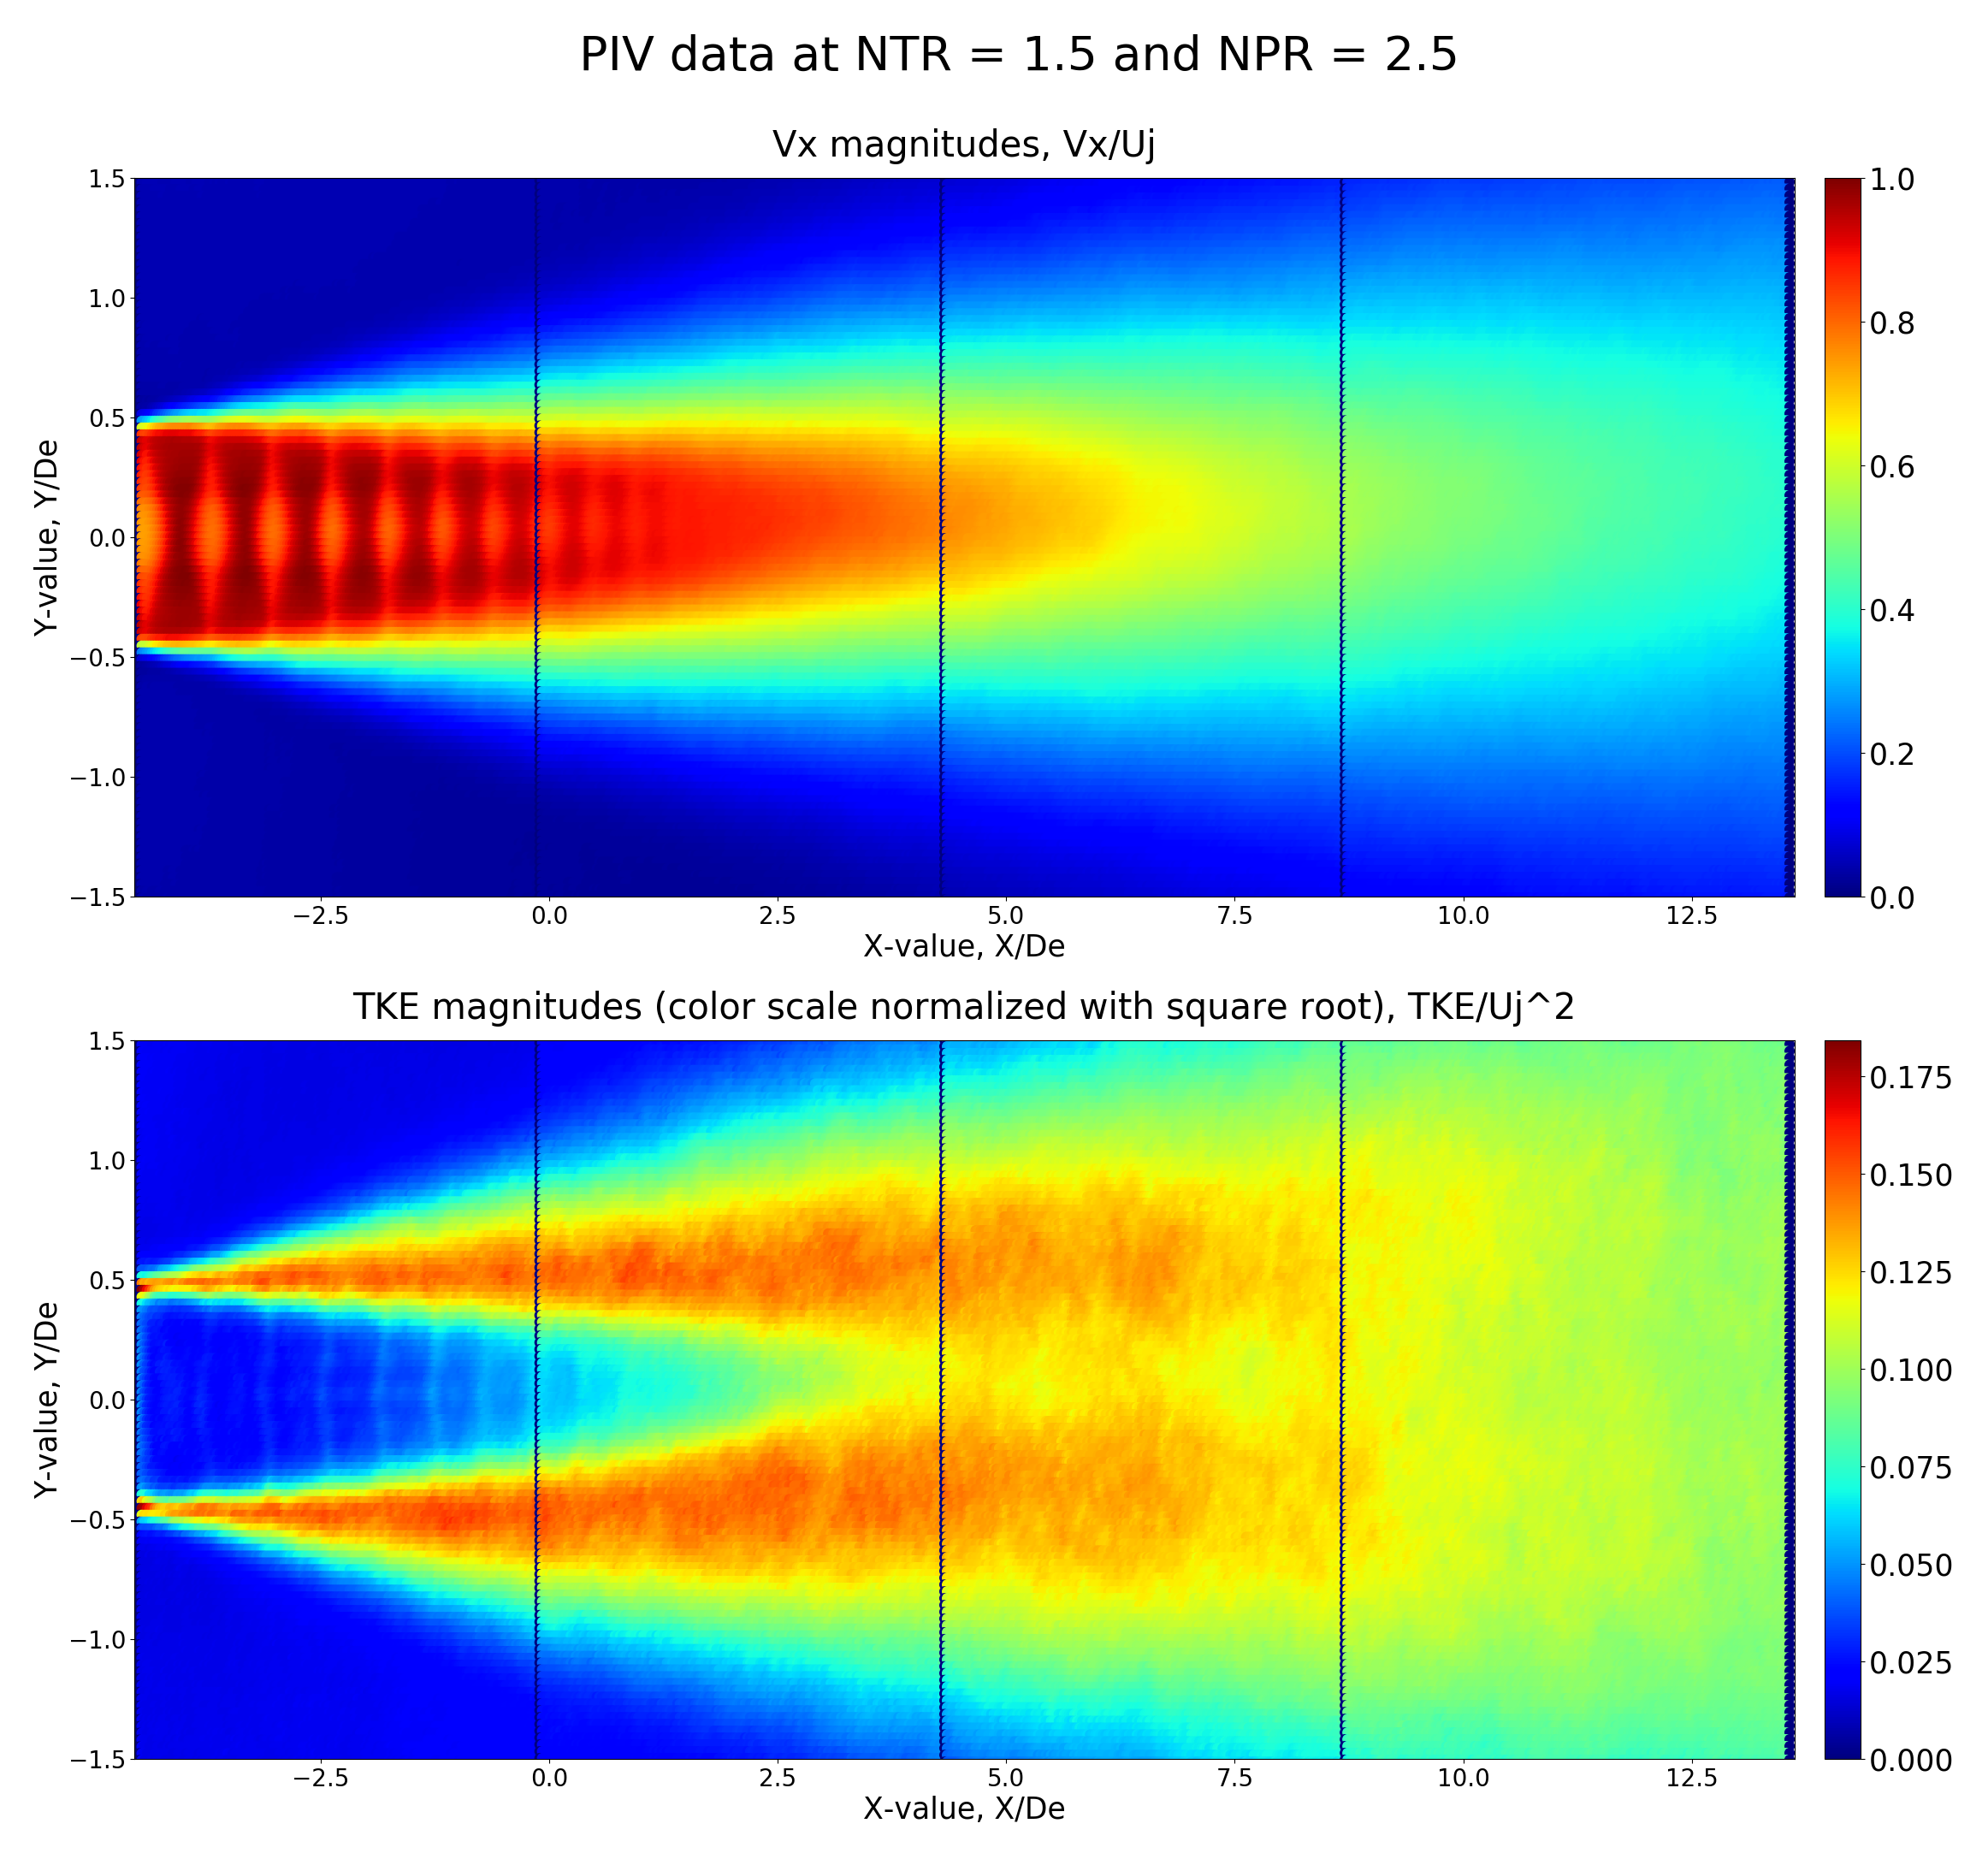
\includegraphics[width=2.3in]{images/PIV_NTR1p5_NPR2p5.png}
	\caption{NTR:1p5 NPR:2p5 }
	\label{fig:setup1}
\end{subfigure}%
\begin{subfigure}{.5\textwidth}
	\centering
	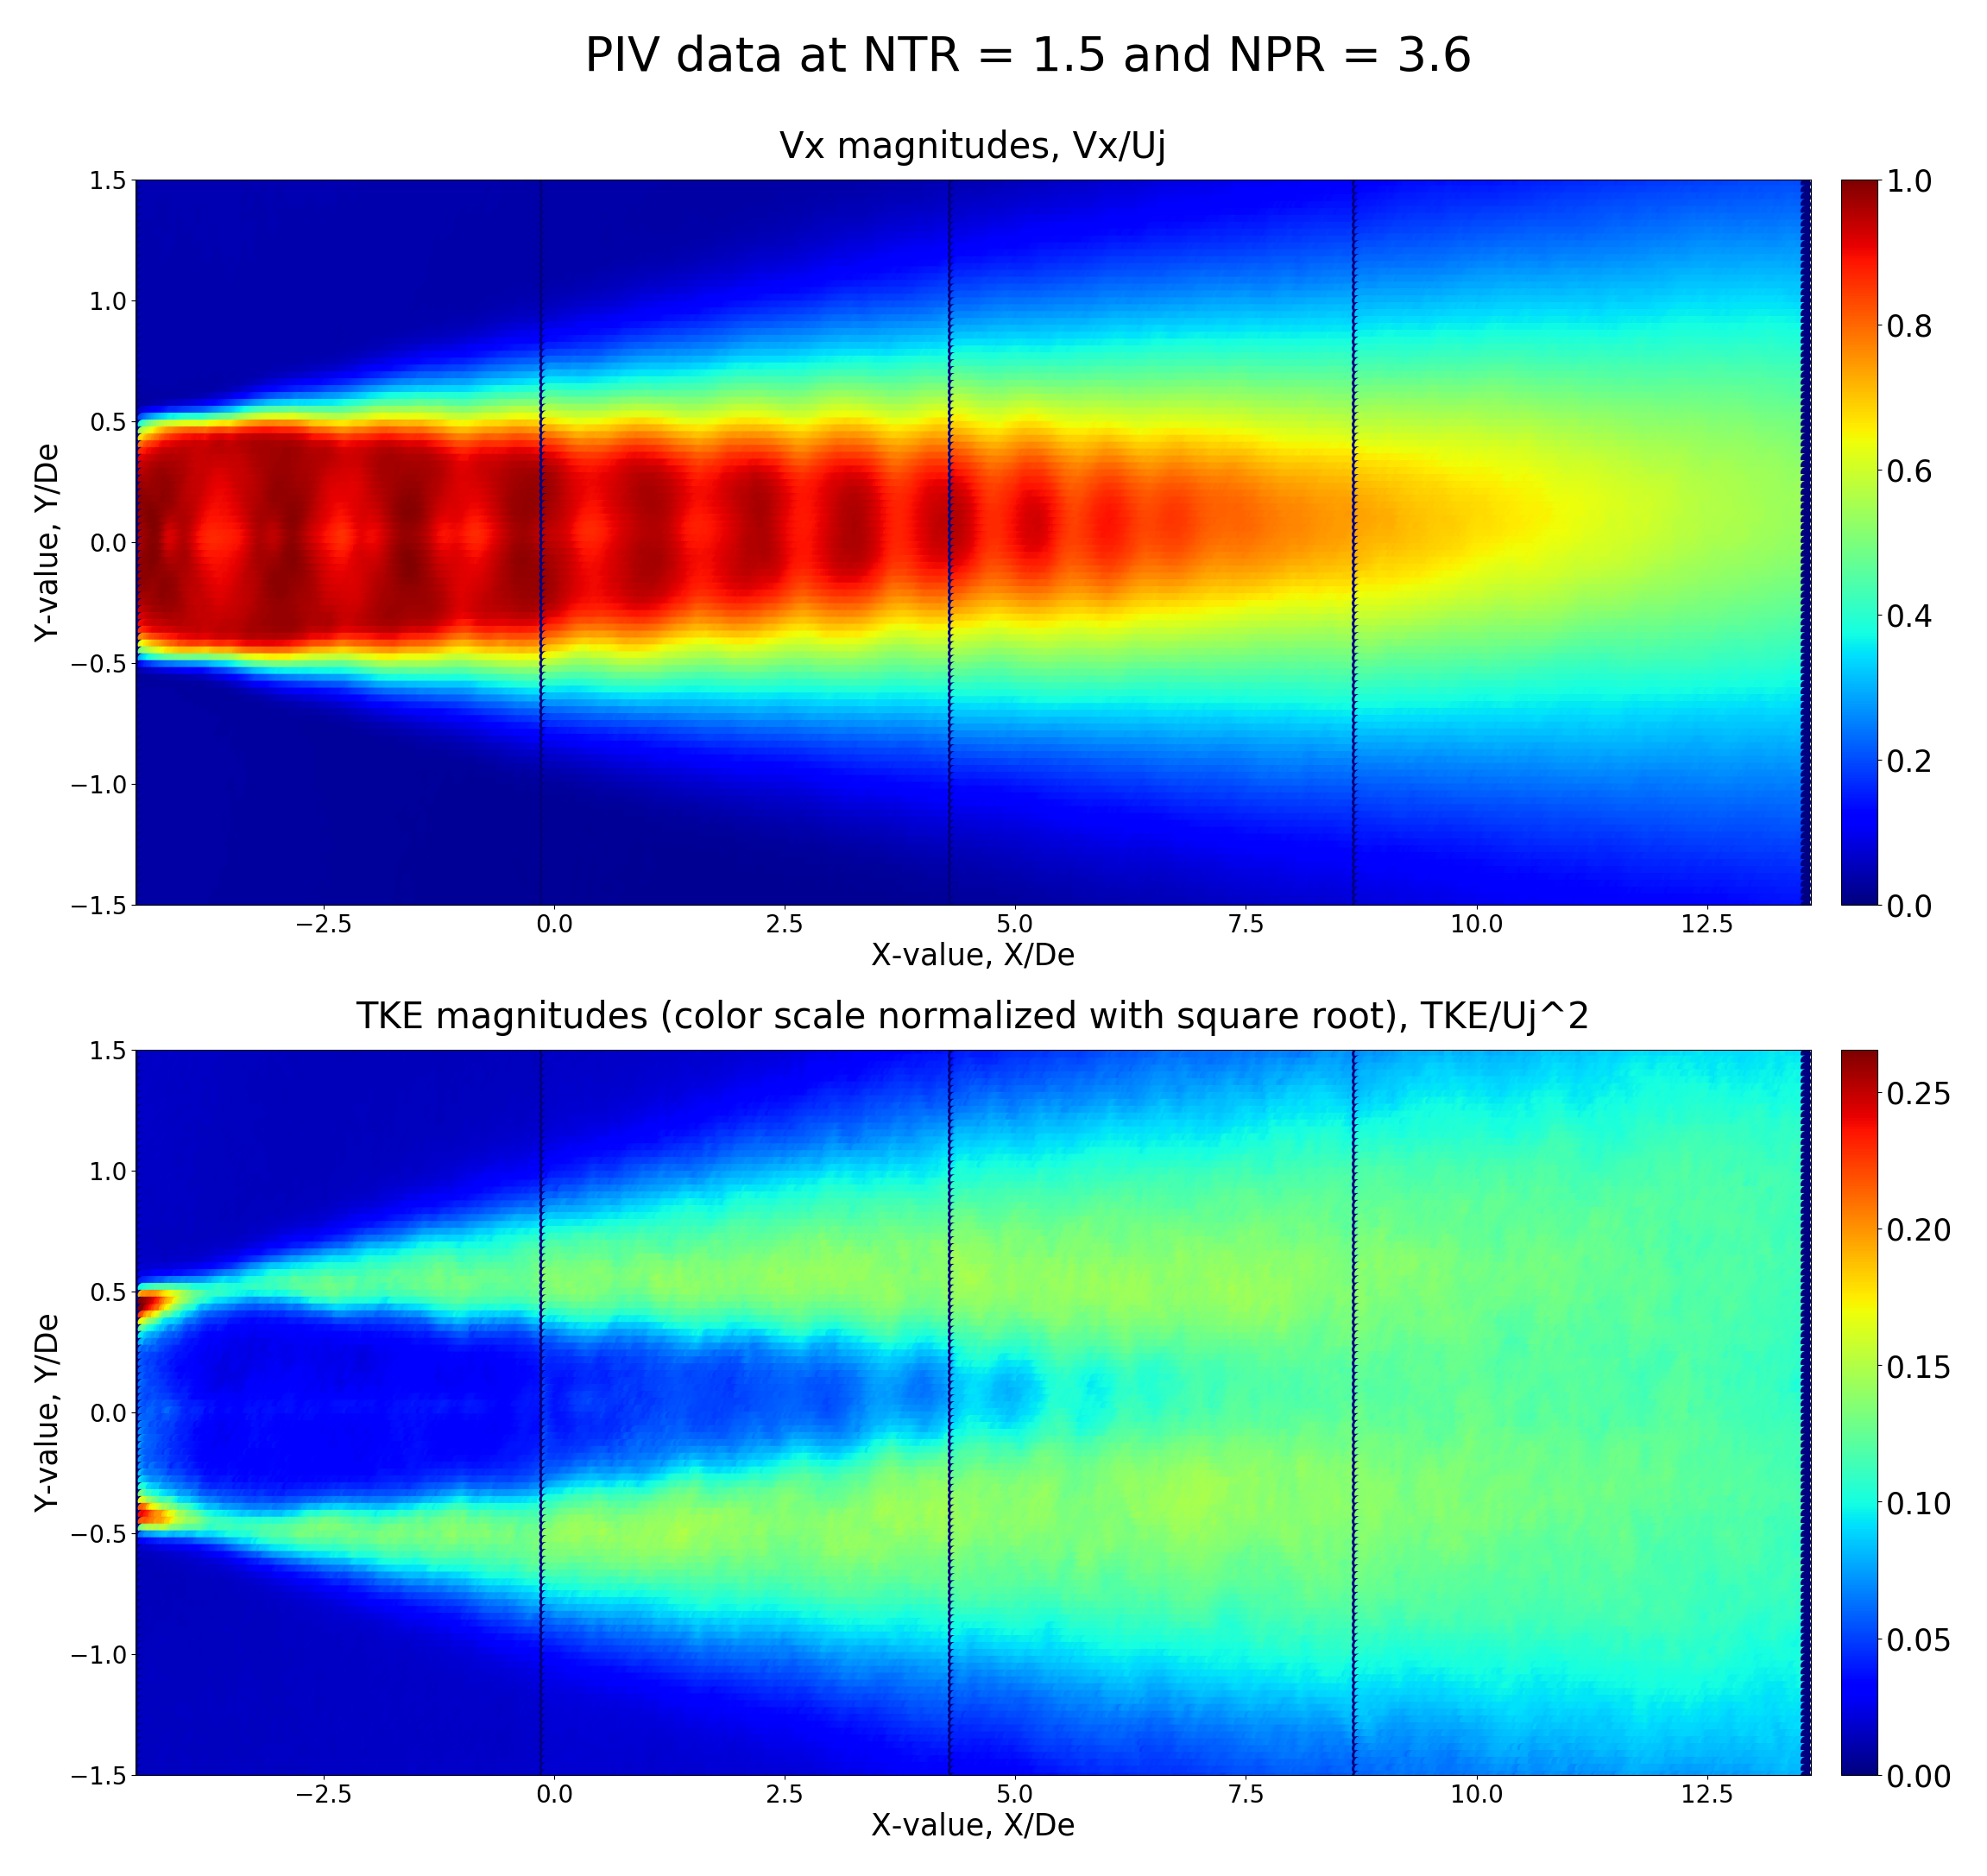
\includegraphics[width=2.3in]{images/PIV_NTR1p5_NPR3p6.png}
	\caption{NTR:1p5 NPR:3p6 }
	\label{fig:setup2}
\end{subfigure}
\begin{subfigure}{1.0\textwidth}
	\centering
	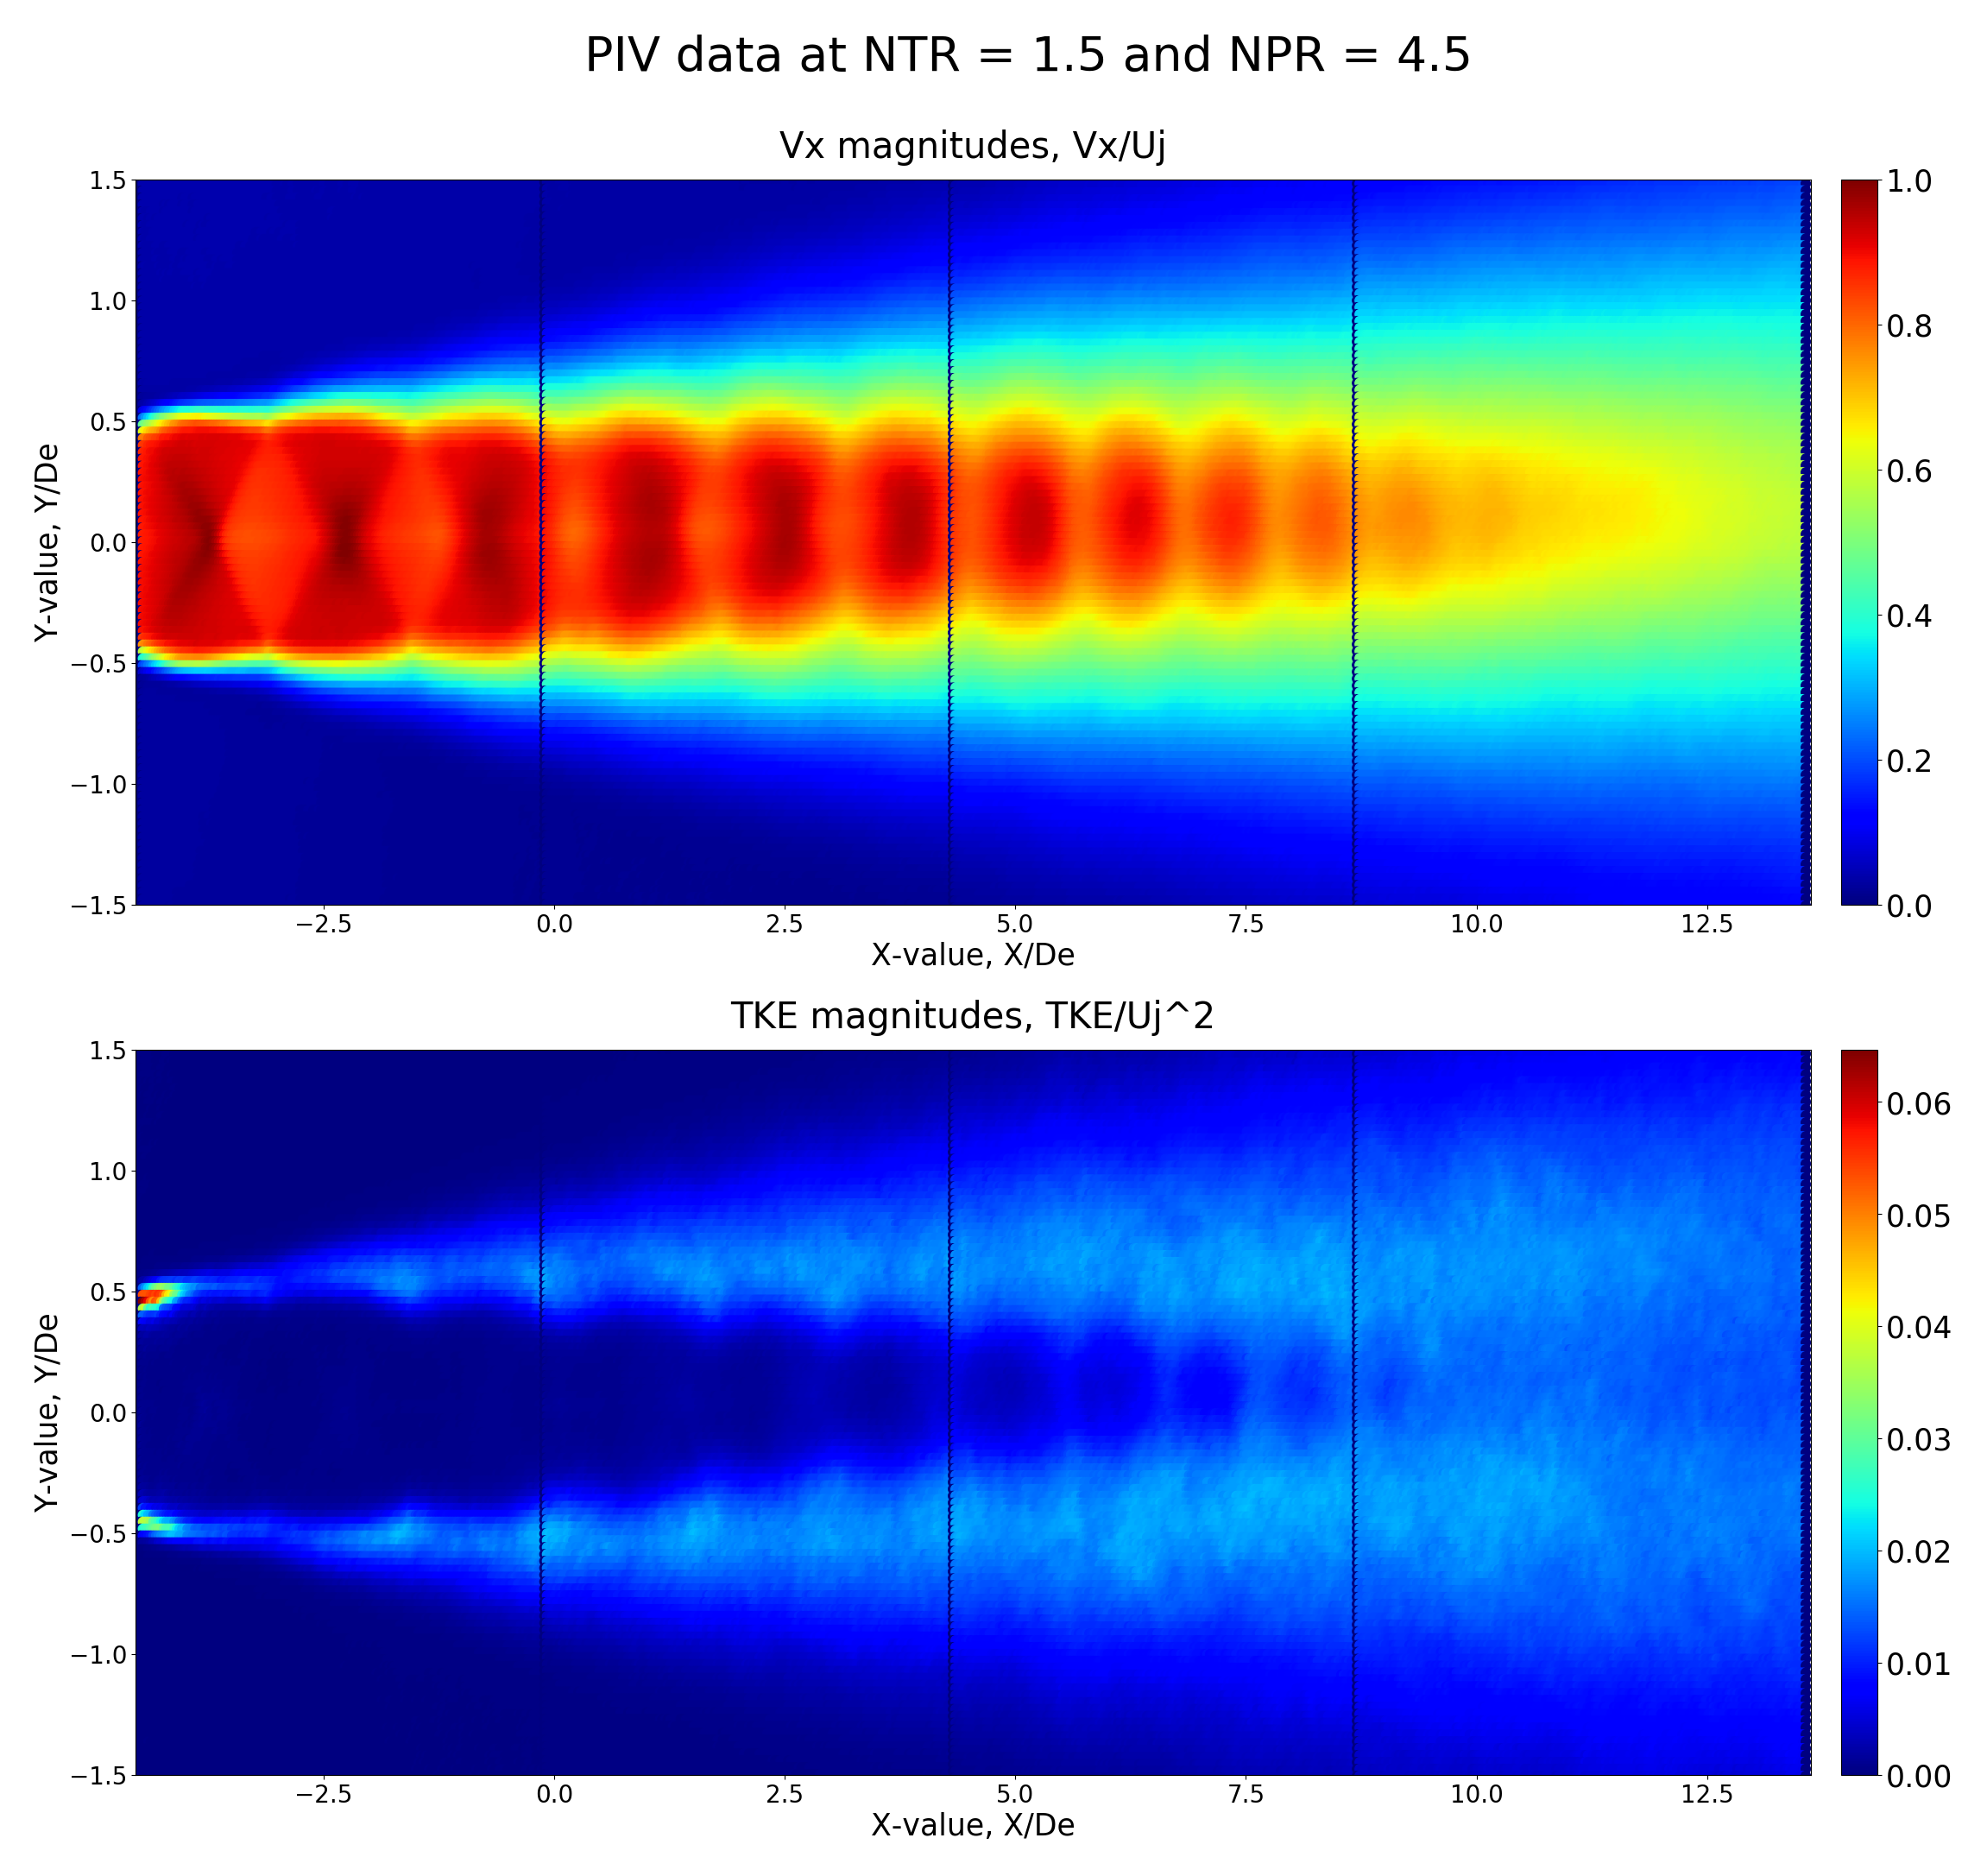
\includegraphics[width=2.3in]{images/PIV_NTR1p5_NPR4p5.png}
	\caption{NTR:1p5 NPR:4p5 }
	\label{fig:setup2}
\end{subfigure}
\caption{$V_x$, TKE without chevrons at $M_d$ 1.5 }
\label{fig:2dplots}
\end{figure}

\section{Shock cell length}
For an ideally expanded flow; assuming $D_j$, $M_j$ same as $D_e$,$M_d$; shock cell length can be calculated from equation \ref{eq:1}  to be 1.46$D_e$. It is expected to be higher for underexpanded flow and lower for overexpanded flow because of the differences in $D_j$ and $D_e$. Since $M_j$ decreases along the flow, this shock length is usually among the highest of all the wavelengths seen in the spectrum.\\ 

\begin{figure}[H]
\begin{subfigure}{.5\textwidth}
	\centering
	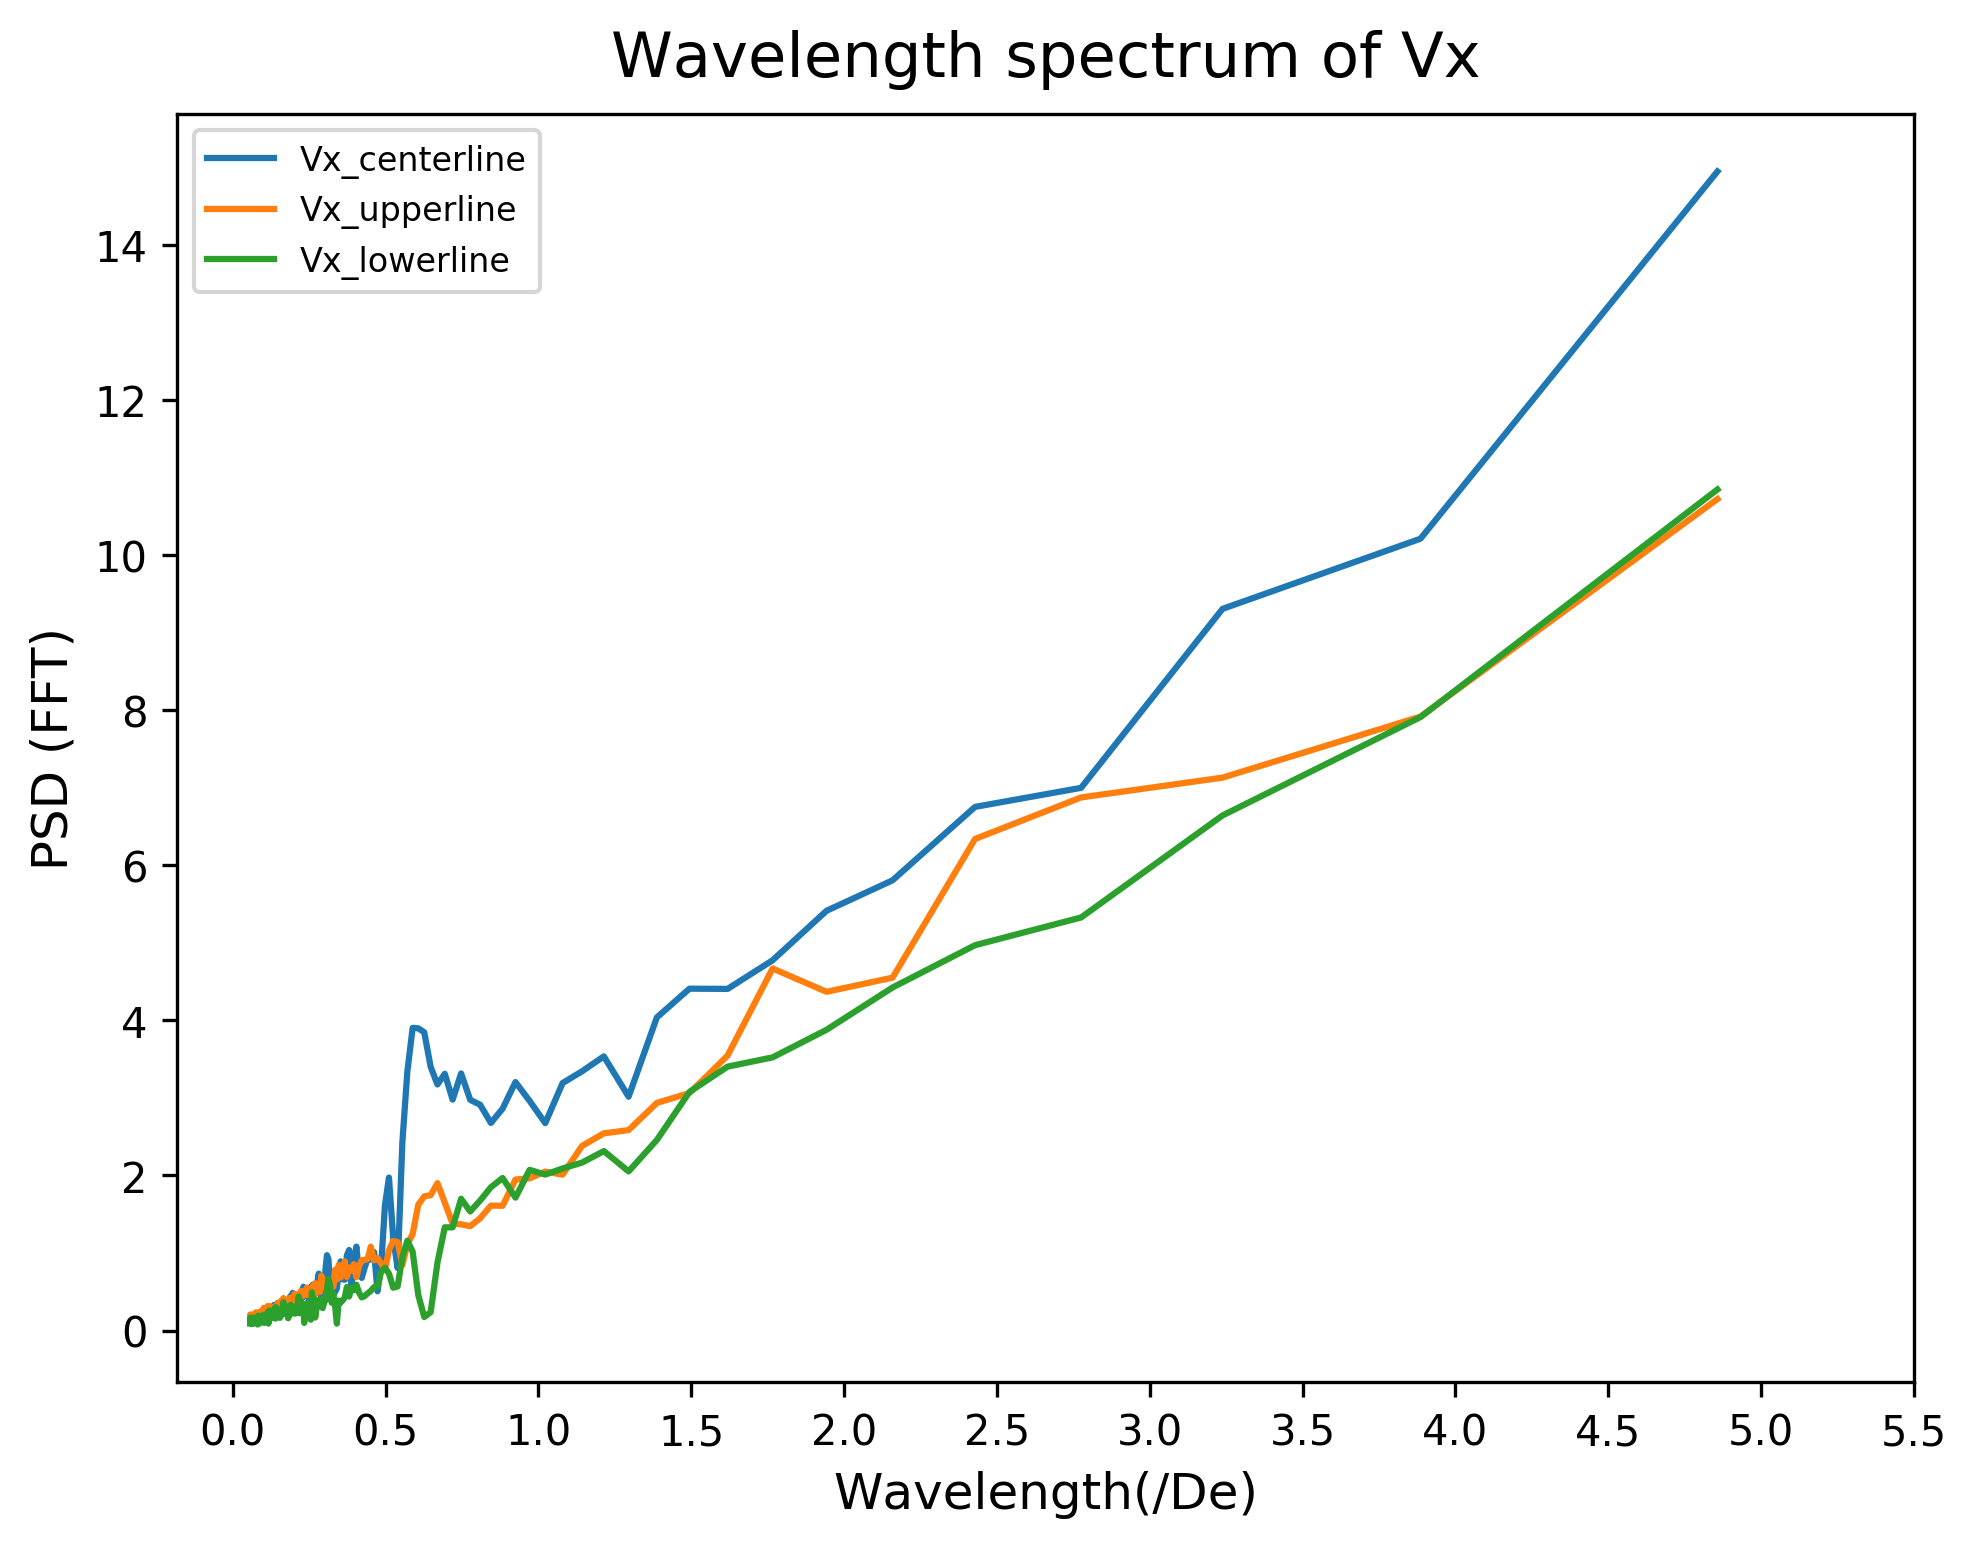
\includegraphics[width=2.5in]{images/Fft_Vx_NTR1p5_NPR2p5.png}
	\caption{NTR:1p5 NPR:2p5 }
	\label{fig:setup1}
\end{subfigure}%
\begin{subfigure}{.5\textwidth}
	\centering
	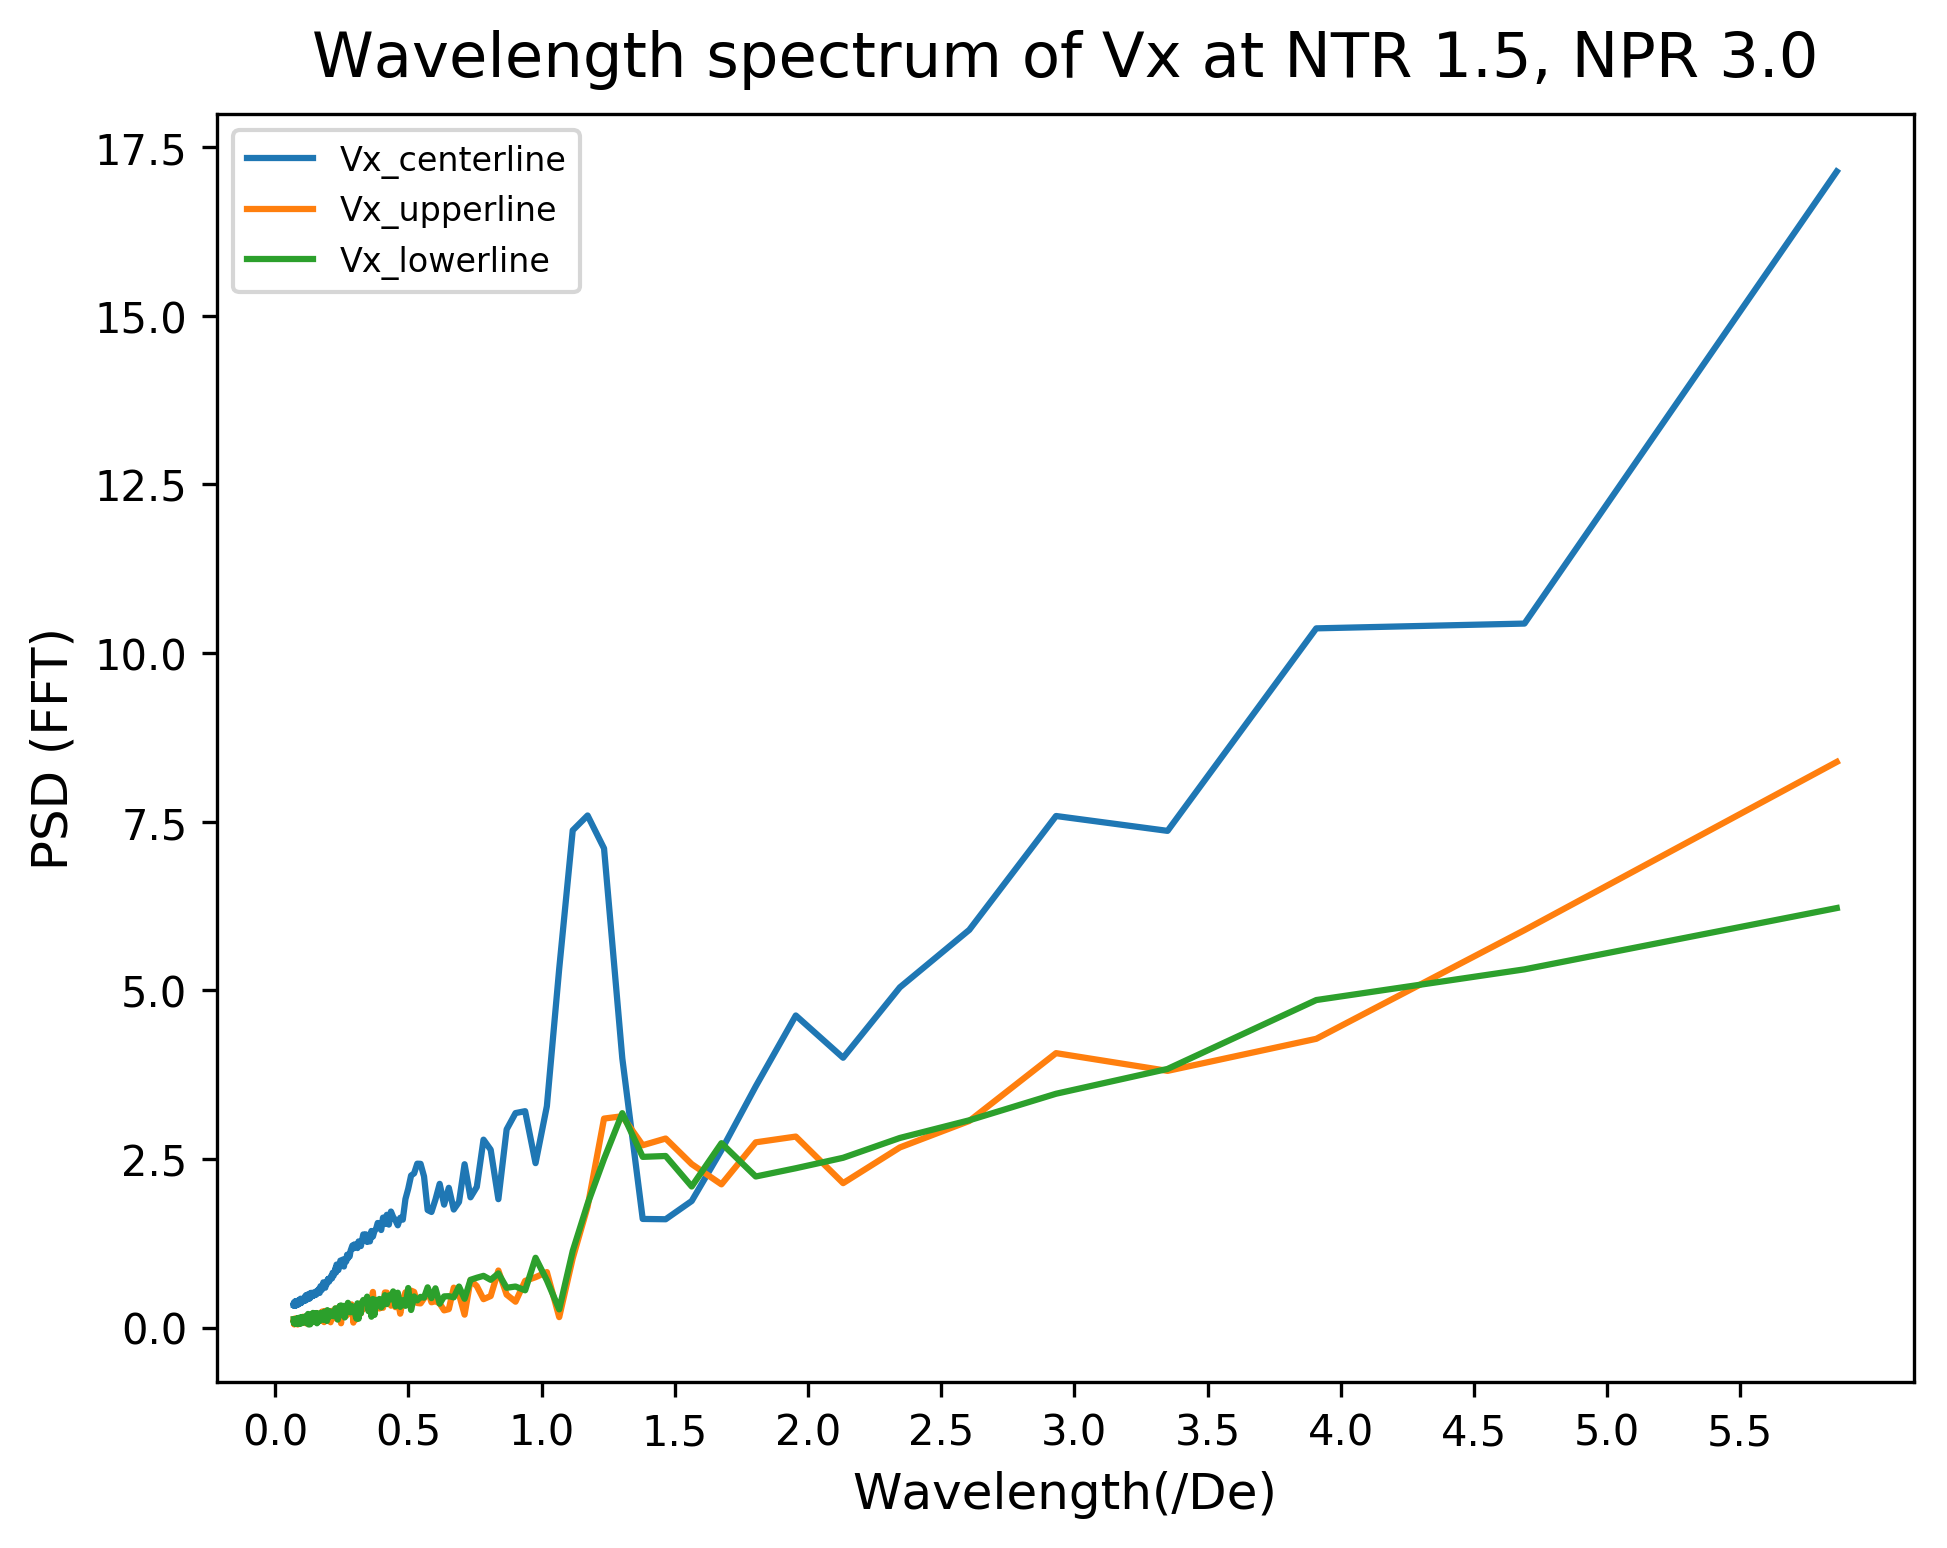
\includegraphics[width=2.5in]{images/Fft_Vx_NTR1p5_NPR3p0.png}
	\caption{NTR:1p5 NPR:3p0 }
	\label{fig:setup2}
\end{subfigure}
\begin{subfigure}{0.5\textwidth}
	\centering
	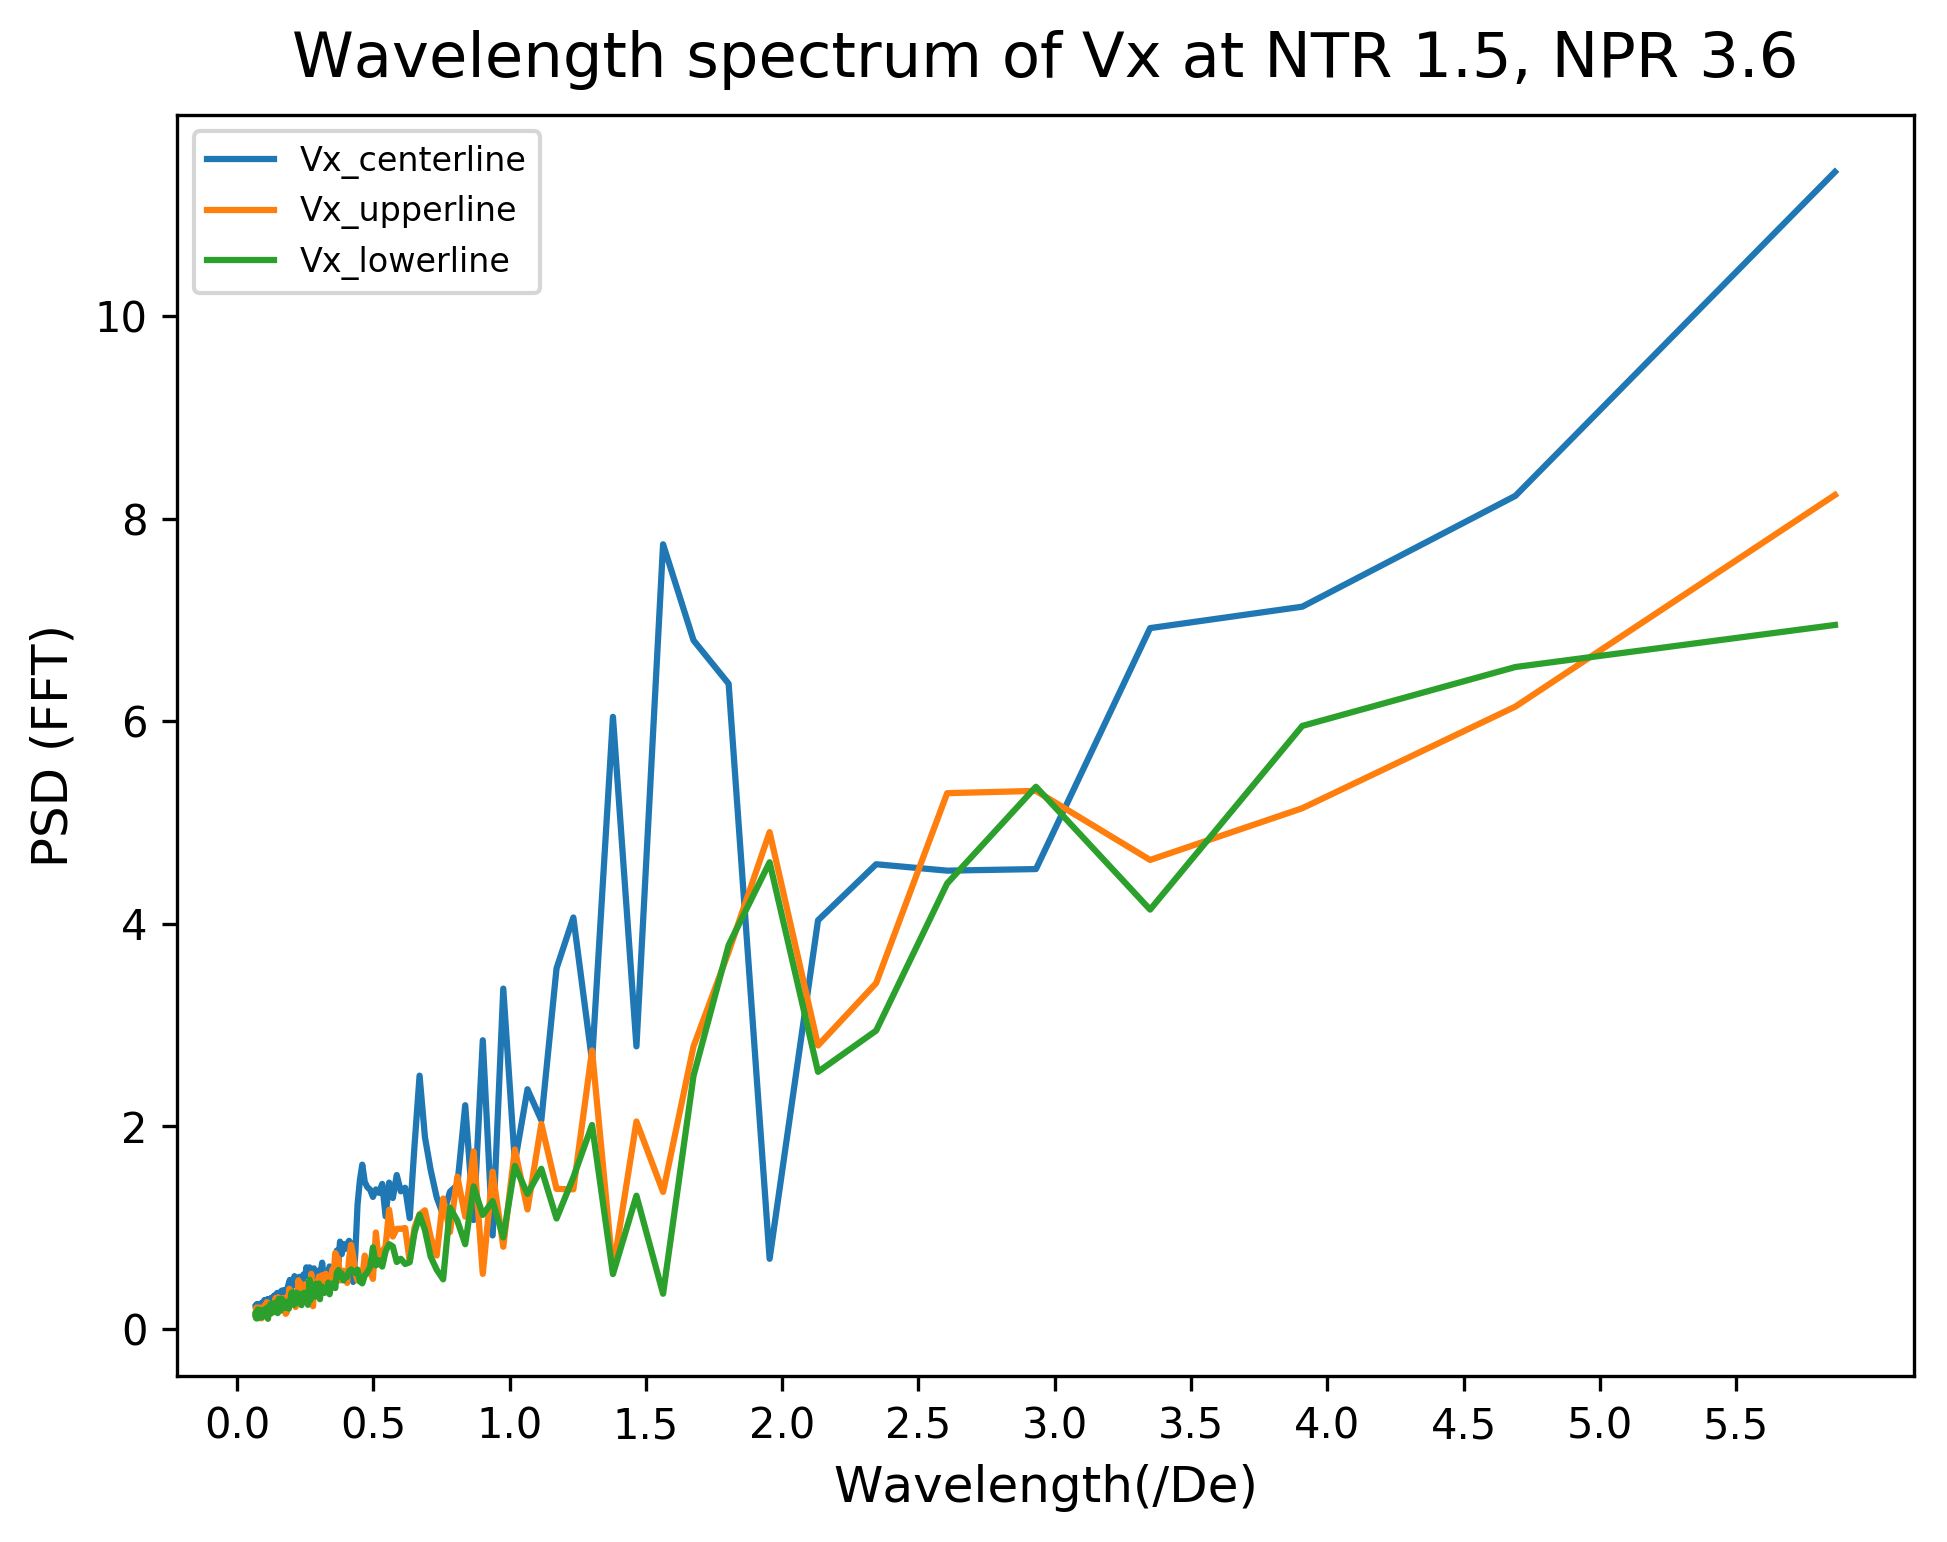
\includegraphics[width=2.5in]{images/Fft_Vx_NTR1p5_NPR3p6.png}
	\caption{NTR:1p5 NPR:3p6 }
	\label{fig:setup2}
\end{subfigure}
\begin{subfigure}{0.5\textwidth}
	\centering
	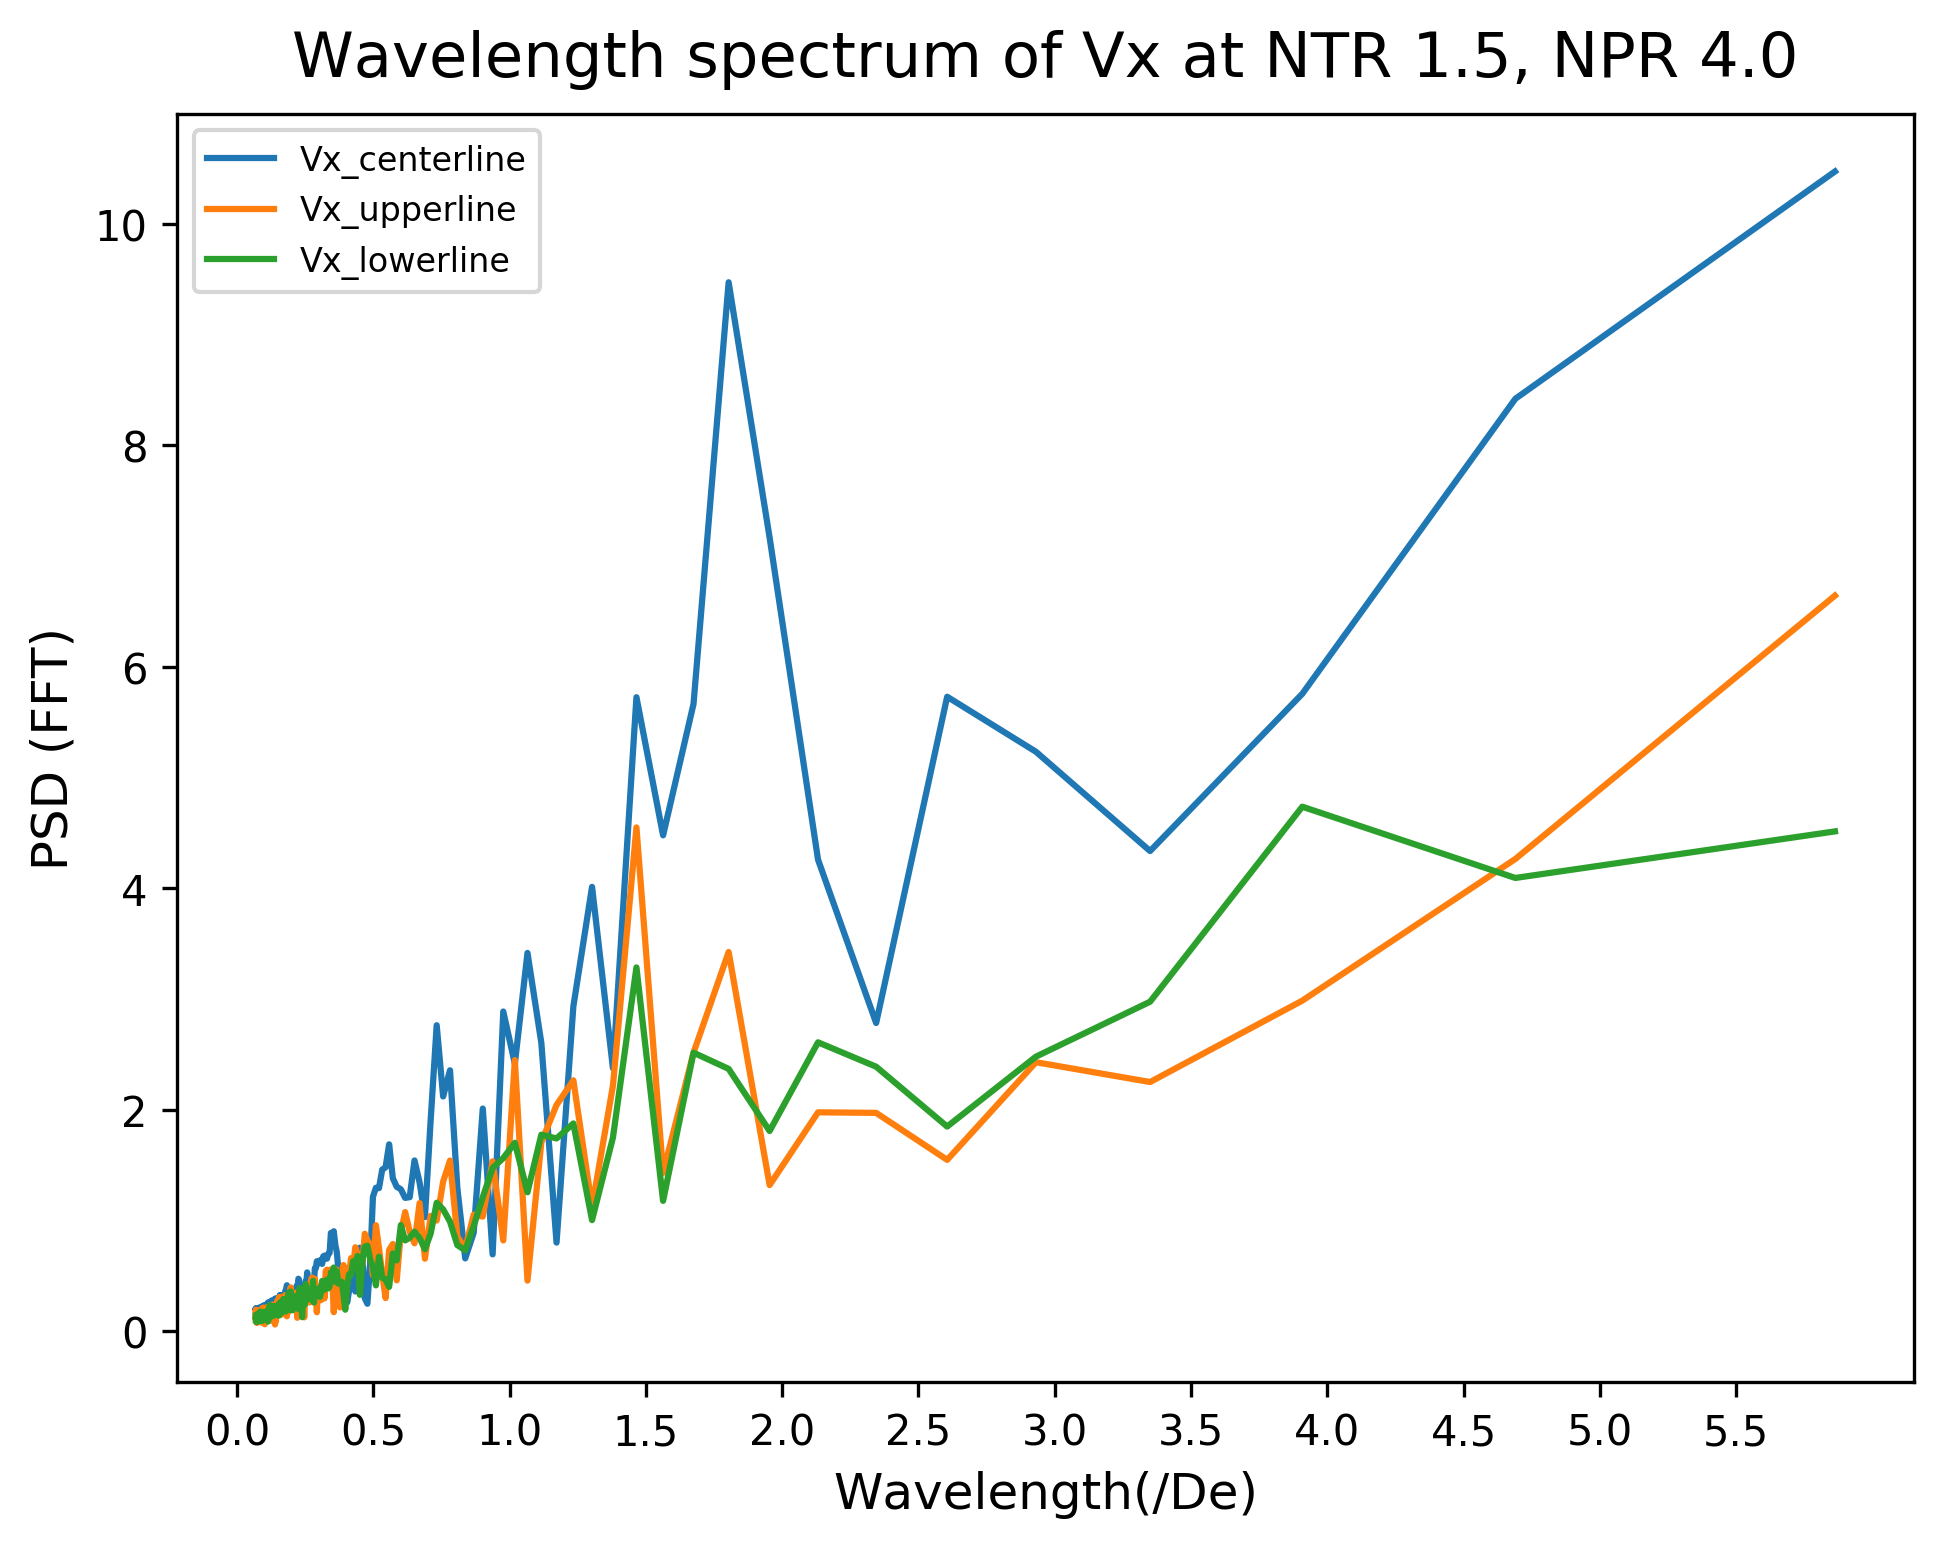
\includegraphics[width=2.5in]{images/Fft_Vx_NTR1p5_NPR4p0.png}
	\caption{NTR:1p5 NPR:4p0 }
	\label{fig:setup2}
\end{subfigure}
\begin{subfigure}{1.0\textwidth}
	\centering
	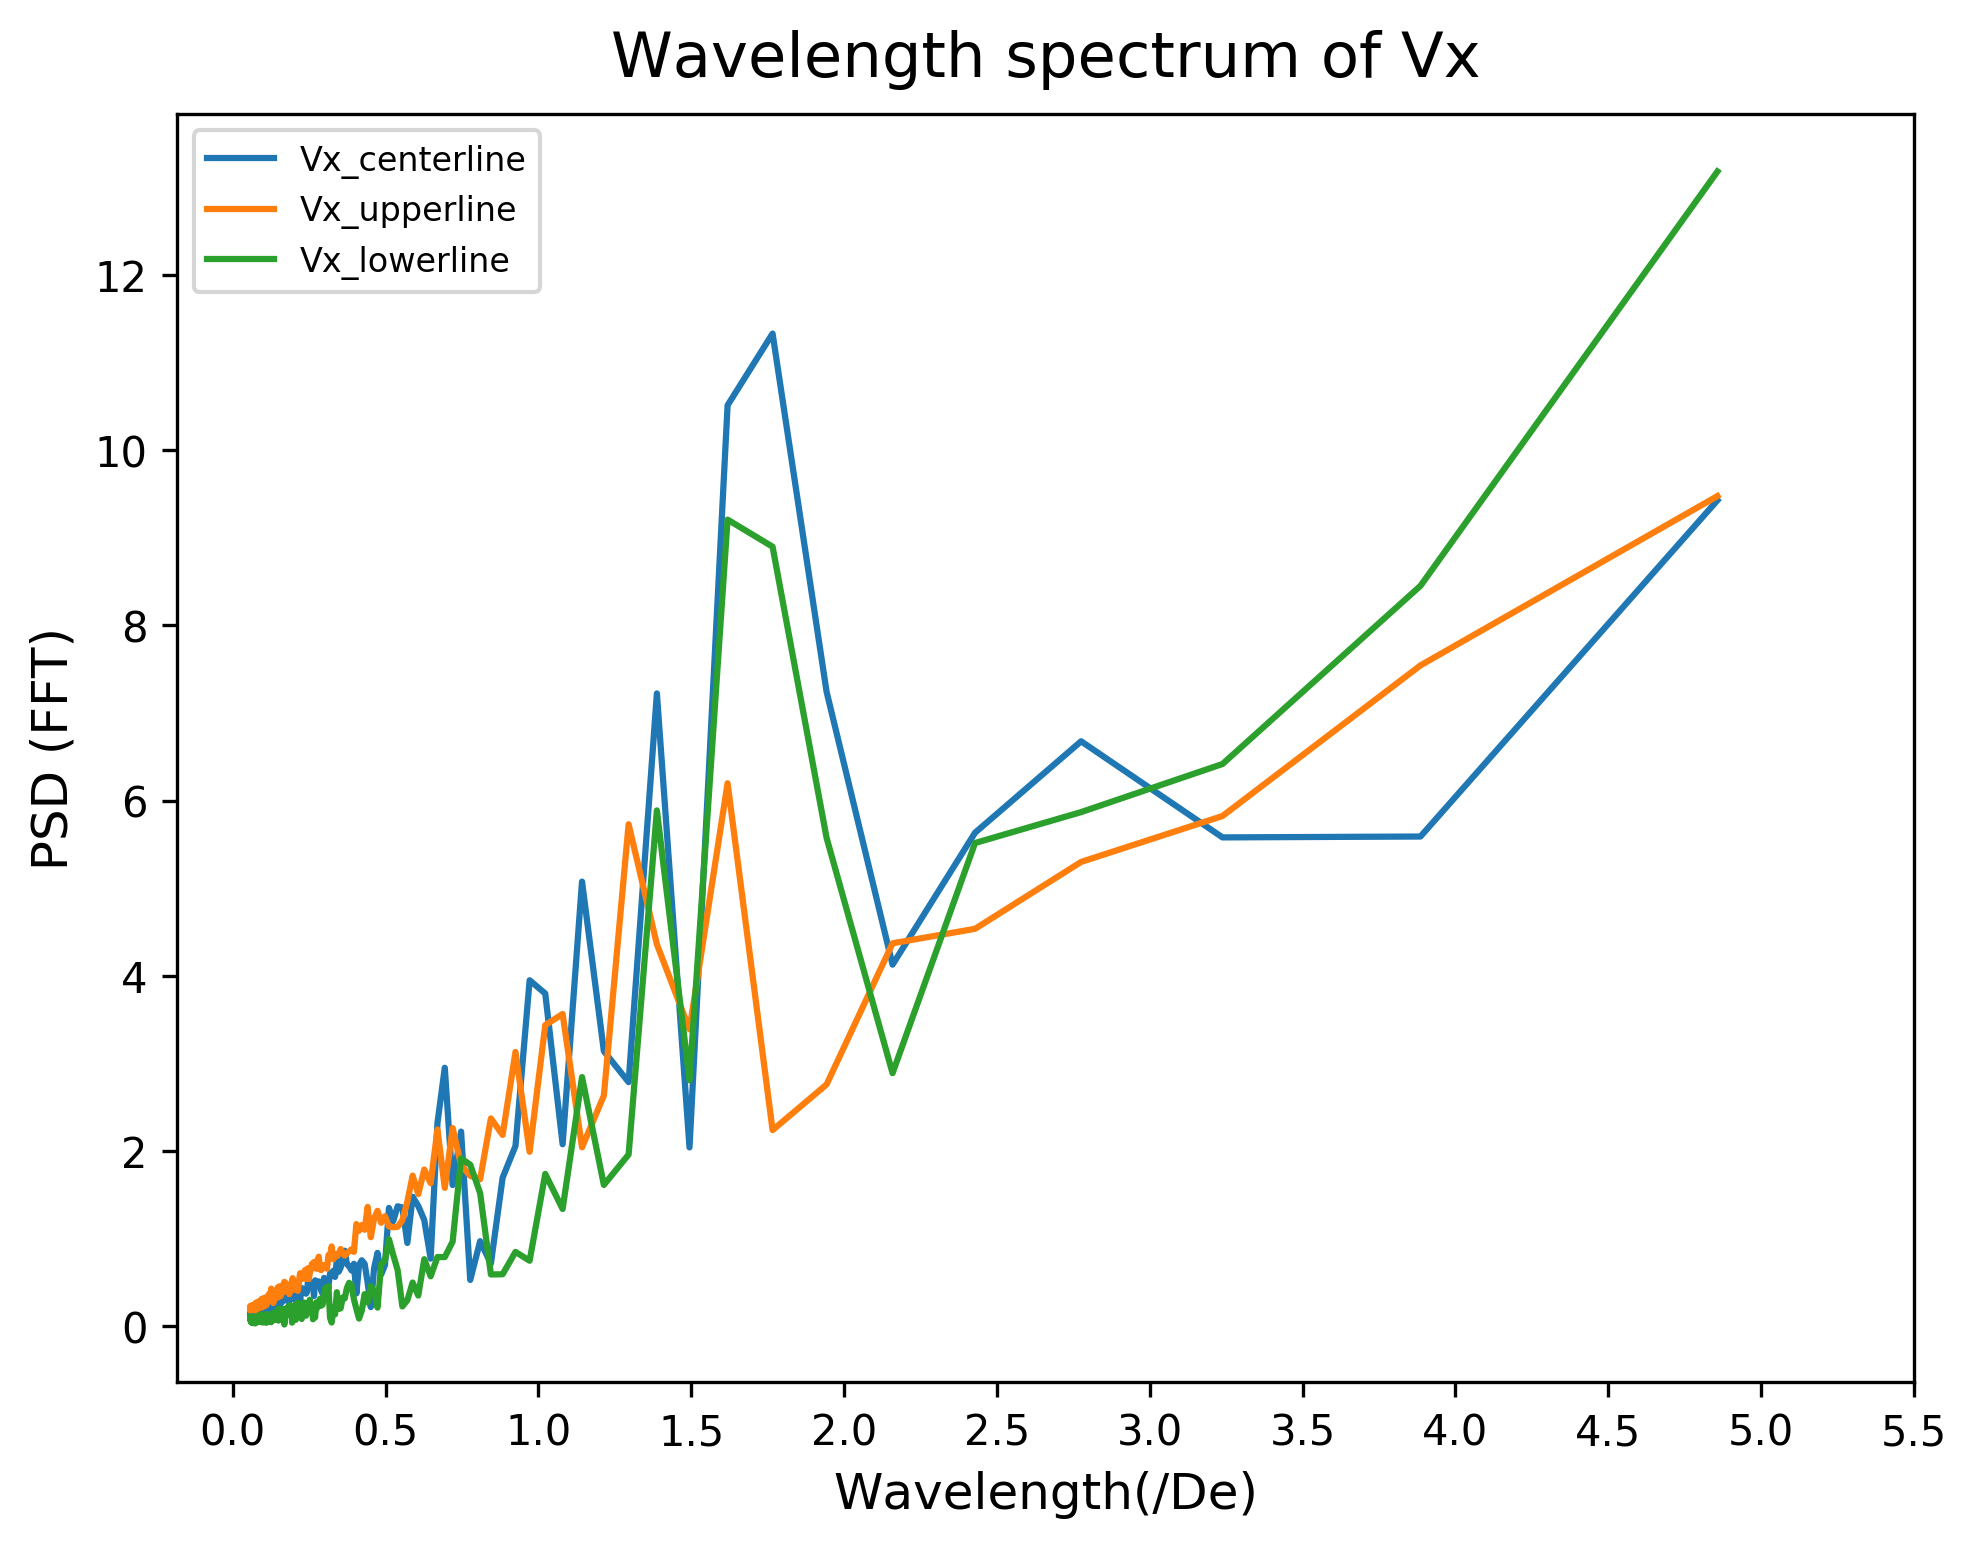
\includegraphics[width=2.5in]{images/Fft_Vx_NTR1p5_NPR4p5.png}
	\caption{NTR:1p5 NPR:4p5 }
	\label{fig:setup2}
\end{subfigure}
\caption{Wavelength spectrum using FFT for $V_x$ centreline data without chevrons}
\label{fig:fftplots}
\end{figure}

As we see in the FFT plots (fig \ref{fig:fftplots}), for ideally expanded flow, shock cell wavelength is close to the value earlier calculated. As the pressure increases, wavelength with maximum psd increases. We can notice that in 2d plots too(fig \ref{fig:2dplots}). It is also interesting to note that the wavelengths are well defined for underexpanded flows because of the few oblique shocks. For overexpanded flows, since the shocks are due to the large number of reflected expansion waves, the wavelength pattern is more rugged. So is the case for near perfectly expanded flow.\\

Inlet temperature doesn't seem to have major effect on wavelength pattern. Although when the NTR is 3.0, wavelength is clearly subdued. This shows that the shocks are not as intense as of colder flows \\

\section{Merging of shocks and shear layers}
If we carefully observe in the fig \ref{fig:2dplots}, two shocks exist at the lip forming double delta pattern which merge later in the jet wake. Although NPR was close to perfect expansion which should give only shocks reflected inside the nozzle, imperfections in equipment might be the reason for multiple shock structures. TKE at the lips seems to be highest, which shows the importance of screech tone generation. It is easier to notice the shocks merging in lineplots of $V_x$ (fig \ref{fig:lineplotsVx}) when compared to 2D plots. Shocks originated before jet exit seem to run slower than the ones generated after, finally merging with the shear layer shocks.\\ 
 
\begin{figure}[H]
\begin{subfigure}{.5\textwidth}
	\centering
	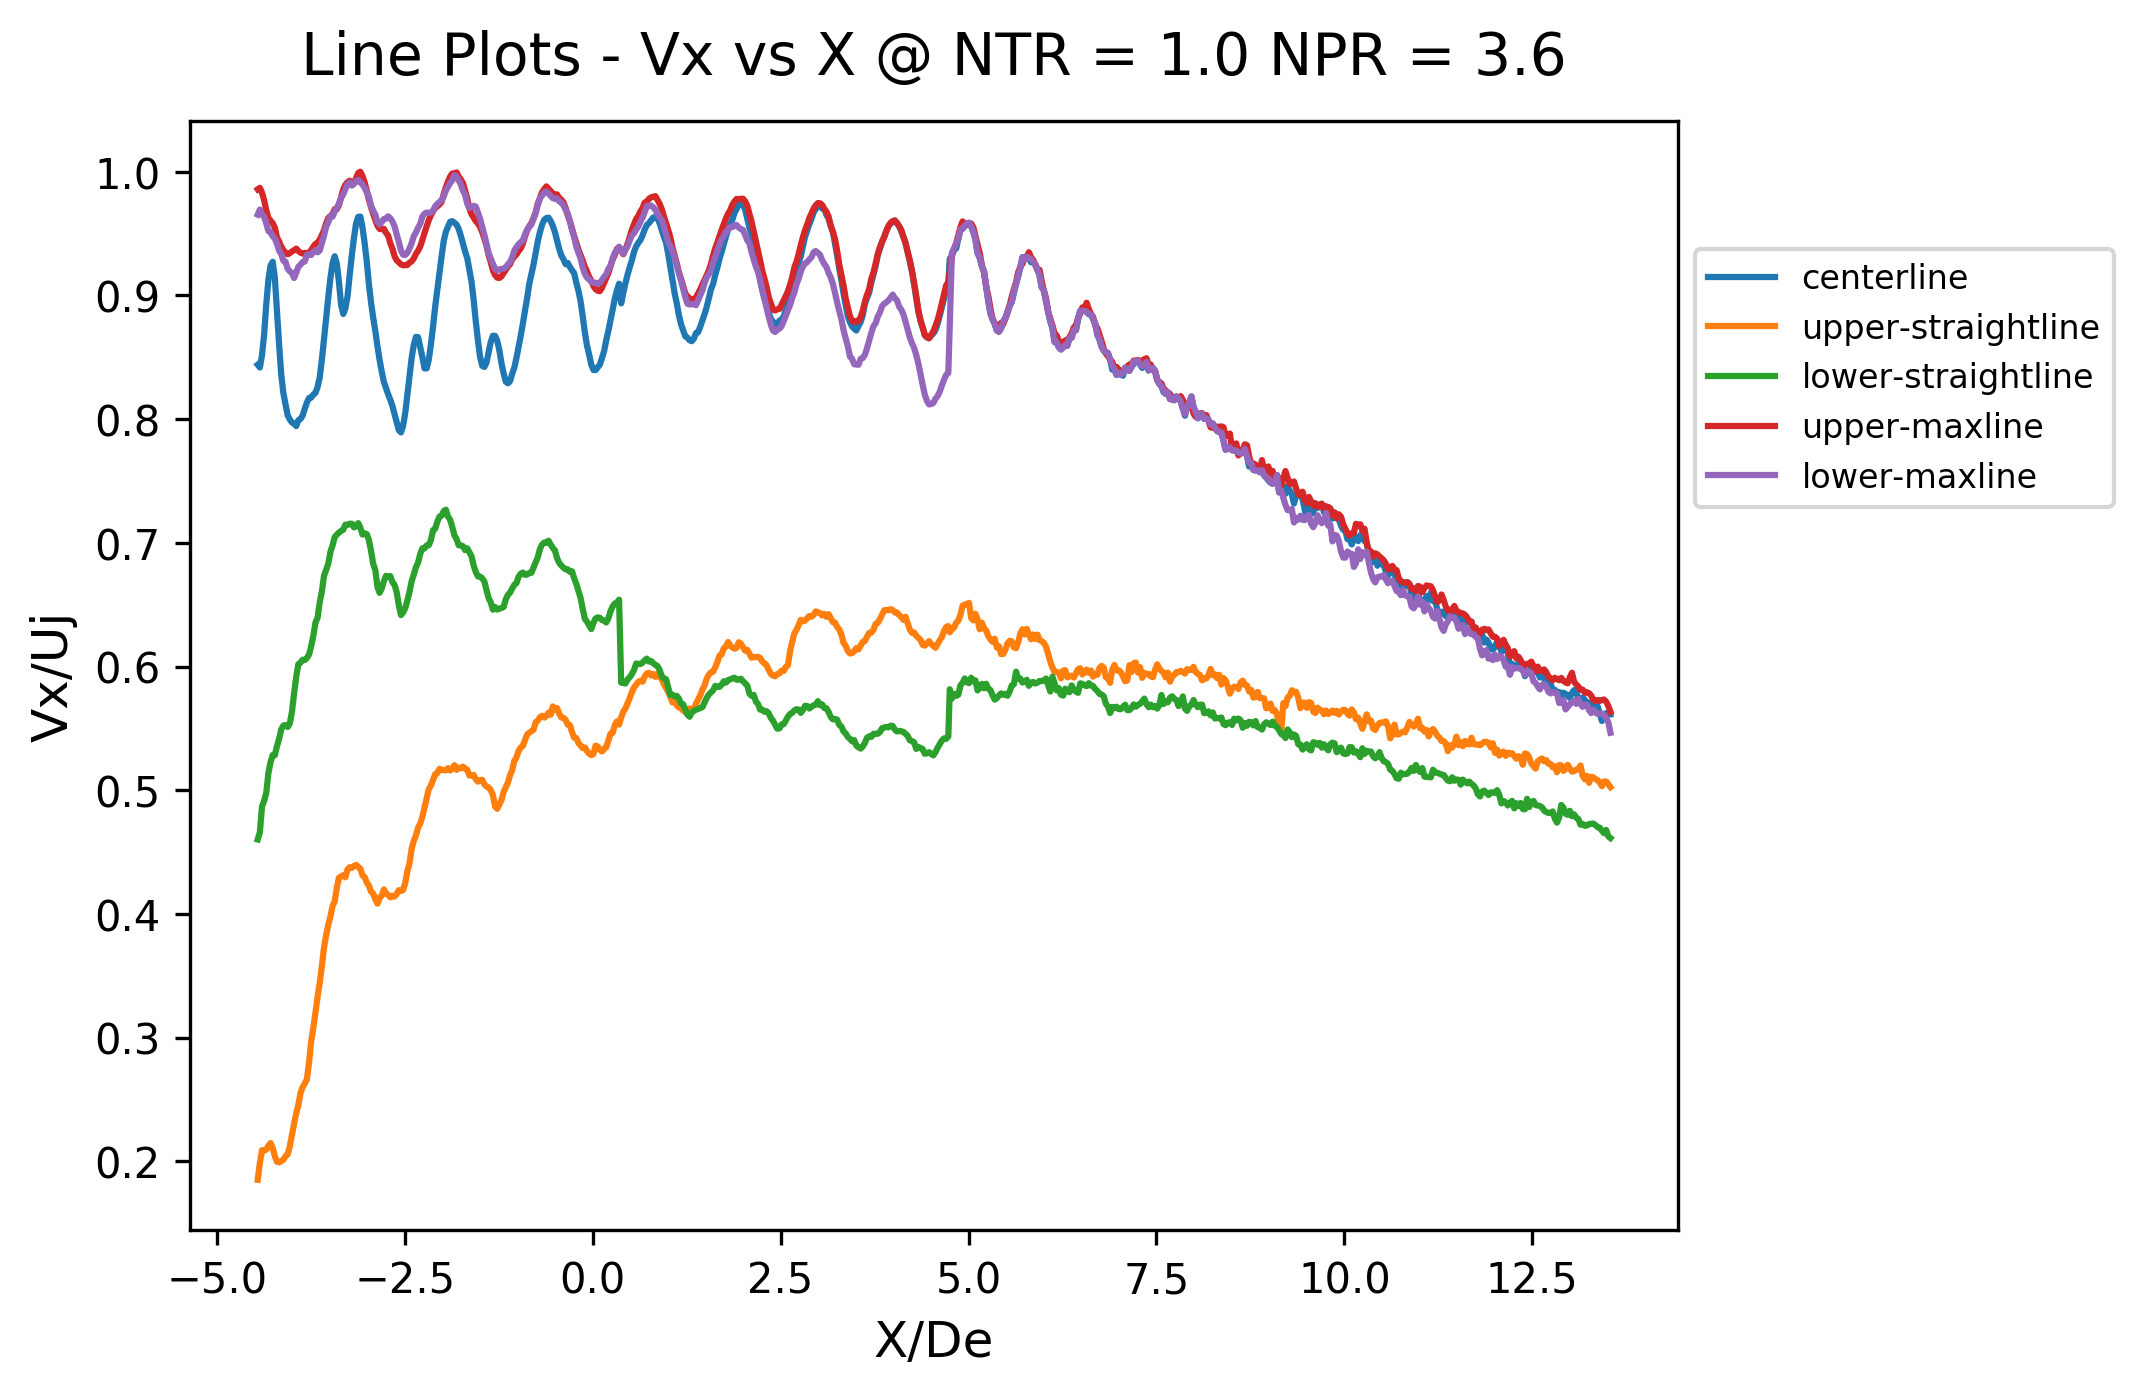
\includegraphics[width=3in]{images/LinePlots_Vx_NTR1p0_NPR3p6.png}
	\caption{NTR:1p0 NPR:3p6 }
	\label{fig:setup1}
\end{subfigure}%
\begin{subfigure}{.5\textwidth}
	\centering
	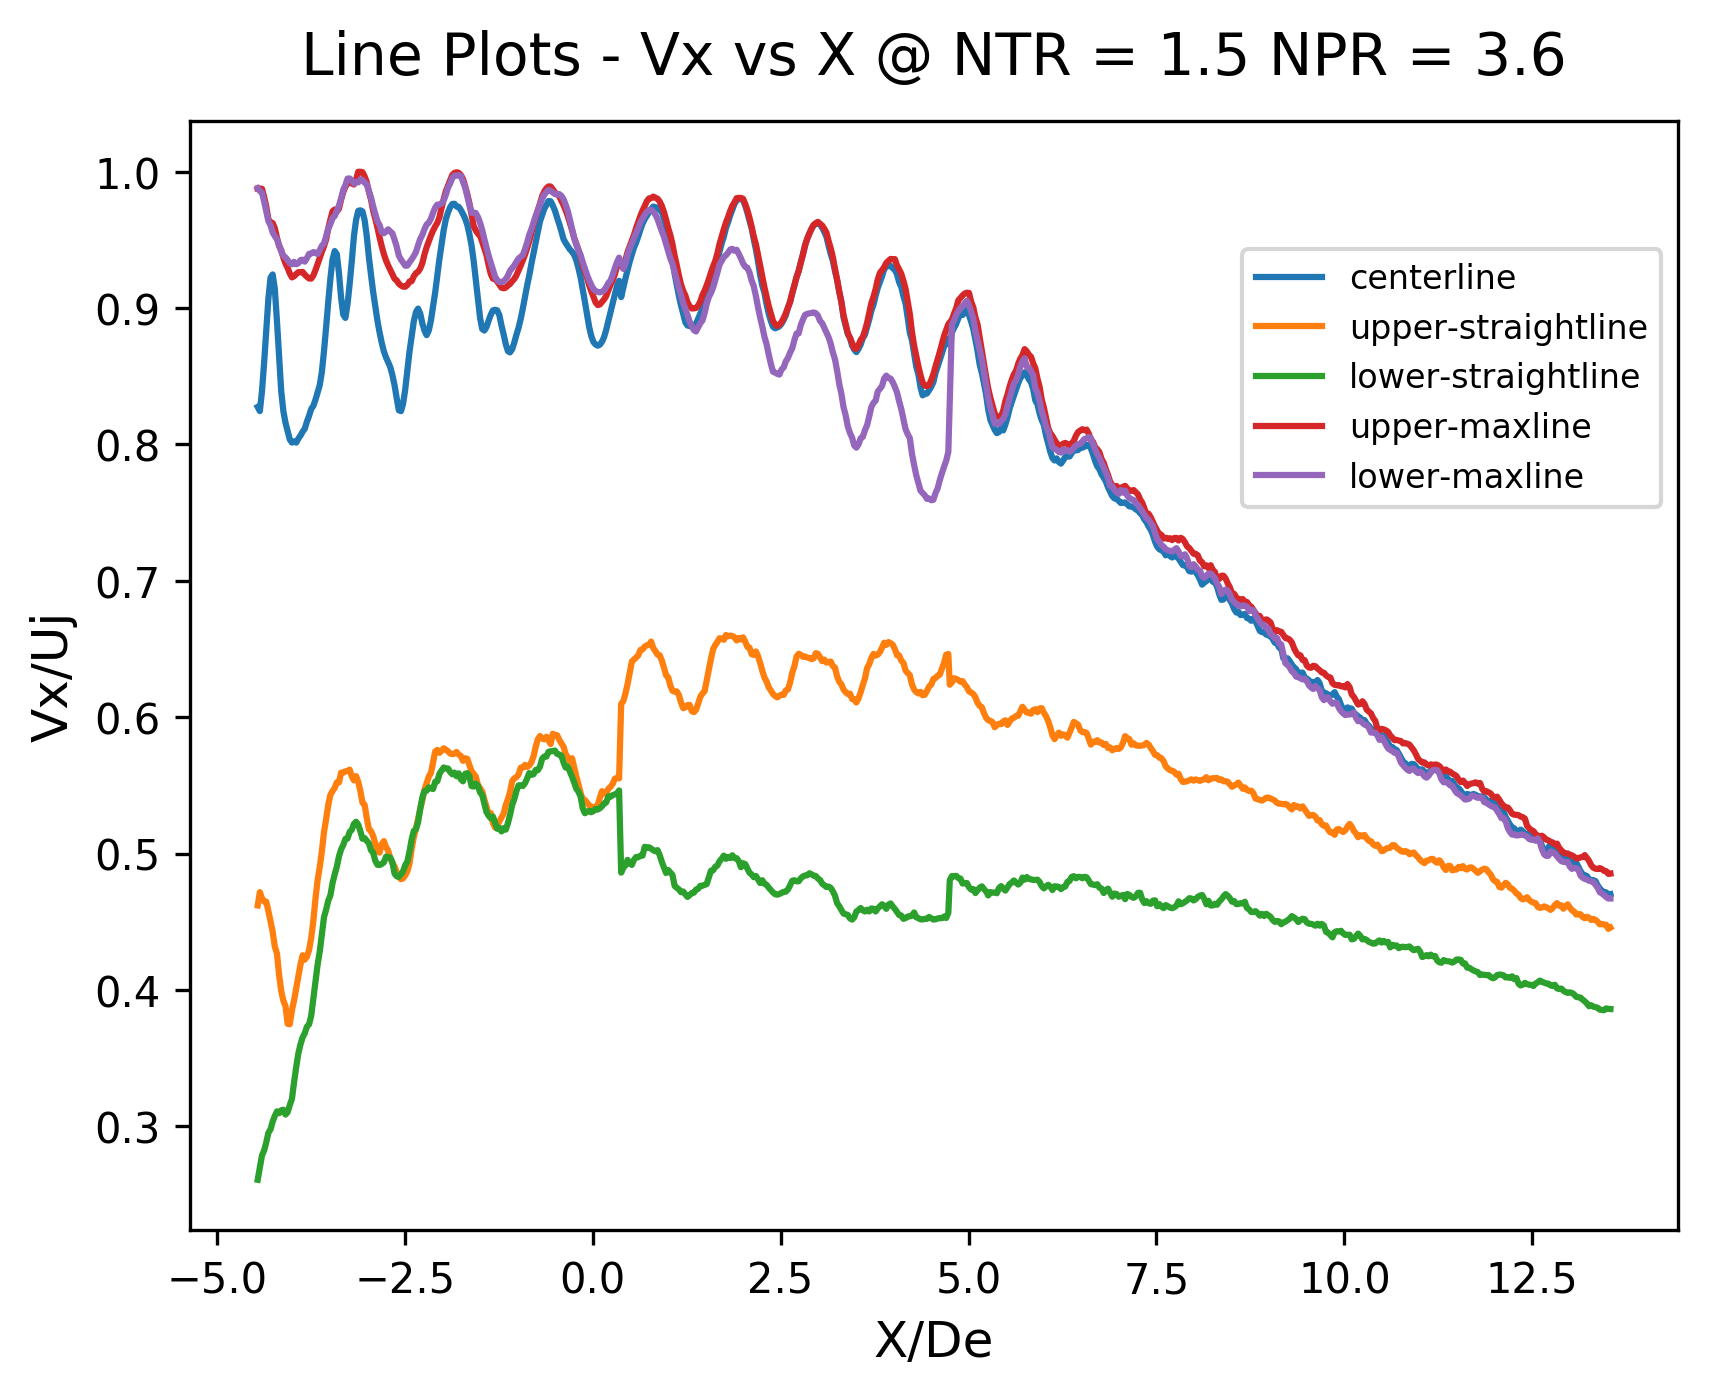
\includegraphics[width=2.5in]{images/LinePlots_Vx_NTR1p5_NPR3p6.png}
	\caption{NTR:1p5 NPR:3p6 }
	\label{fig:setup2}
\end{subfigure}
\caption{centreline plots for $V_x$ without chevrons }
\label{fig:lineplotsVx}
\end{figure} 

Spectograms are another way to interpret lineplots data. From fig \ref{fig:spectogramVx}, most of the spectrum seem to be around the wavenumber (1/wavelength) that we calculated analytically and also noticed in FFT plots(fig \ref{fig:fftplots}). Precision is not high as the sampling data is small, but it gives an idea of spectrum at every point along jet. Multiple wavenumbers merging to form a single broad smudge shows merging of shocks and decrease substantially showing the end of potential core because of merging of shear layers. Spectogram of TKE(fig \ref{fig:spectogramTKE}) can also be similarly used to estimate the end of potential core. This wavelength spectrum could also be helpful for modelling acoustic sources along the jet. \\ 

\begin{figure}[H]
\begin{subfigure}{0.5\textwidth}
	\centering
	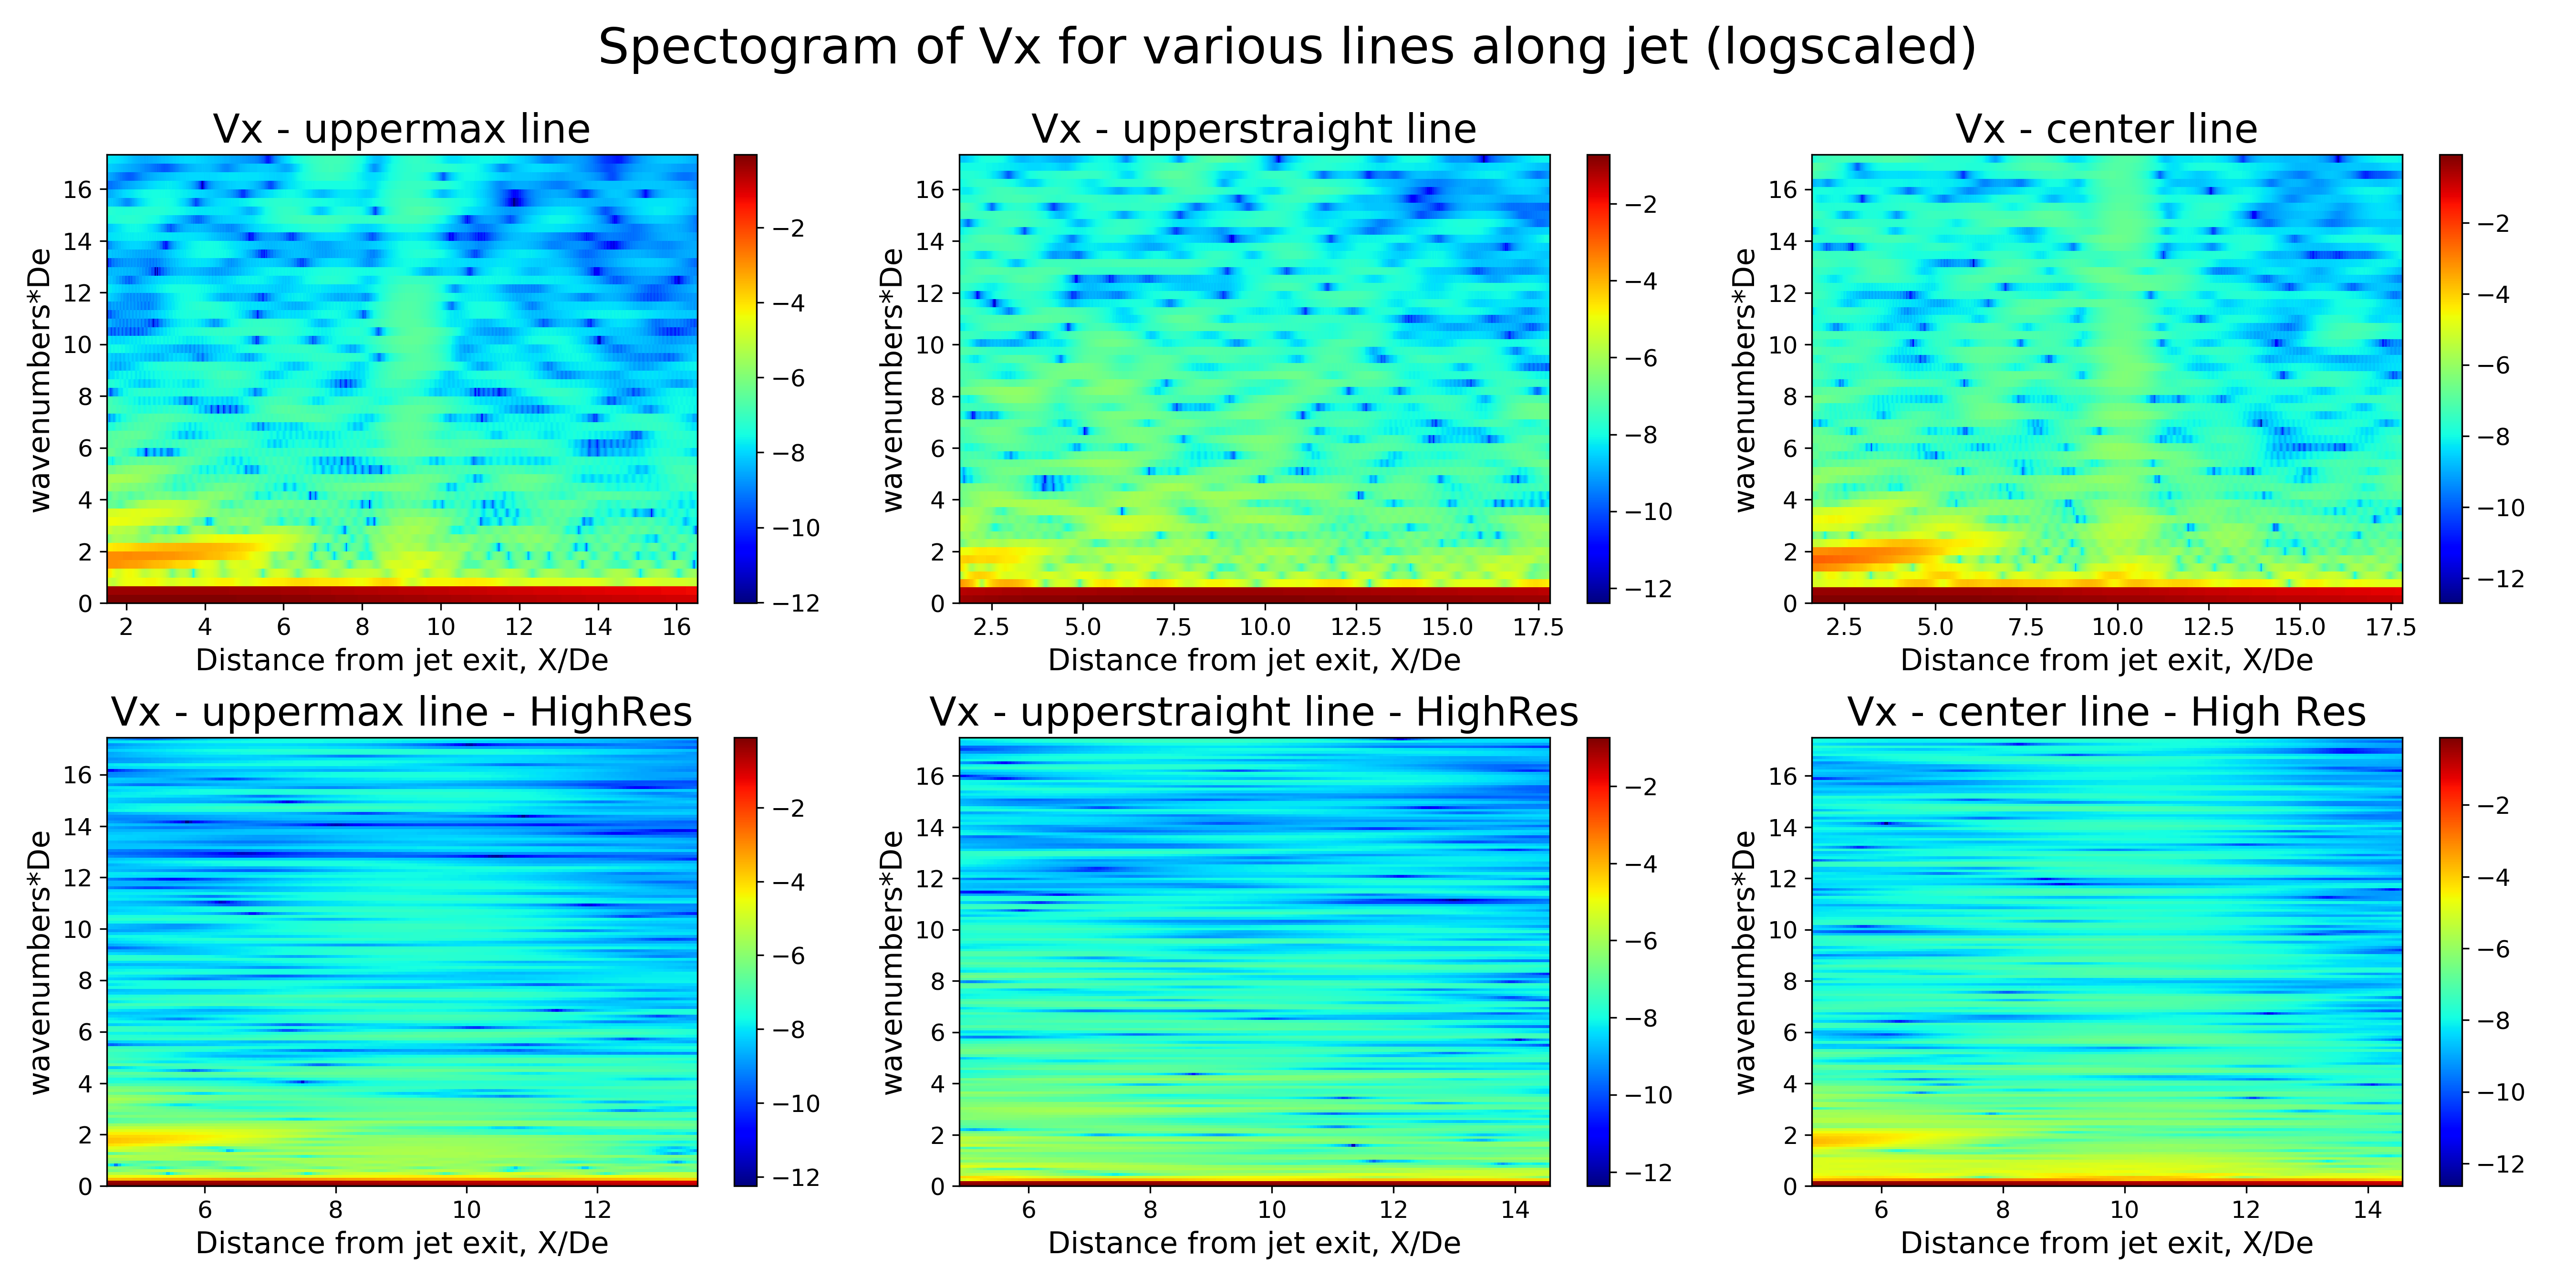
\includegraphics[width=3in]{images/Spectogram_Vx_NTR2p5_NPR2p5.png}
	\caption{NTR:2p5 NPR:2p5 }
	\label{fig:setup1}
\end{subfigure}%
\begin{subfigure}{0.5\textwidth}
	\centering
	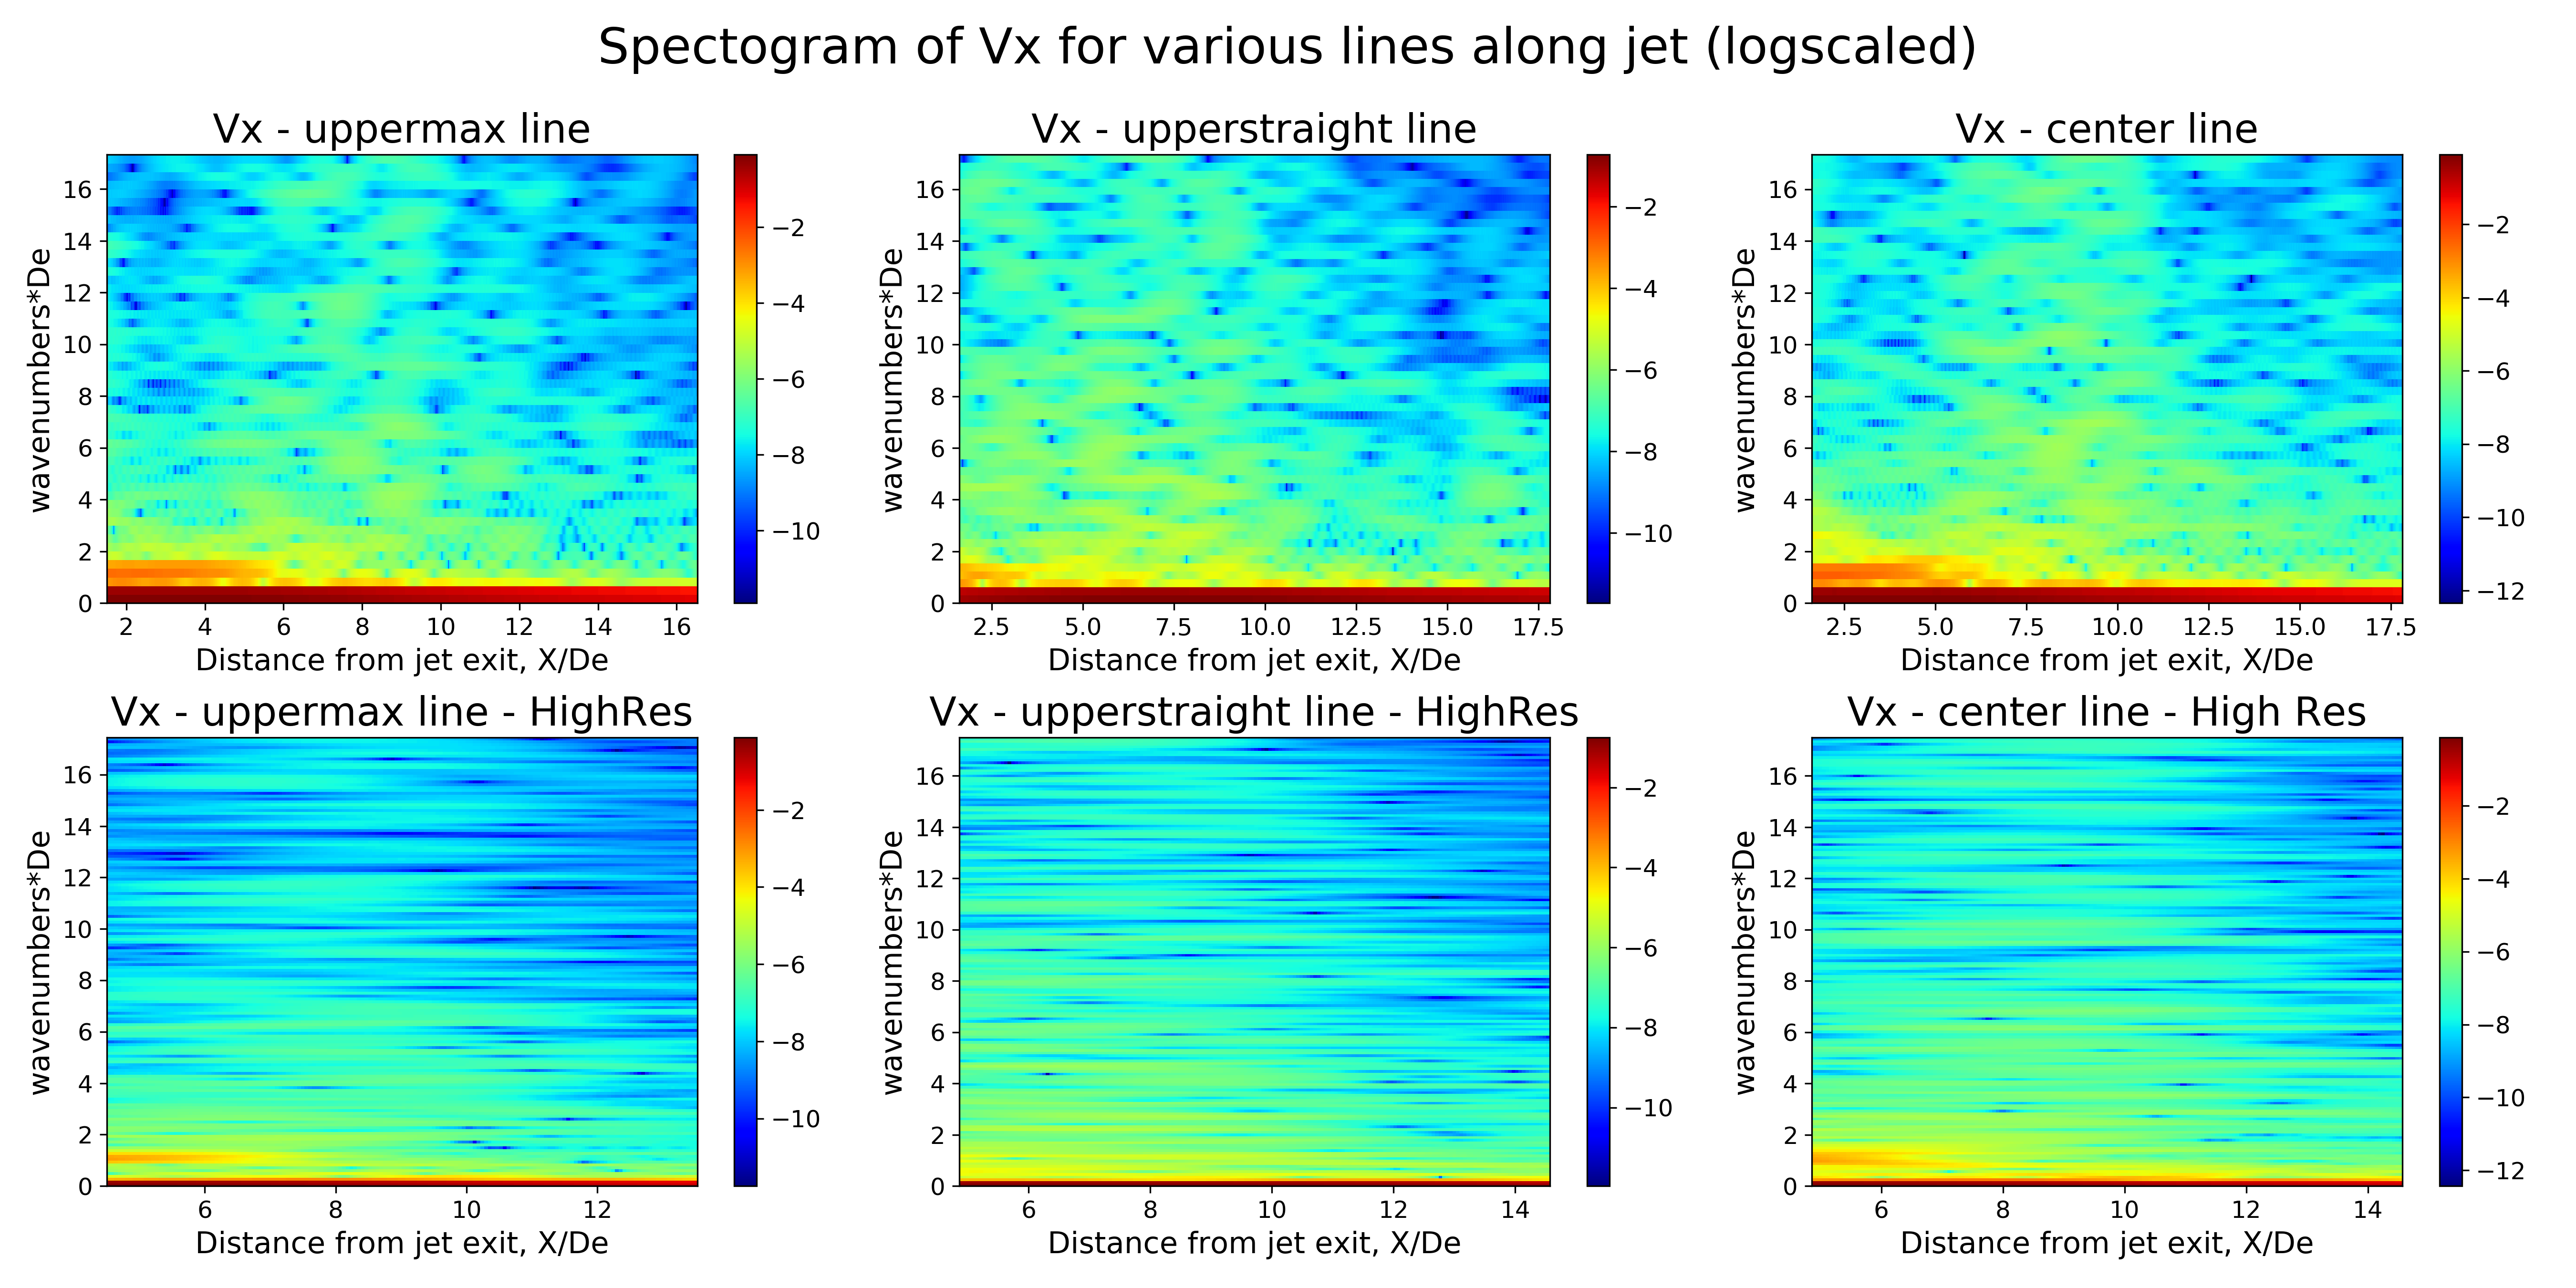
\includegraphics[width=3in]{images/Spectogram_Vx_NTR2p5_NPR3p0.png}
	\caption{NTR:2p5 NPR:3p6 }
	\label{fig:setup2}
\end{subfigure}\\
\begin{subfigure}{0.5\textwidth}
	\centering
	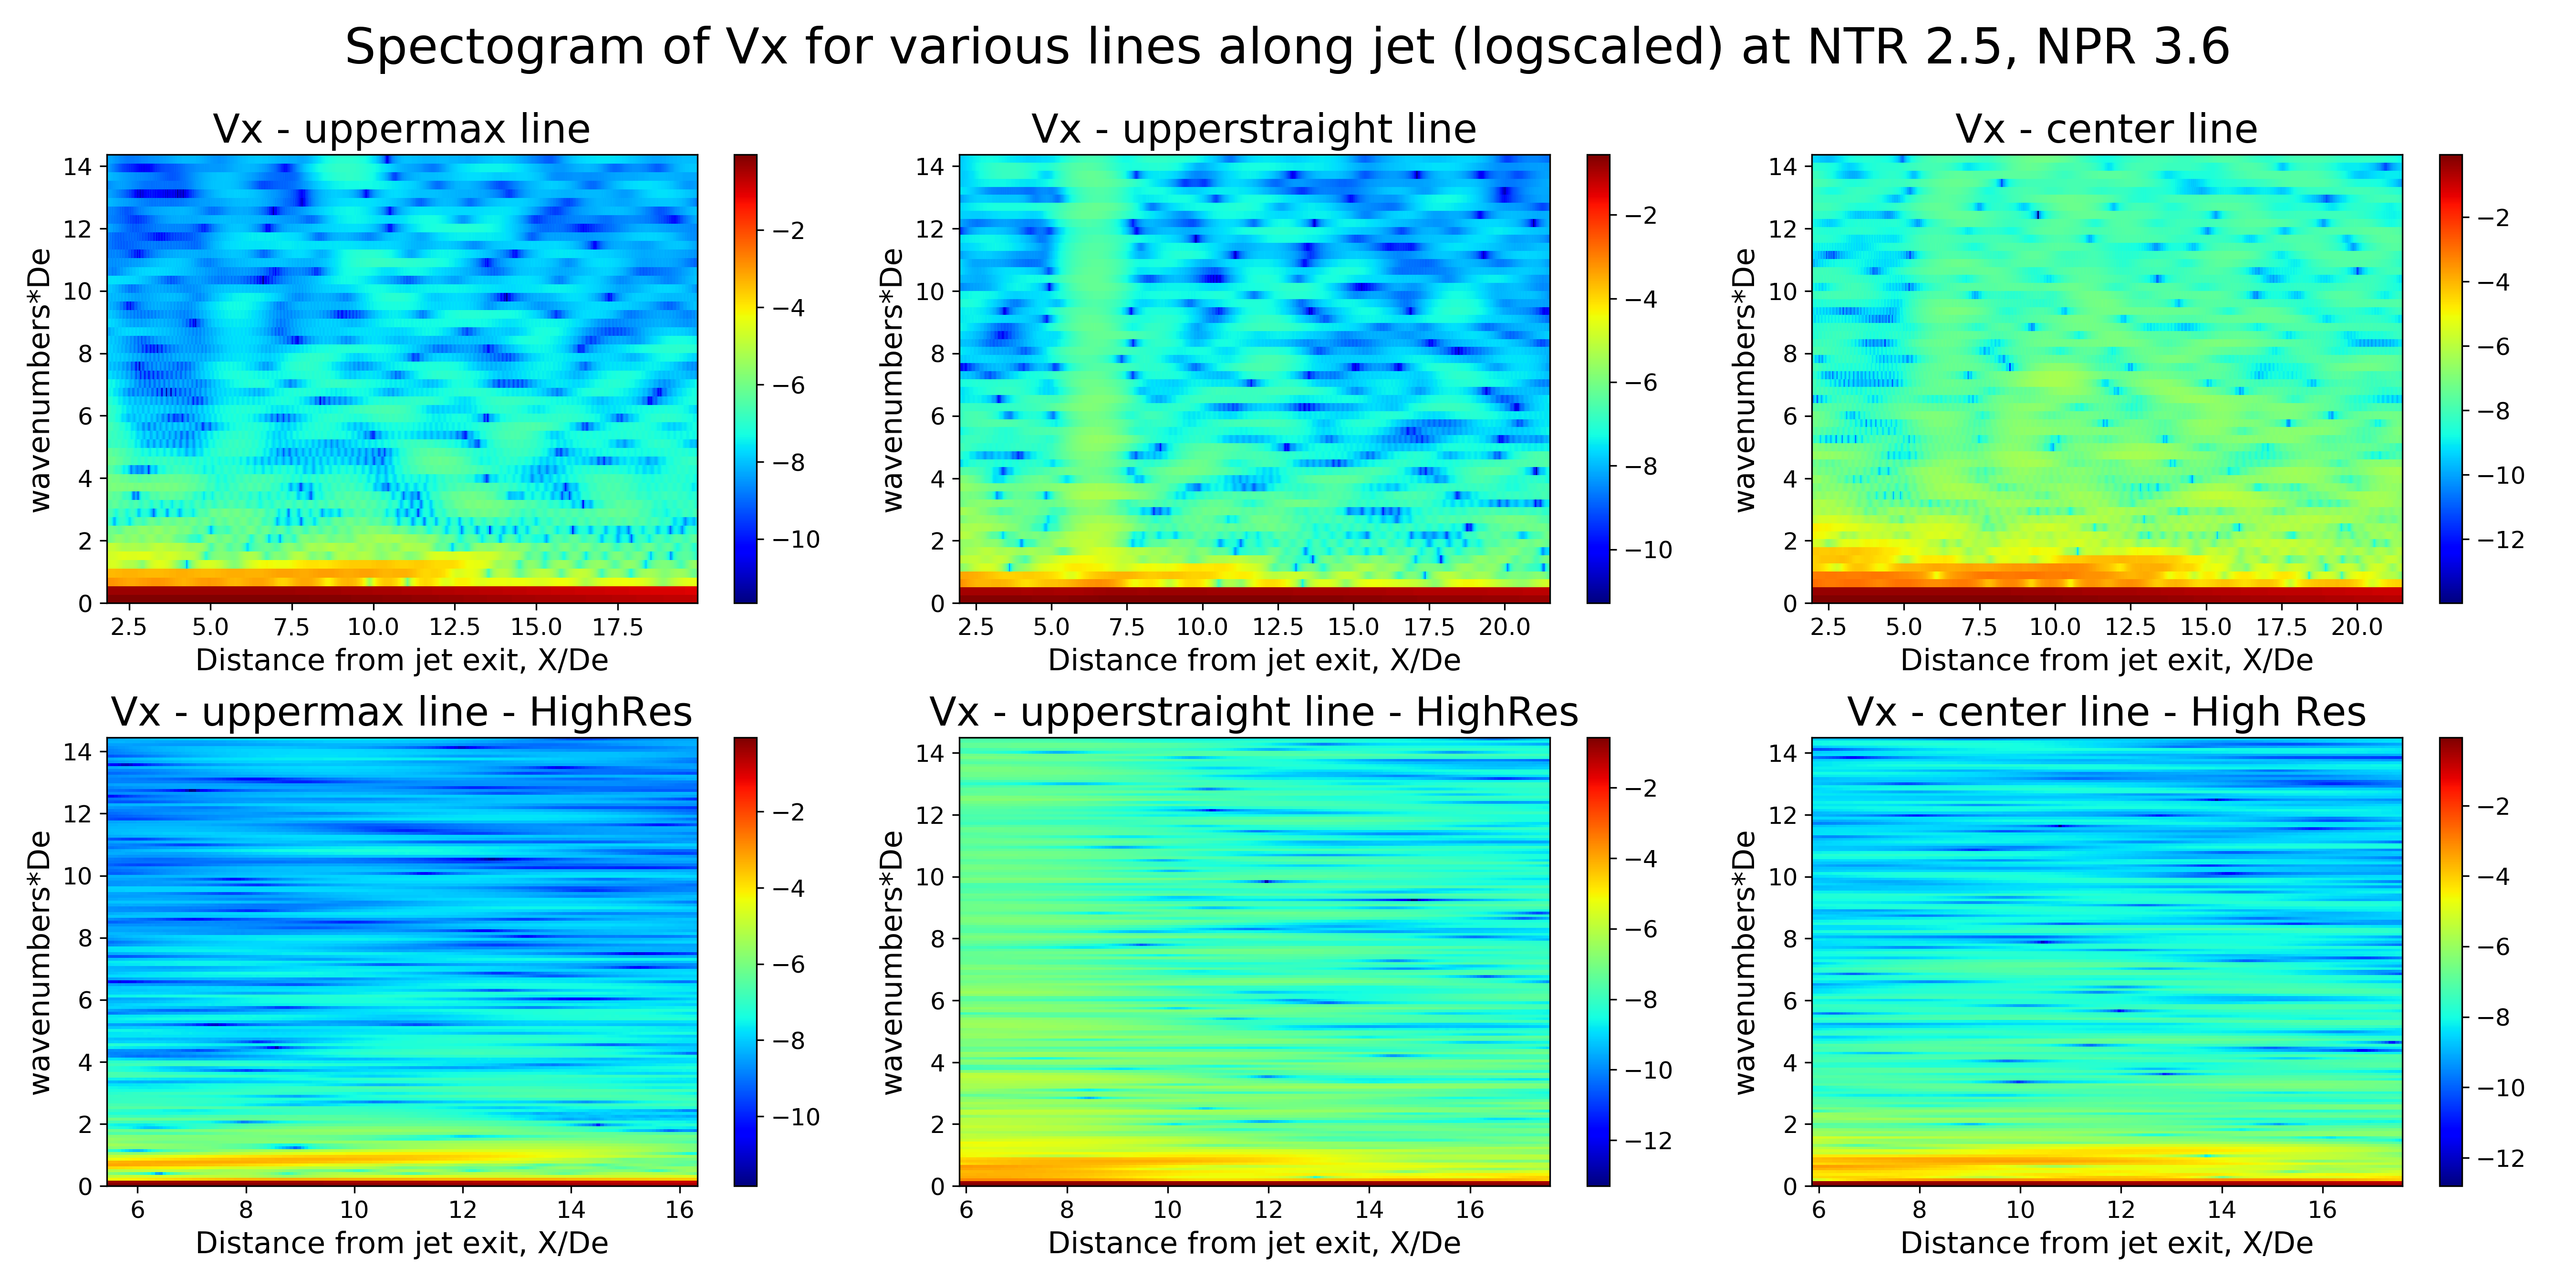
\includegraphics[width=3in]{images/Spectogram_Vx_NTR2p5_NPR3p6.png}
	\caption{NTR:2p5 NPR:2p5 }
	\label{fig:setup1}
\end{subfigure}%
\begin{subfigure}{0.5\textwidth}
	\centering
	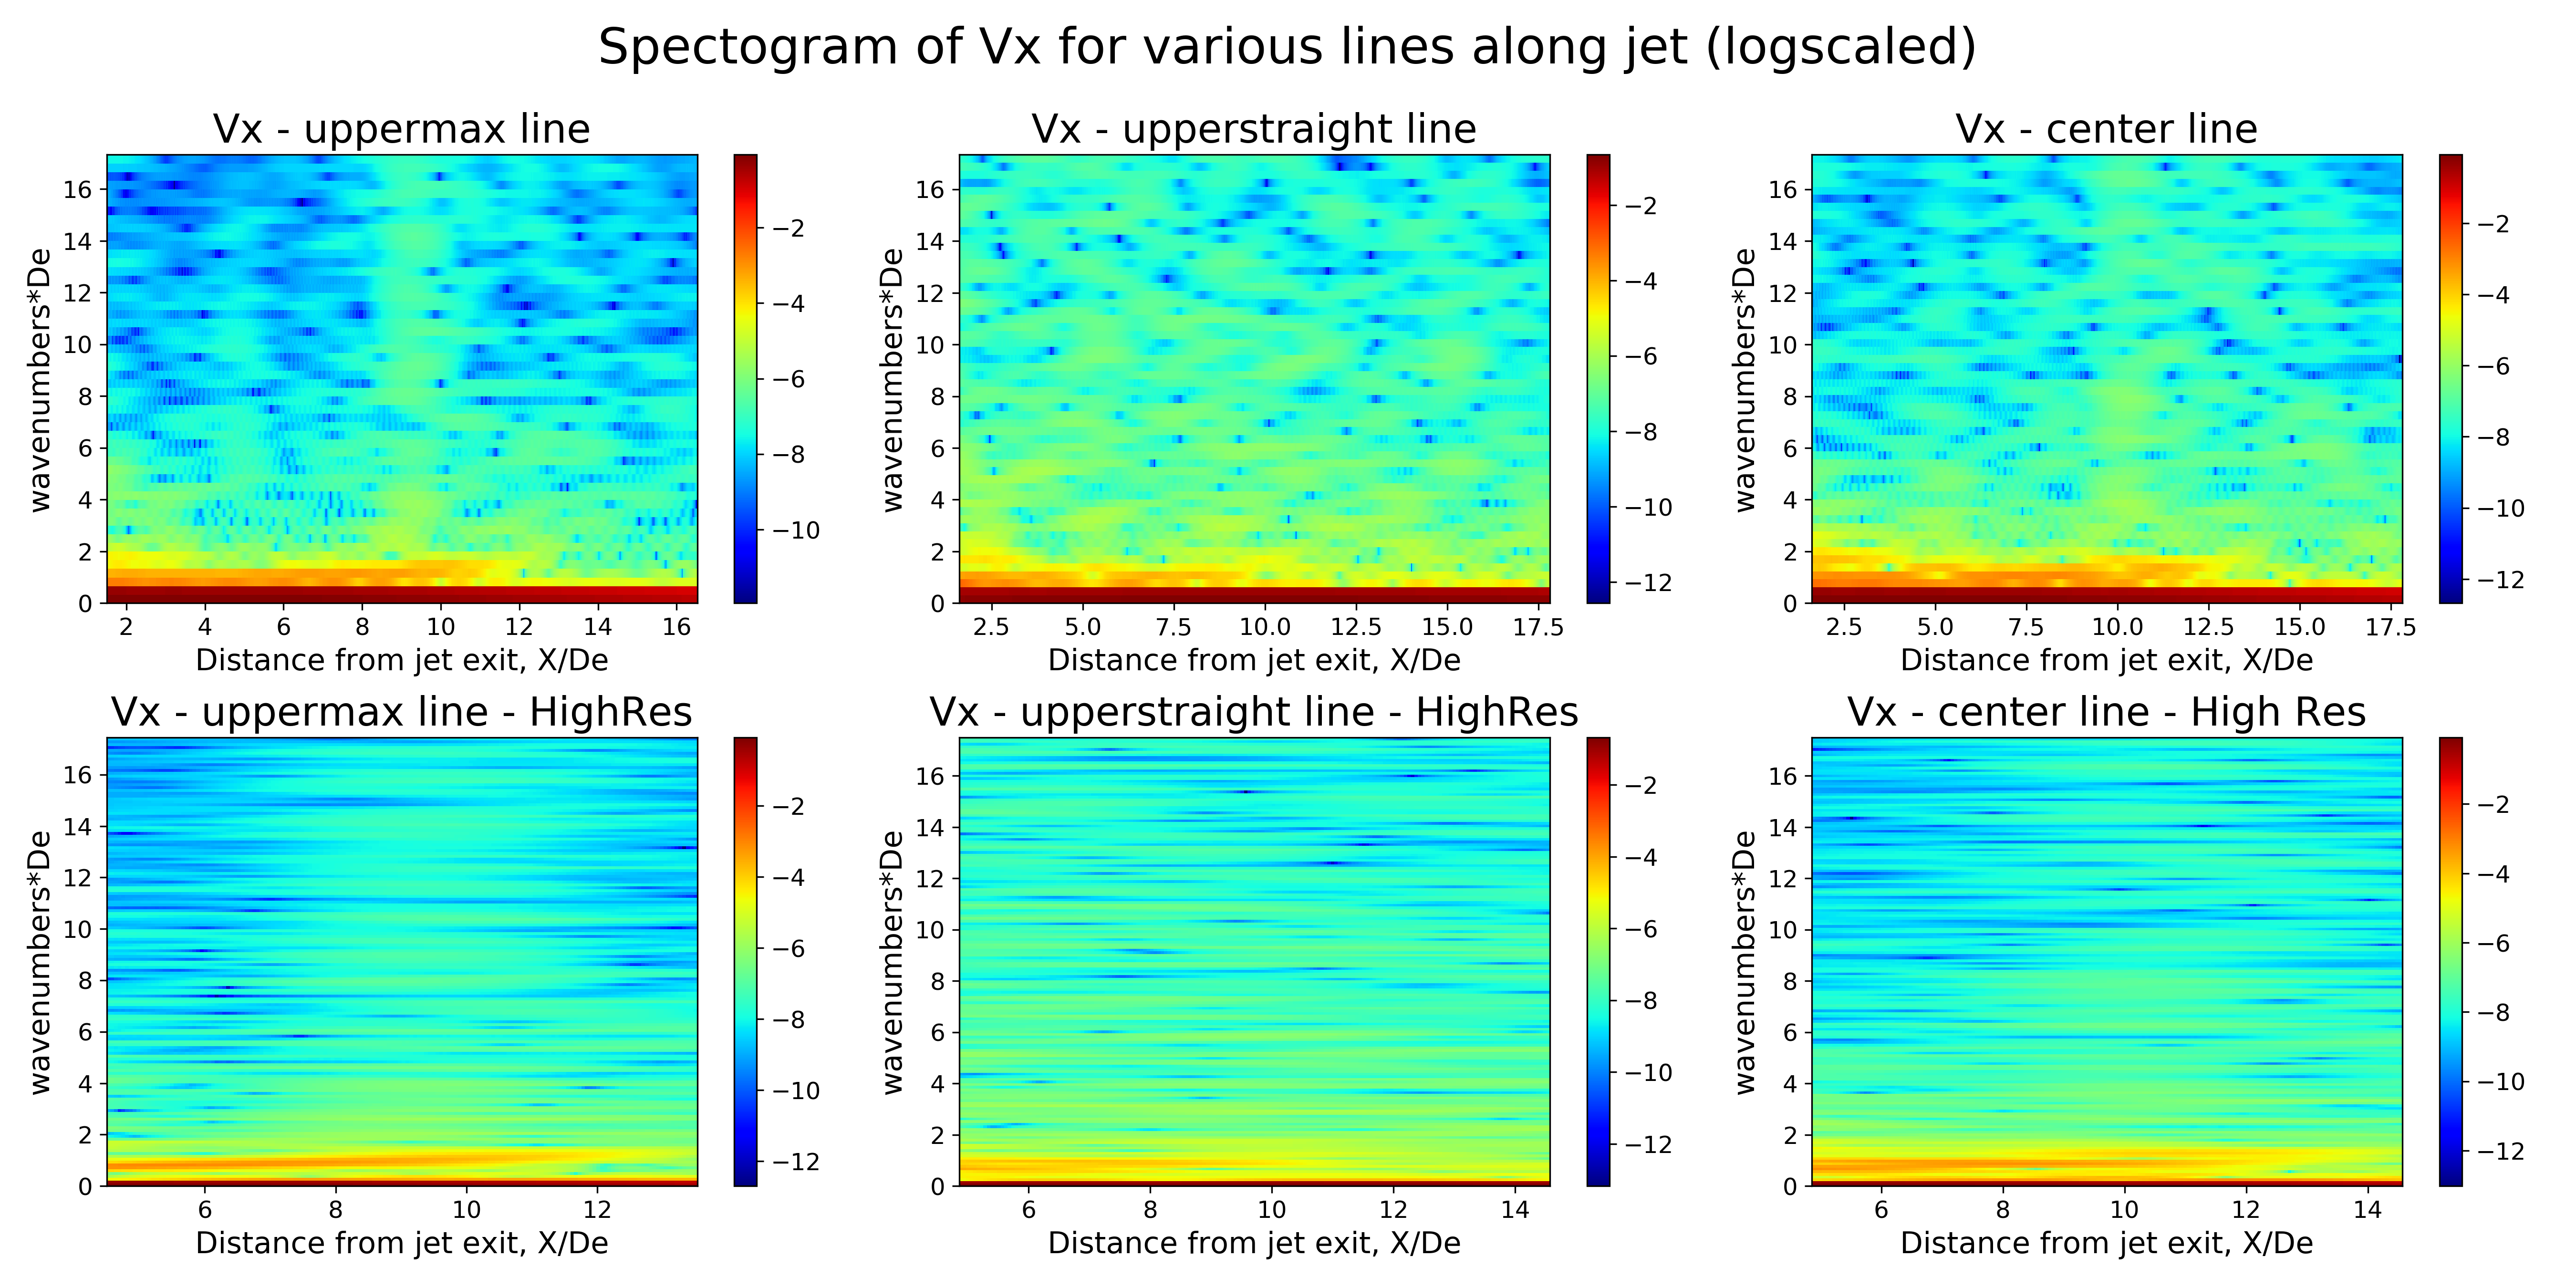
\includegraphics[width=3in]{images/Spectogram_Vx_NTR2p5_NPR4p0.png}
	\caption{NTR:2p5 NPR:3p6 }
	\label{fig:setup2}
\end{subfigure}
\caption{Spectogram plots for centreline $V_x$ without chevrons }
\label{fig:spectogramVx}
\end{figure} 

\begin{figure}[H]
\begin{subfigure}{0.5\textwidth}
	\centering
	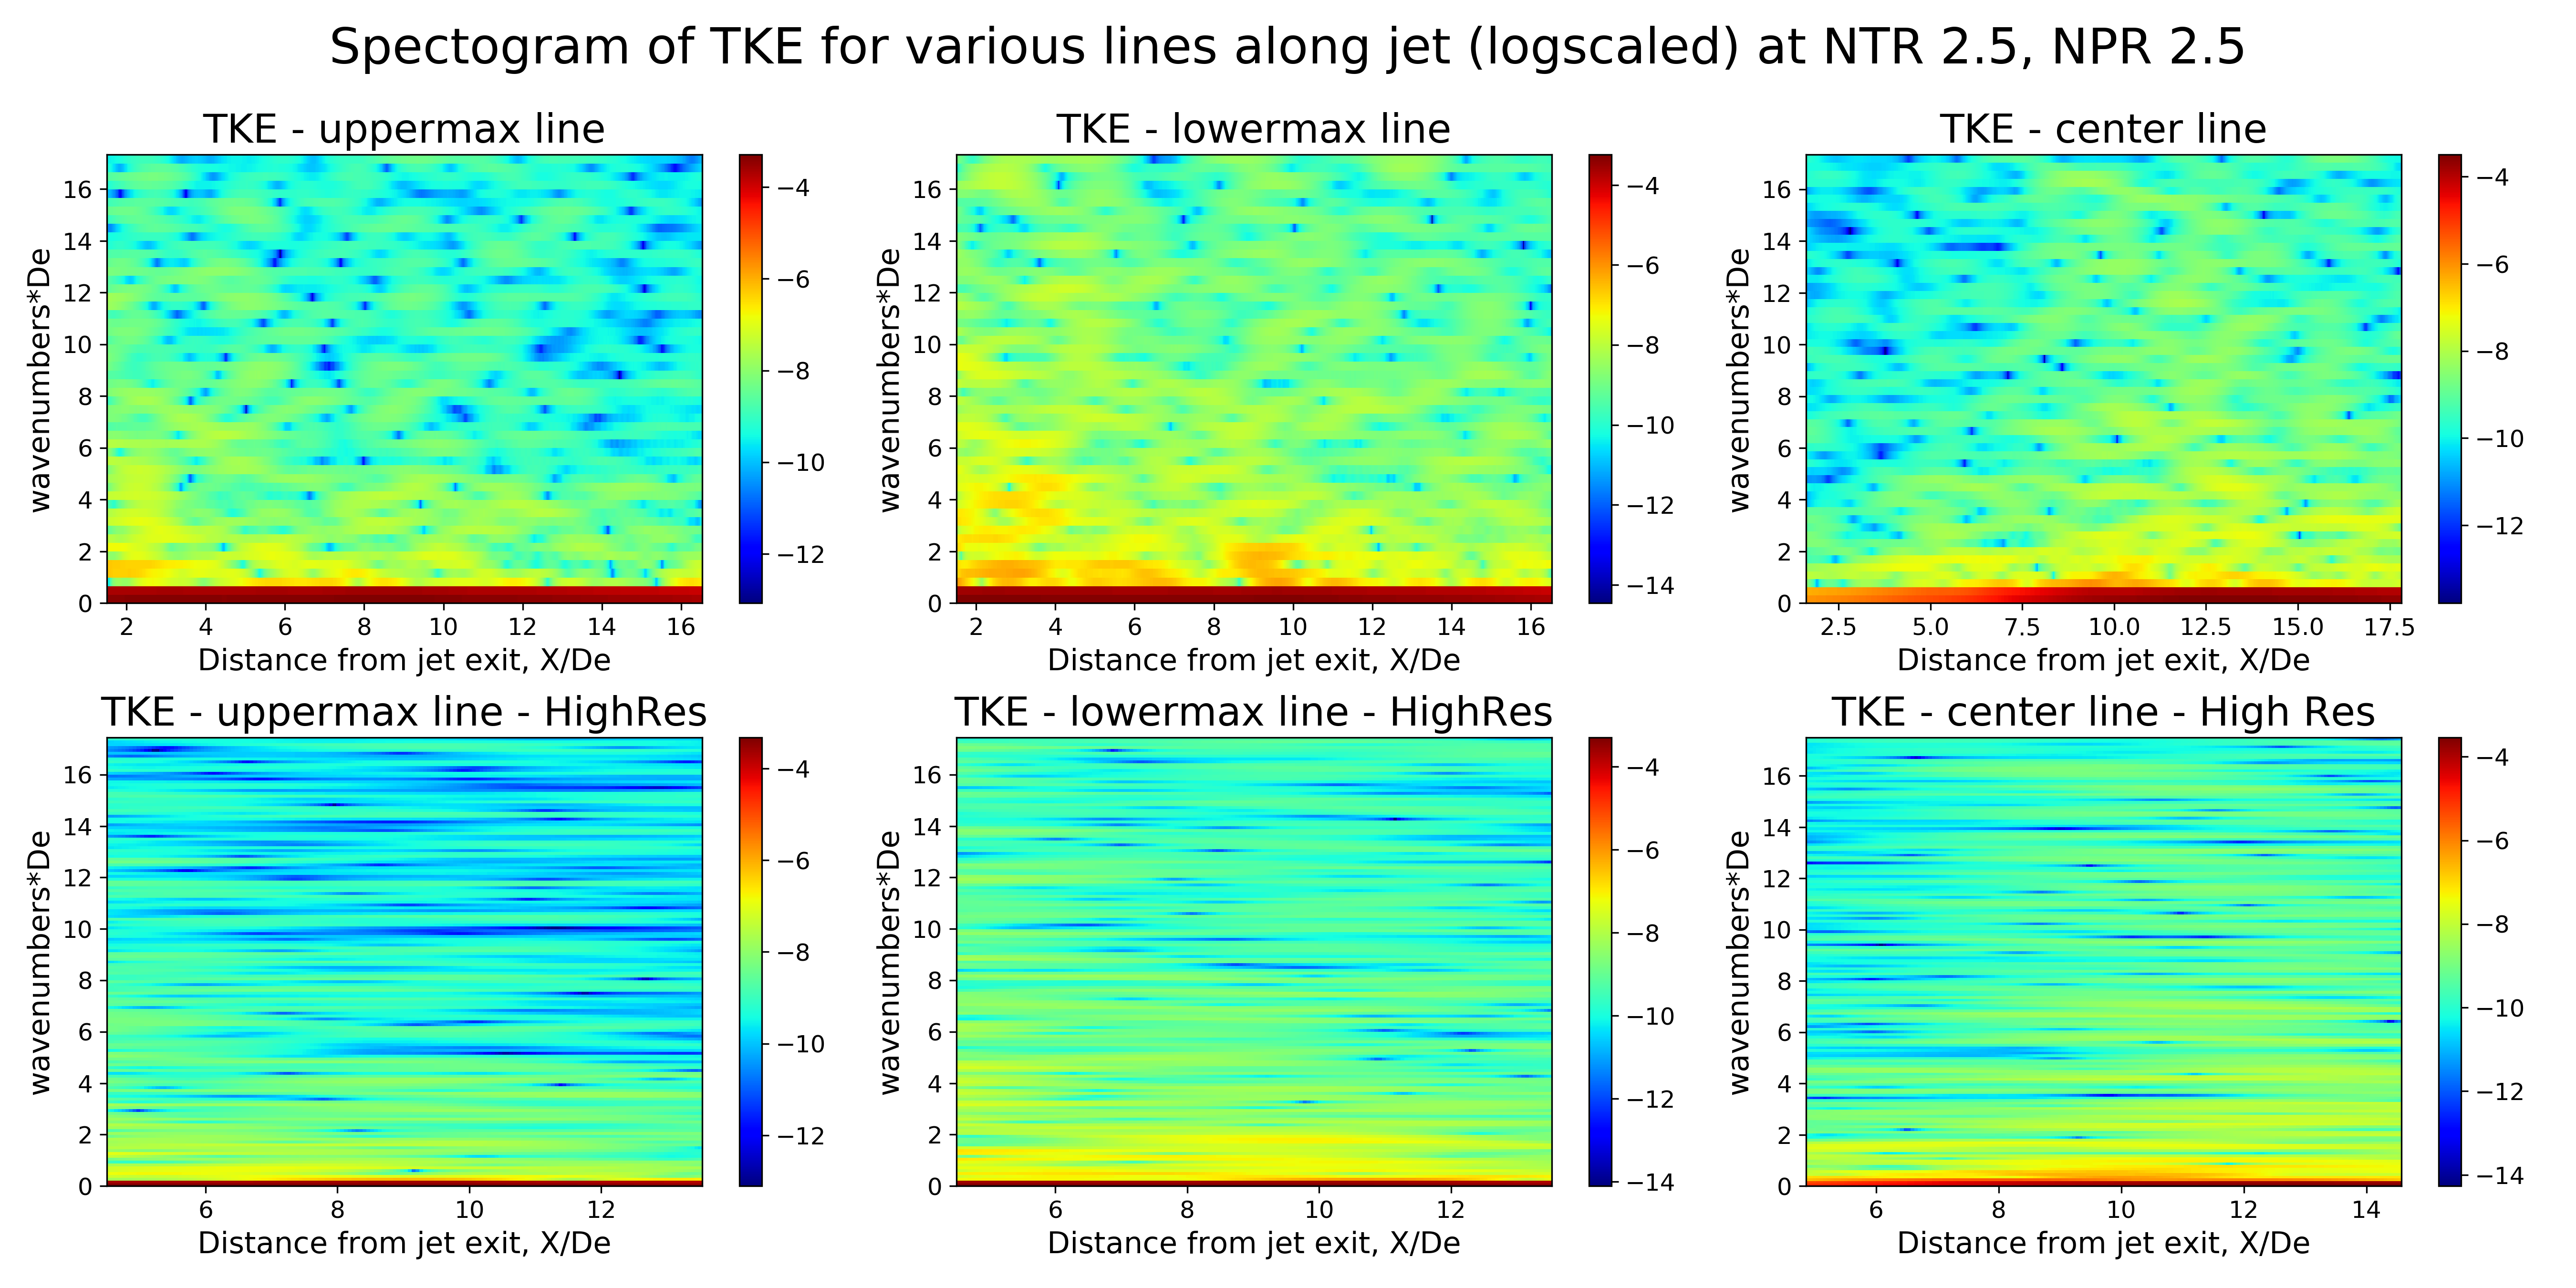
\includegraphics[width=3in]{images/Spectogram_TKE_NTR2p5_NPR2p5.png}
	\caption{NTR:2p5 NPR:2p5 }
	\label{fig:setup1}
\end{subfigure}%
\begin{subfigure}{0.5\textwidth}
	\centering
	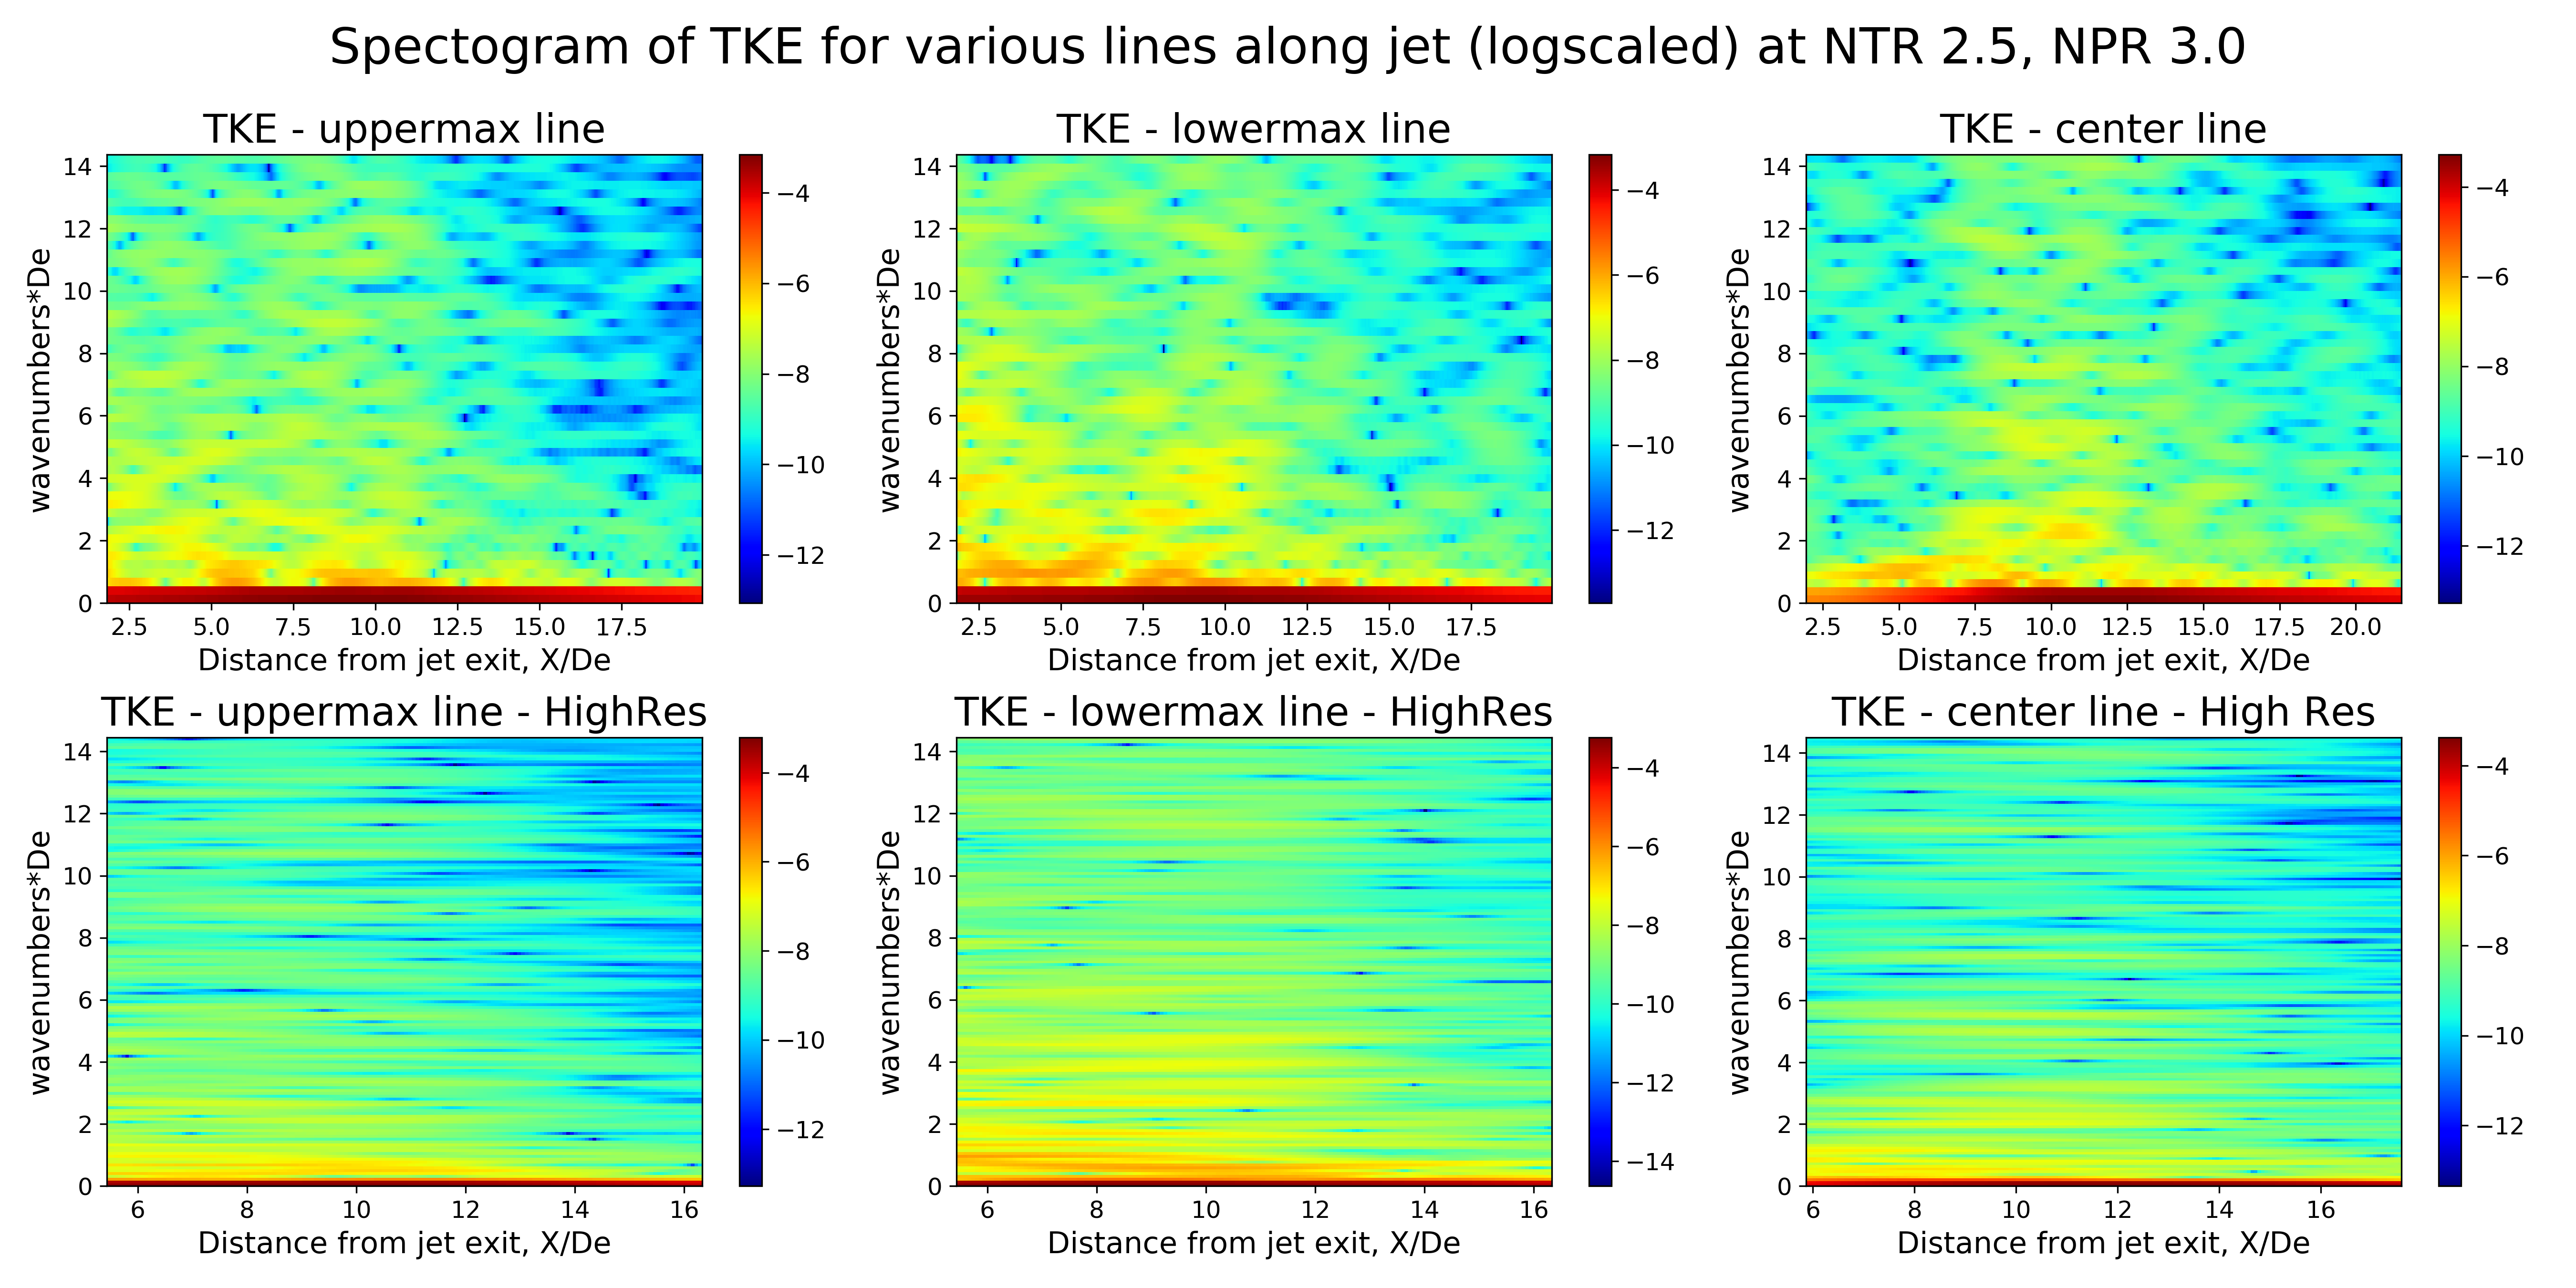
\includegraphics[width=3in]{images/Spectogram_TKE_NTR2p5_NPR3p0.png}
	\caption{NTR:2p5 NPR:3p6 }
	\label{fig:setup2}
\end{subfigure}\\
\begin{subfigure}{0.5\textwidth}
	\centering
	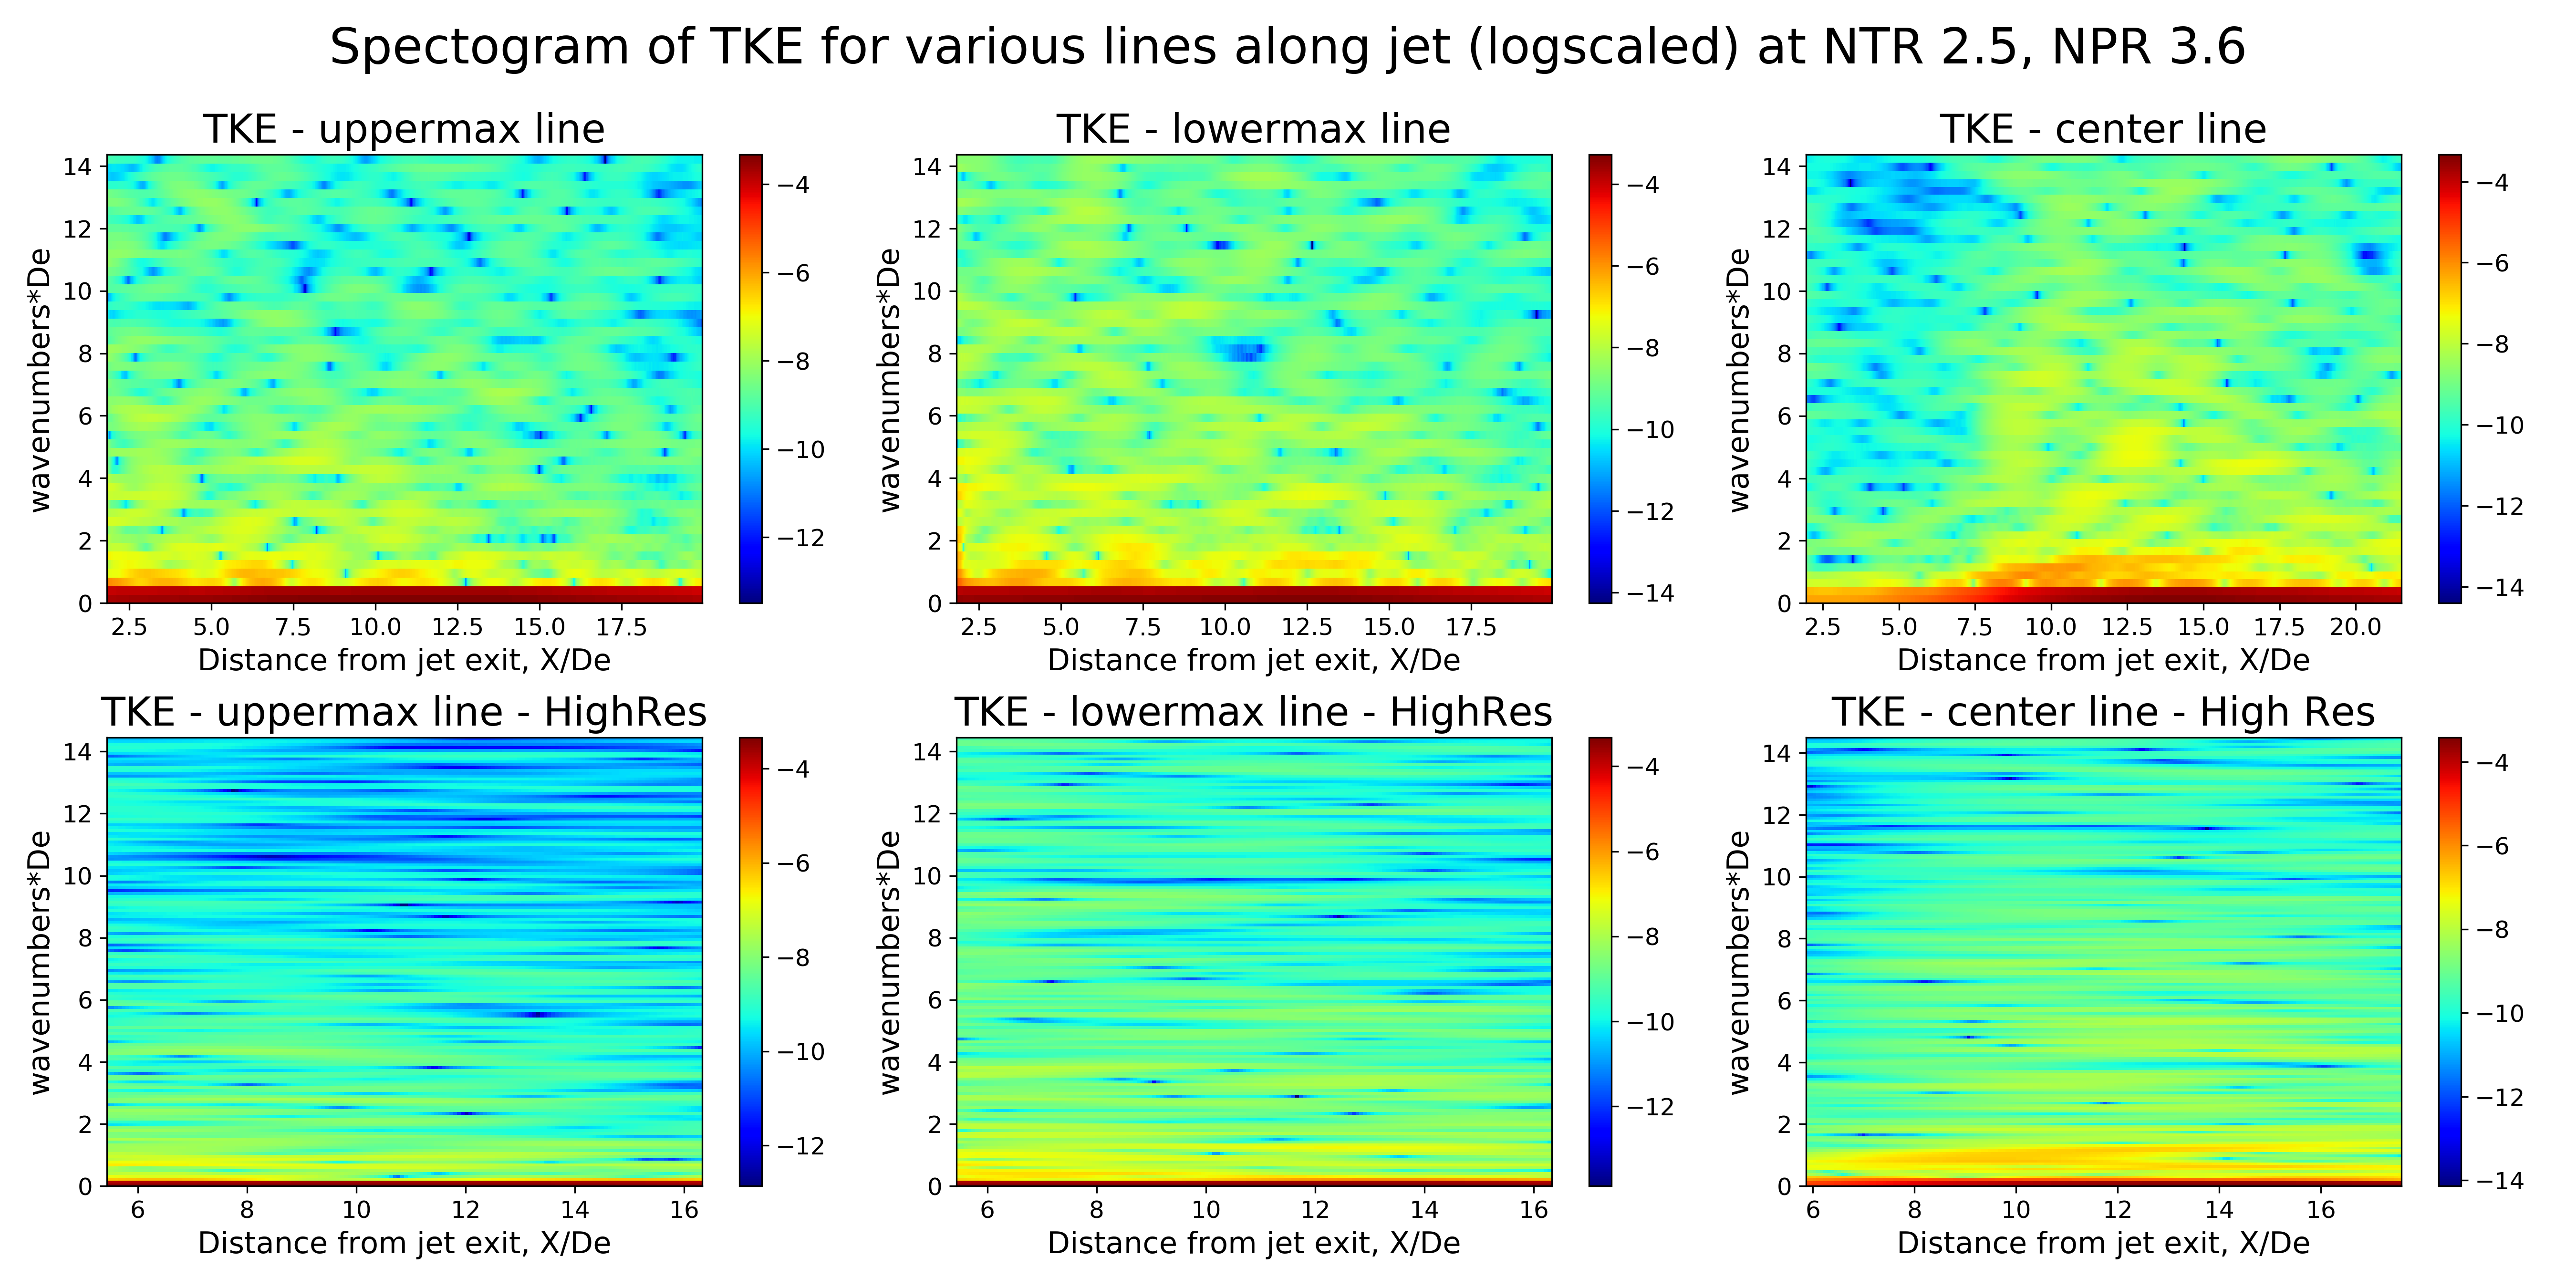
\includegraphics[width=3in]{images/Spectogram_TKE_NTR2p5_NPR3p6.png}
	\caption{NTR:2p5 NPR:2p5 }
	\label{fig:setup1}
\end{subfigure}%
\begin{subfigure}{0.5\textwidth}
	\centering
	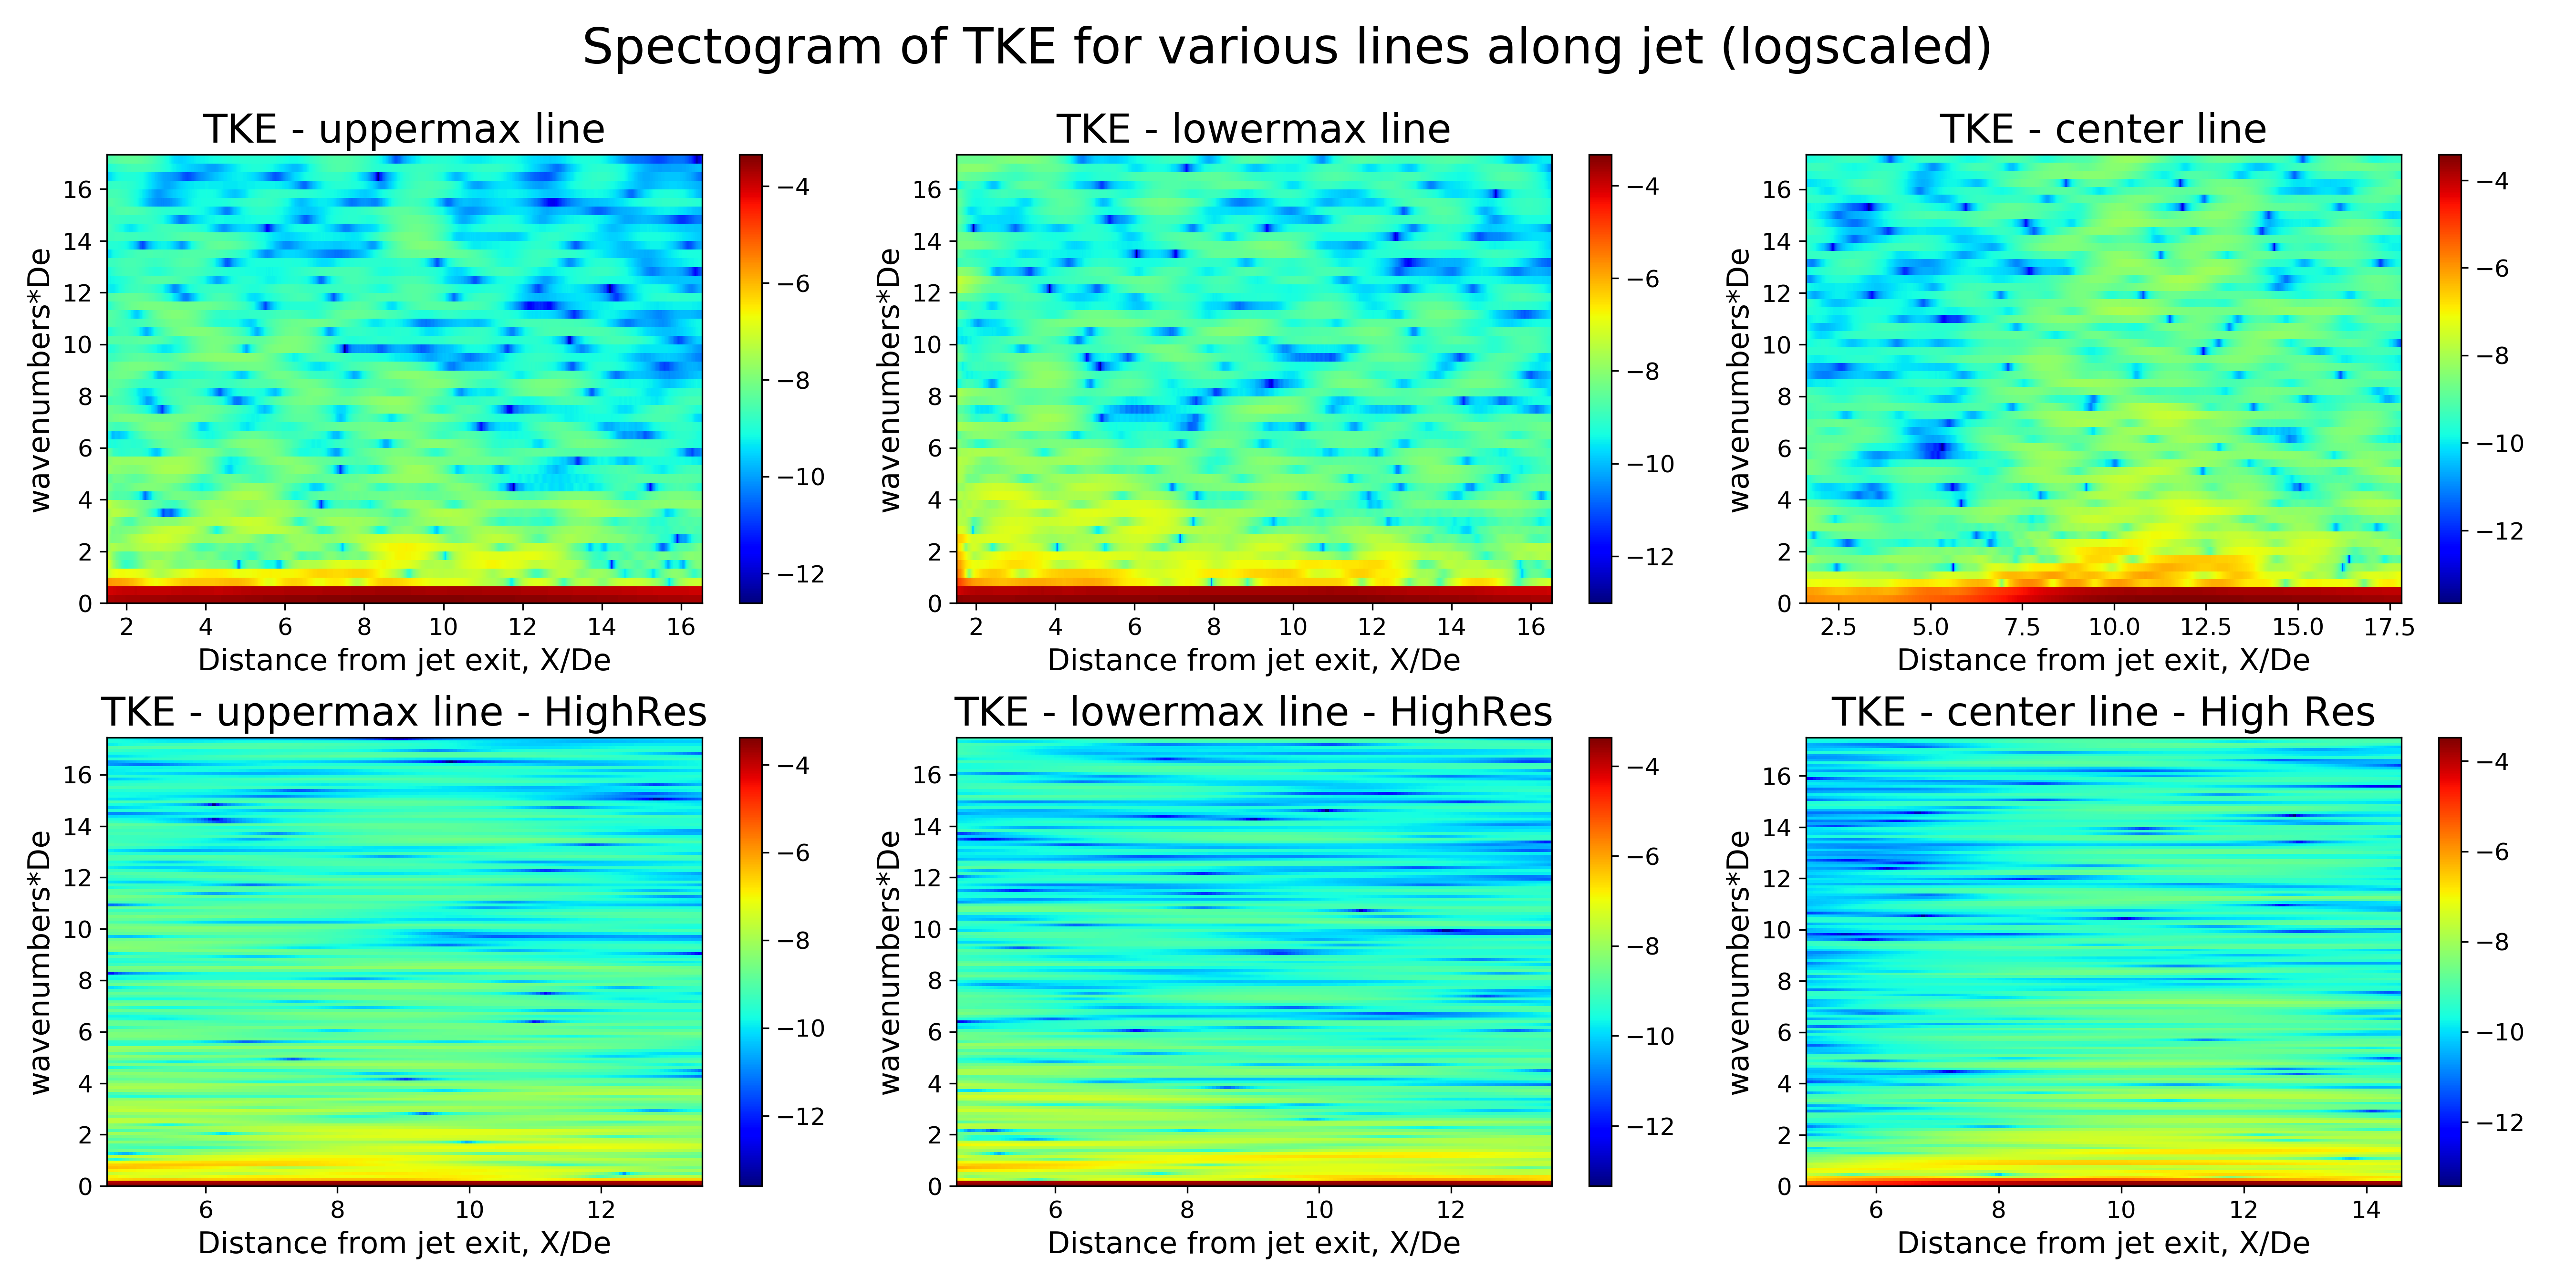
\includegraphics[width=3in]{images/Spectogram_TKE_NTR2p5_NPR4p0.png}
	\caption{NTR:2p5 NPR:3p6 }
	\label{fig:setup2}
\end{subfigure}
\caption{Spectogram plots for centreline TKE without chevrons }
\label{fig:spectogramTKE}
\end{figure} 

\section{Effect of Chevron}  

Only three cases, all perfectly expanded flows for different temperatures, have been studied with chevrons. Fig shows that the temperature doesn't affect the wavelength value but clearly reducing the intensity of pattern as seen before without chevrons. Also, we can notice that now the wavelength is about 25-30\% less than the values obtained without chevrons. This shows that chevrons are decreasing the length of shock cells, perhaps by increasing mixing between layers. This is as expected from the discussion in Heeb et.al.\cite{heeb} which is the reason BBSN tends to shift towards higher frequency. From fig \ref{fig:lineplotsTKE}, Point of merging of centreline plots  with lines at lips is closer to exit at each temperature implying the decrease in potential core length. Also, increase in temperature decreases potential core length for both with and without chevrons. 

\begin{figure}[H]
\begin{subfigure}{.5\textwidth}
	\centering
	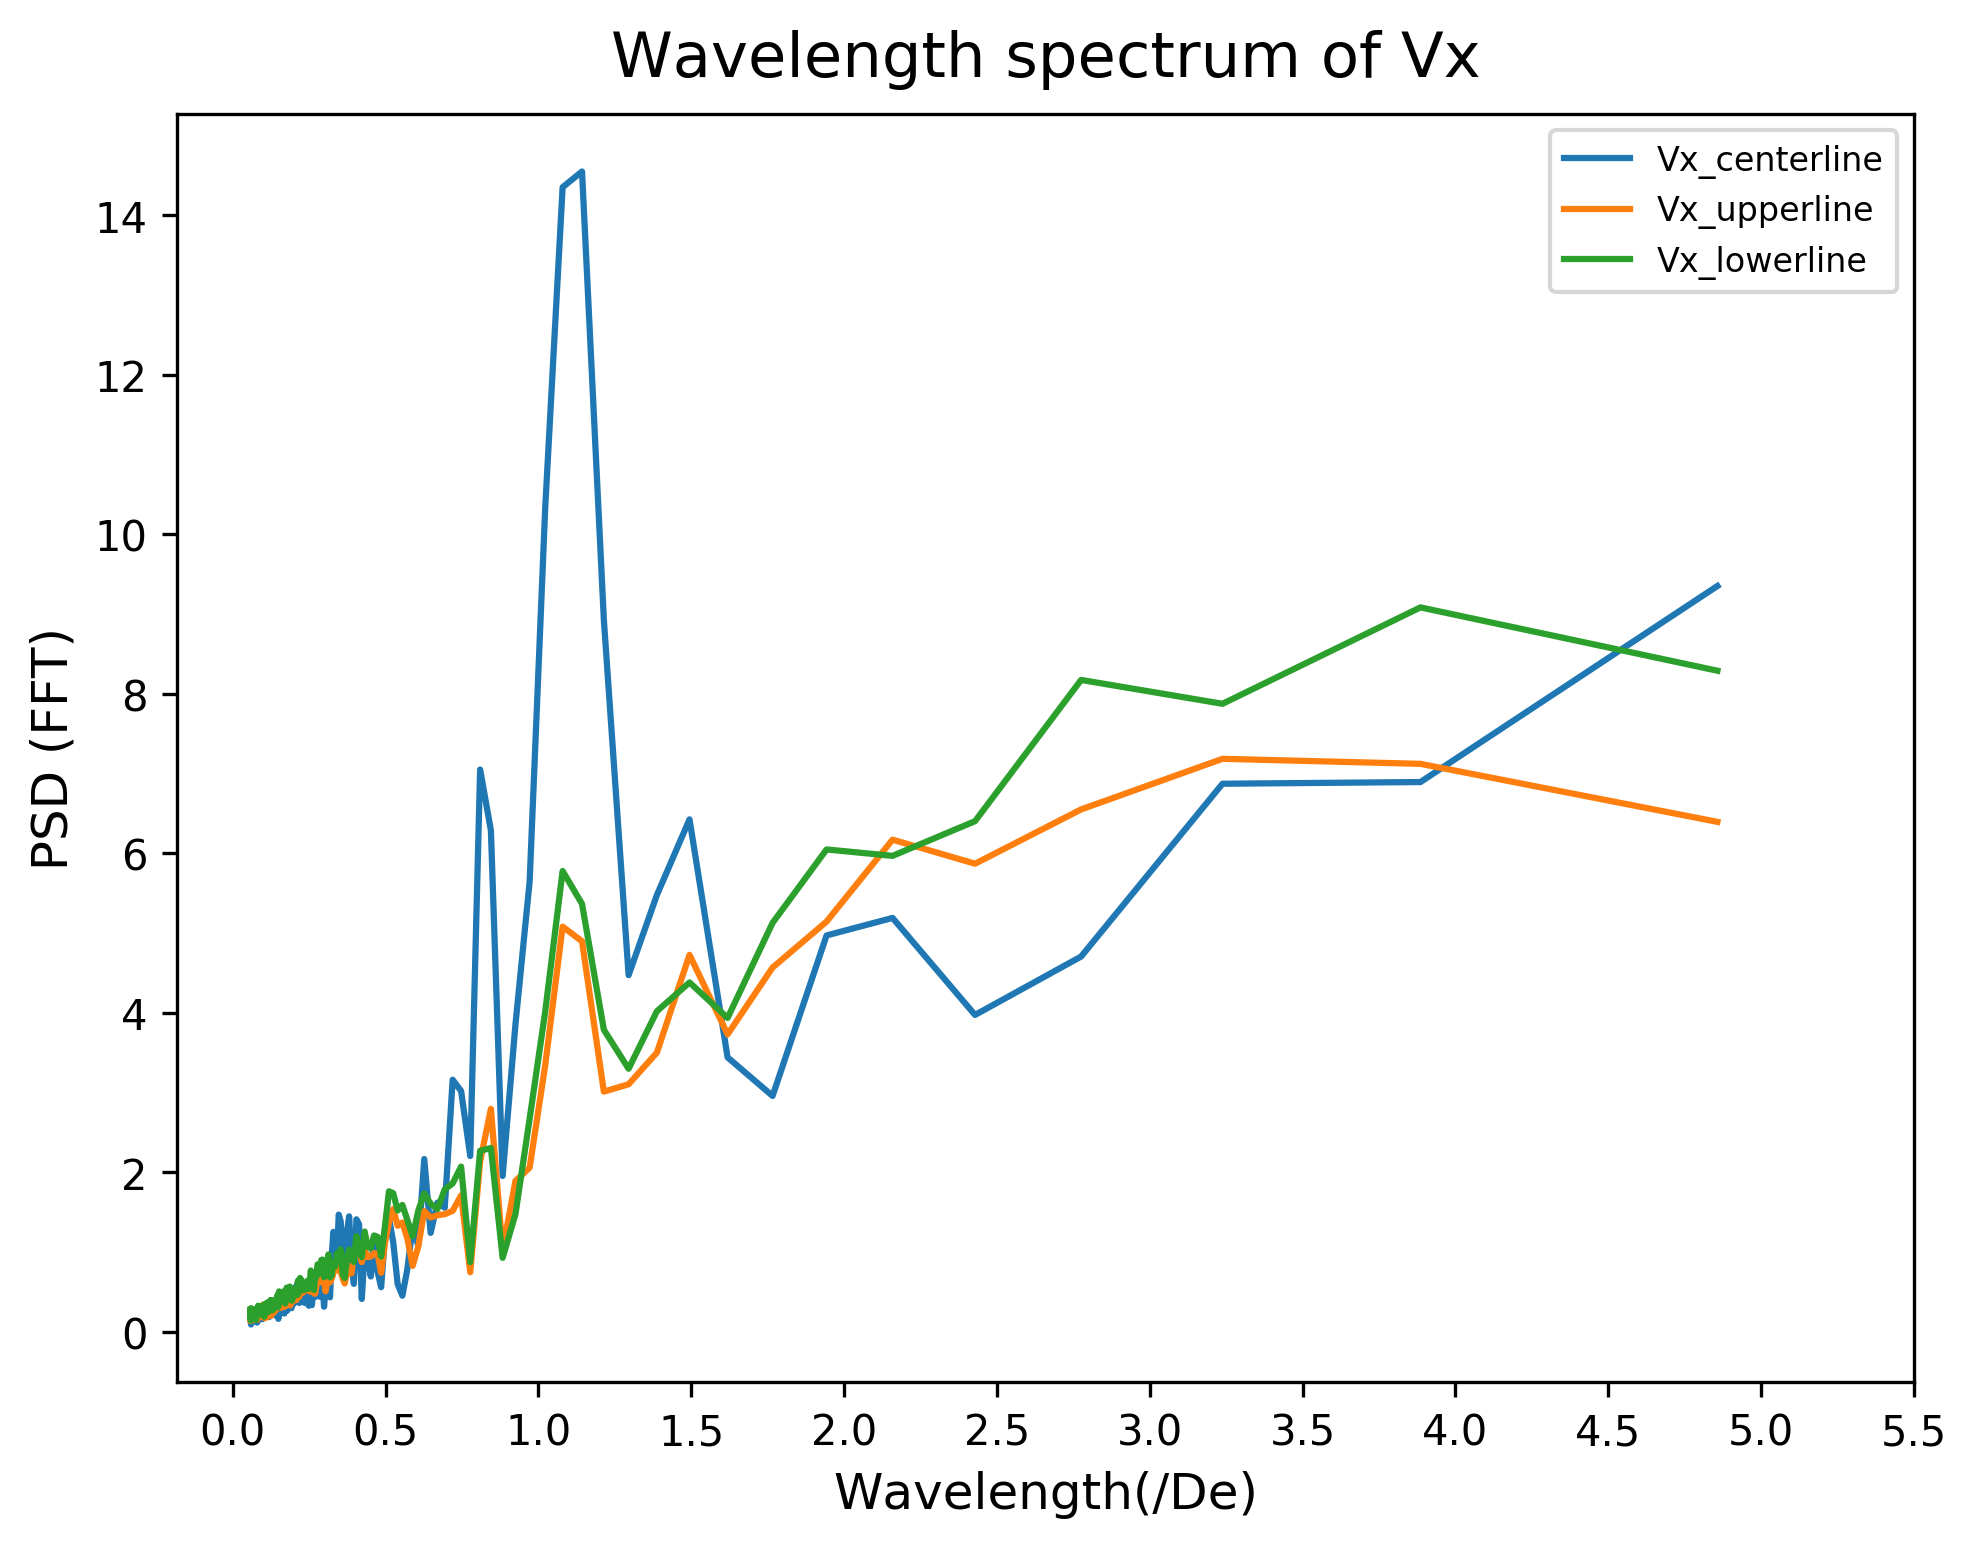
\includegraphics[width=3in]{images/Fft_Vx_NTR1p0_NPR3p6c.png}
	\caption{NTR:1p0 NPR:3p6 with chevrons }
	\label{fig:setup1}
\end{subfigure}%
\begin{subfigure}{.5\textwidth}
	\centering
	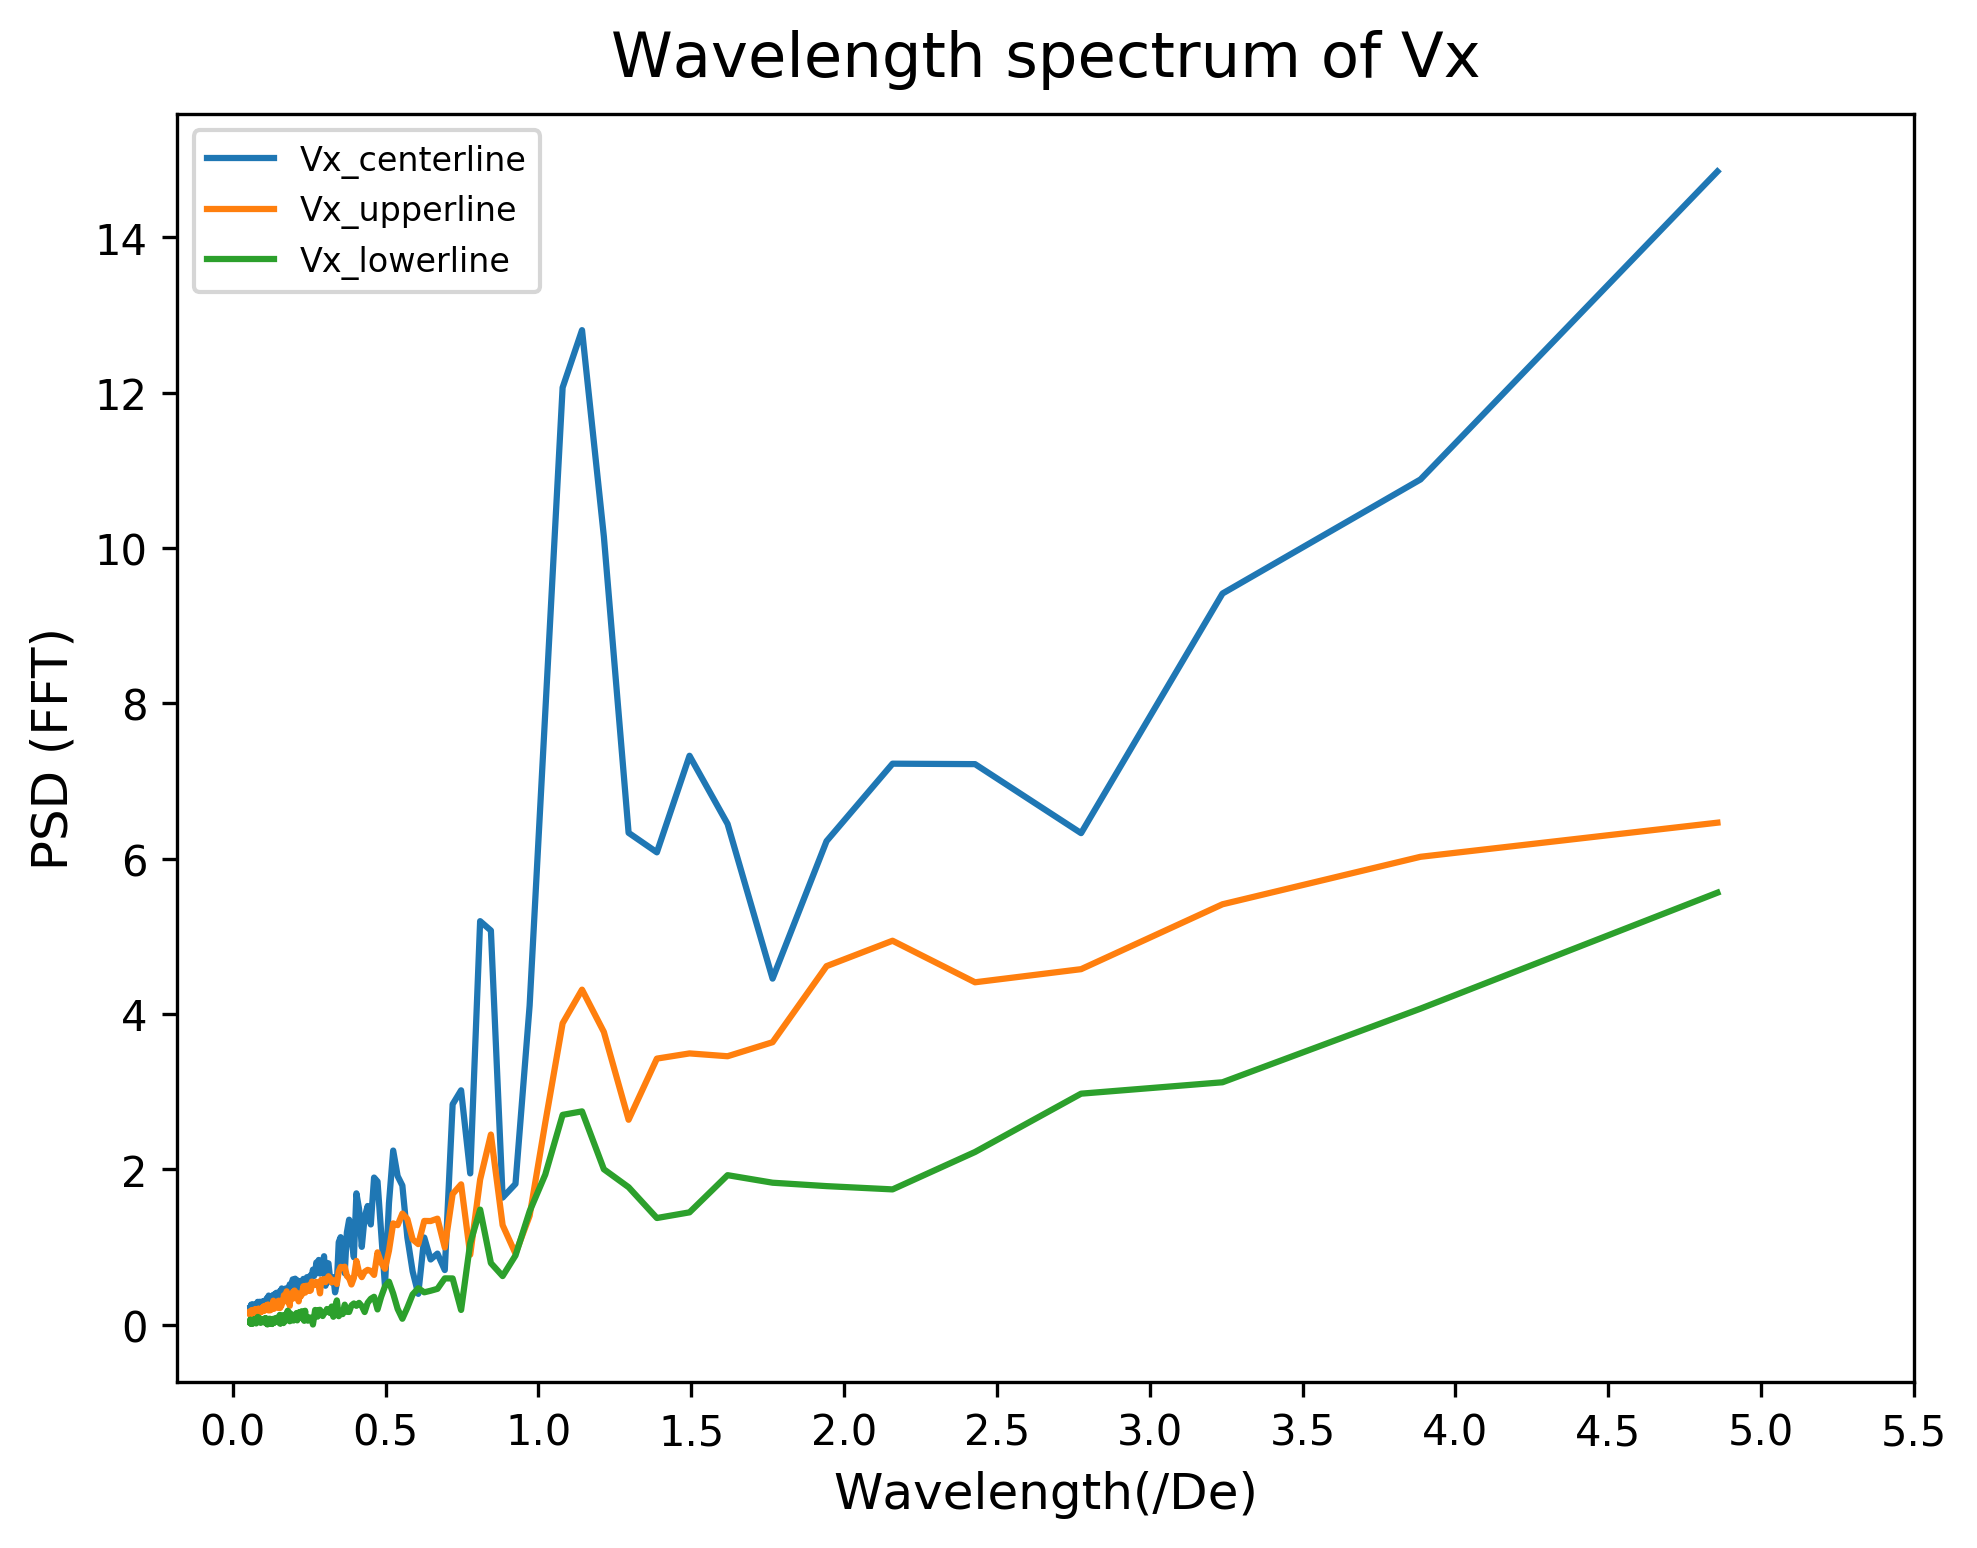
\includegraphics[width=3in]{images/Fft_Vx_NTR2p0_NPR3p6c.png}
	\caption{NTR:2p0 NPR:3p6 with chevrons}
	\label{fig:setup2}
\end{subfigure}
\begin{subfigure}{1.0\textwidth}
	\centering
	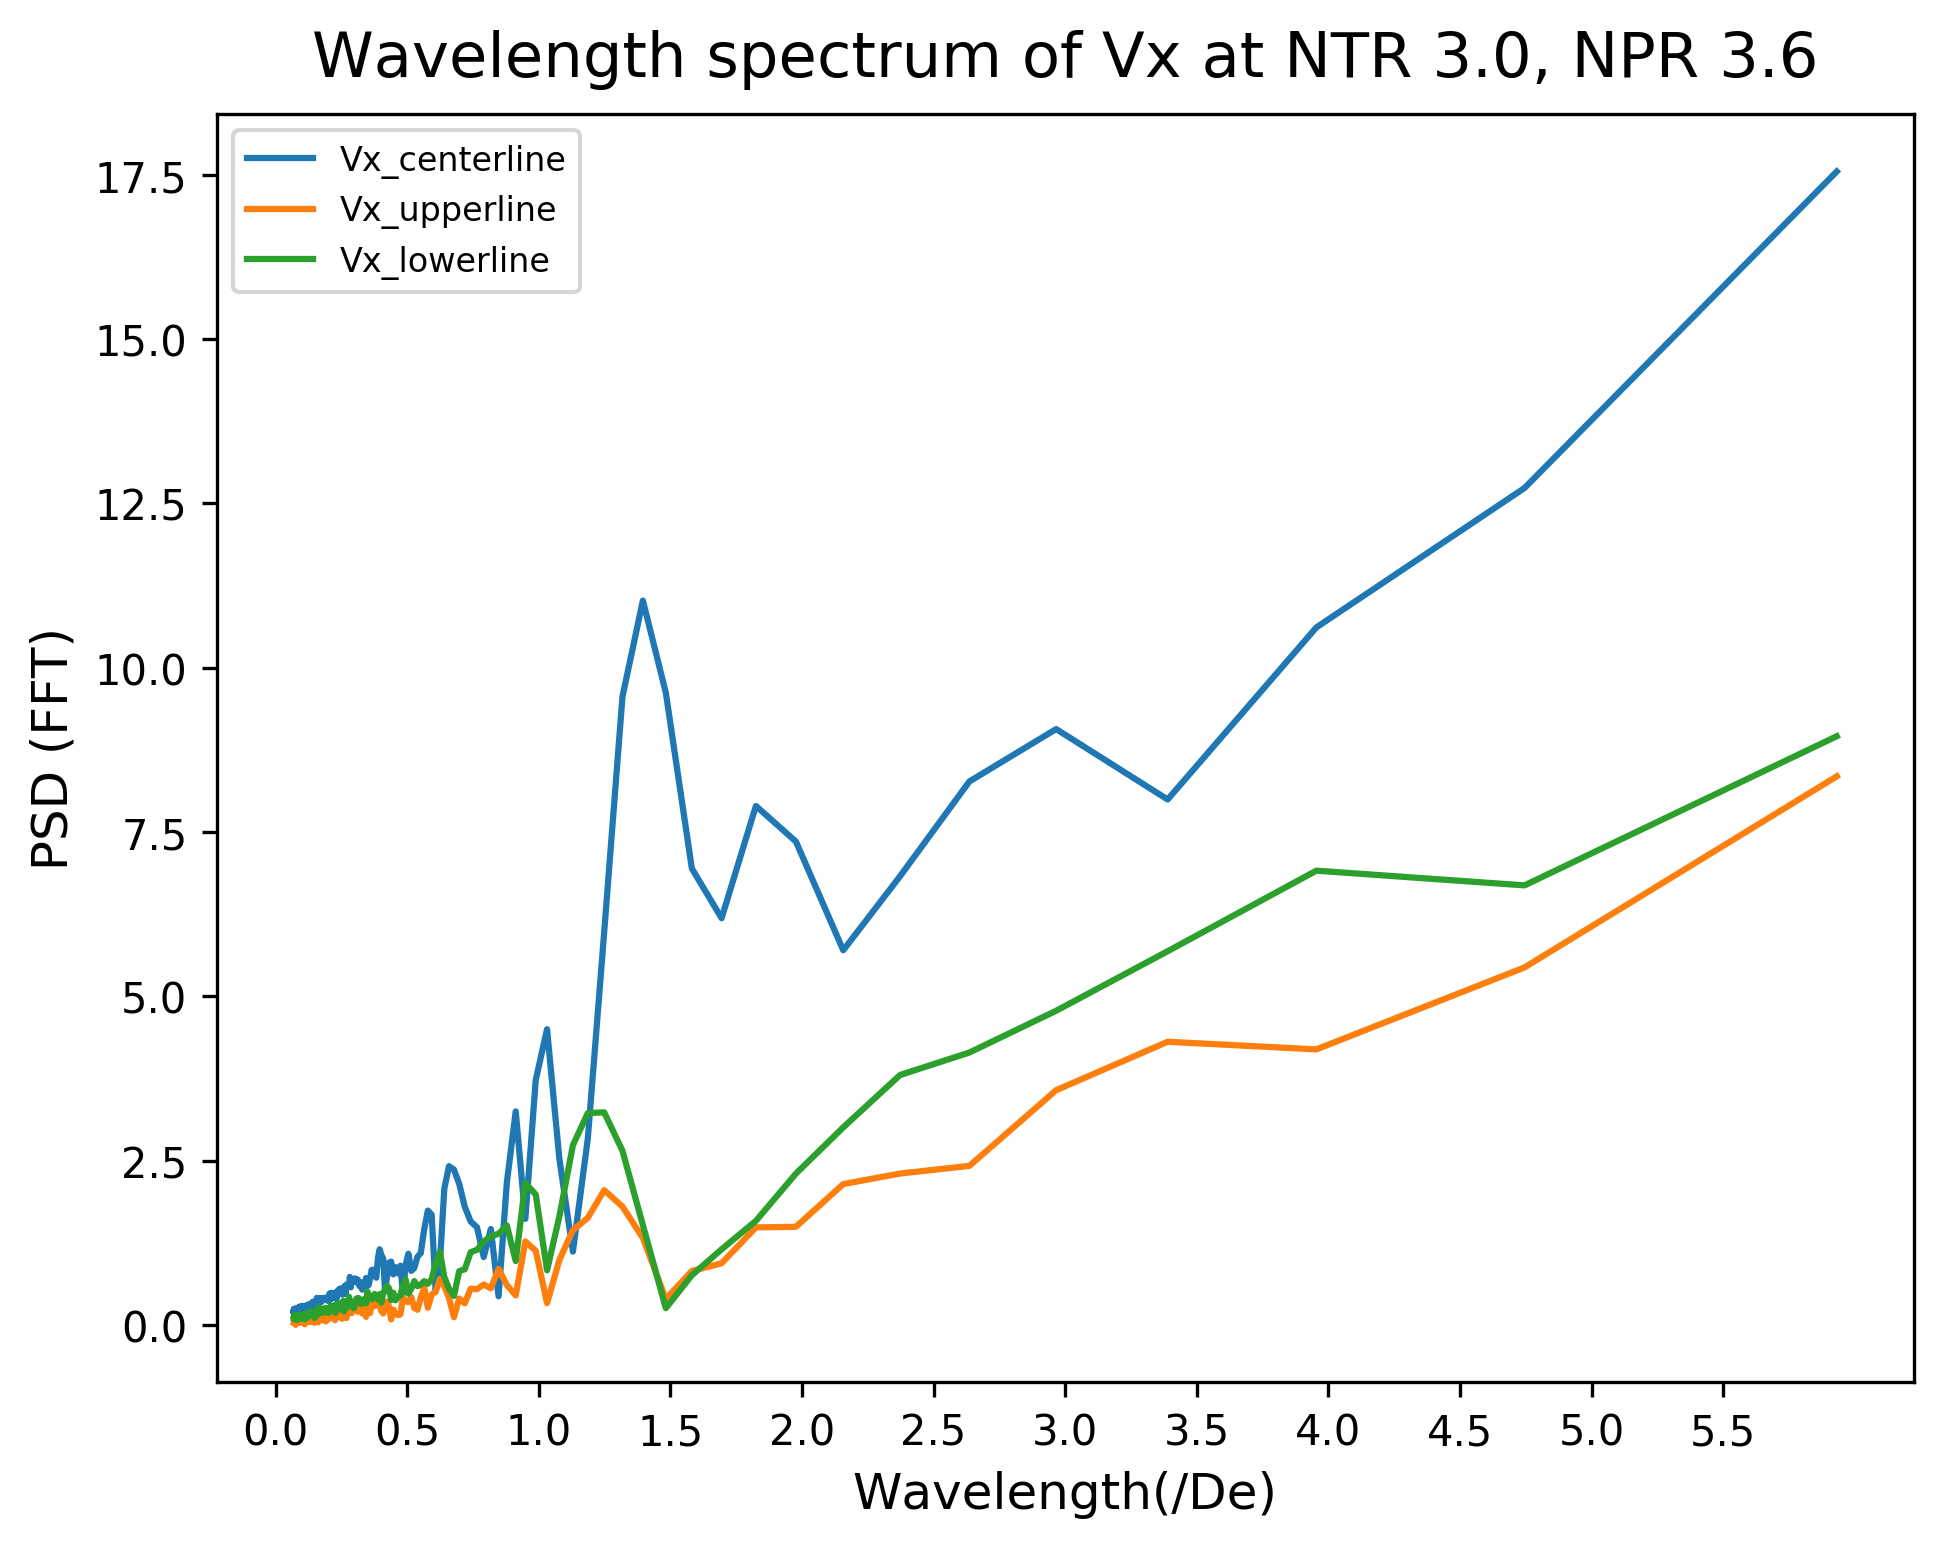
\includegraphics[width=3in]{images/Fft_Vx_NTR3p0_NPR3p6c.png}
	\caption{NTR:3p0 NPR:3p6 with chevrons}
	\label{fig:setup1}
\end{subfigure}%
\caption{wavelength spectrum using FFT for centreline $V_x$ with  chevrons }
\label{fig:fftplotsc}
\end{figure}

Another interesting observation (fig \ref{fig:lineplotsTKE}) is considerable increase in TKE fluctuations on centreline because of chevrons although TKE at lips of jet is not affected much. Reduction in screech tone with chevrons, widely observed, can still be explained with possible increase in difference between frequencies of acoustic waves exciting thin shear layer and flow structure-shock interaction. But reduction in BBSN amplitude as reported in Heeb et.al.\cite{heeb} is counterintuitive with what is being observed here and shows that influence of chevrons on BBSN needs more attention. 

\begin{figure}[H]
\begin{subfigure}{.5\textwidth}
	\centering
	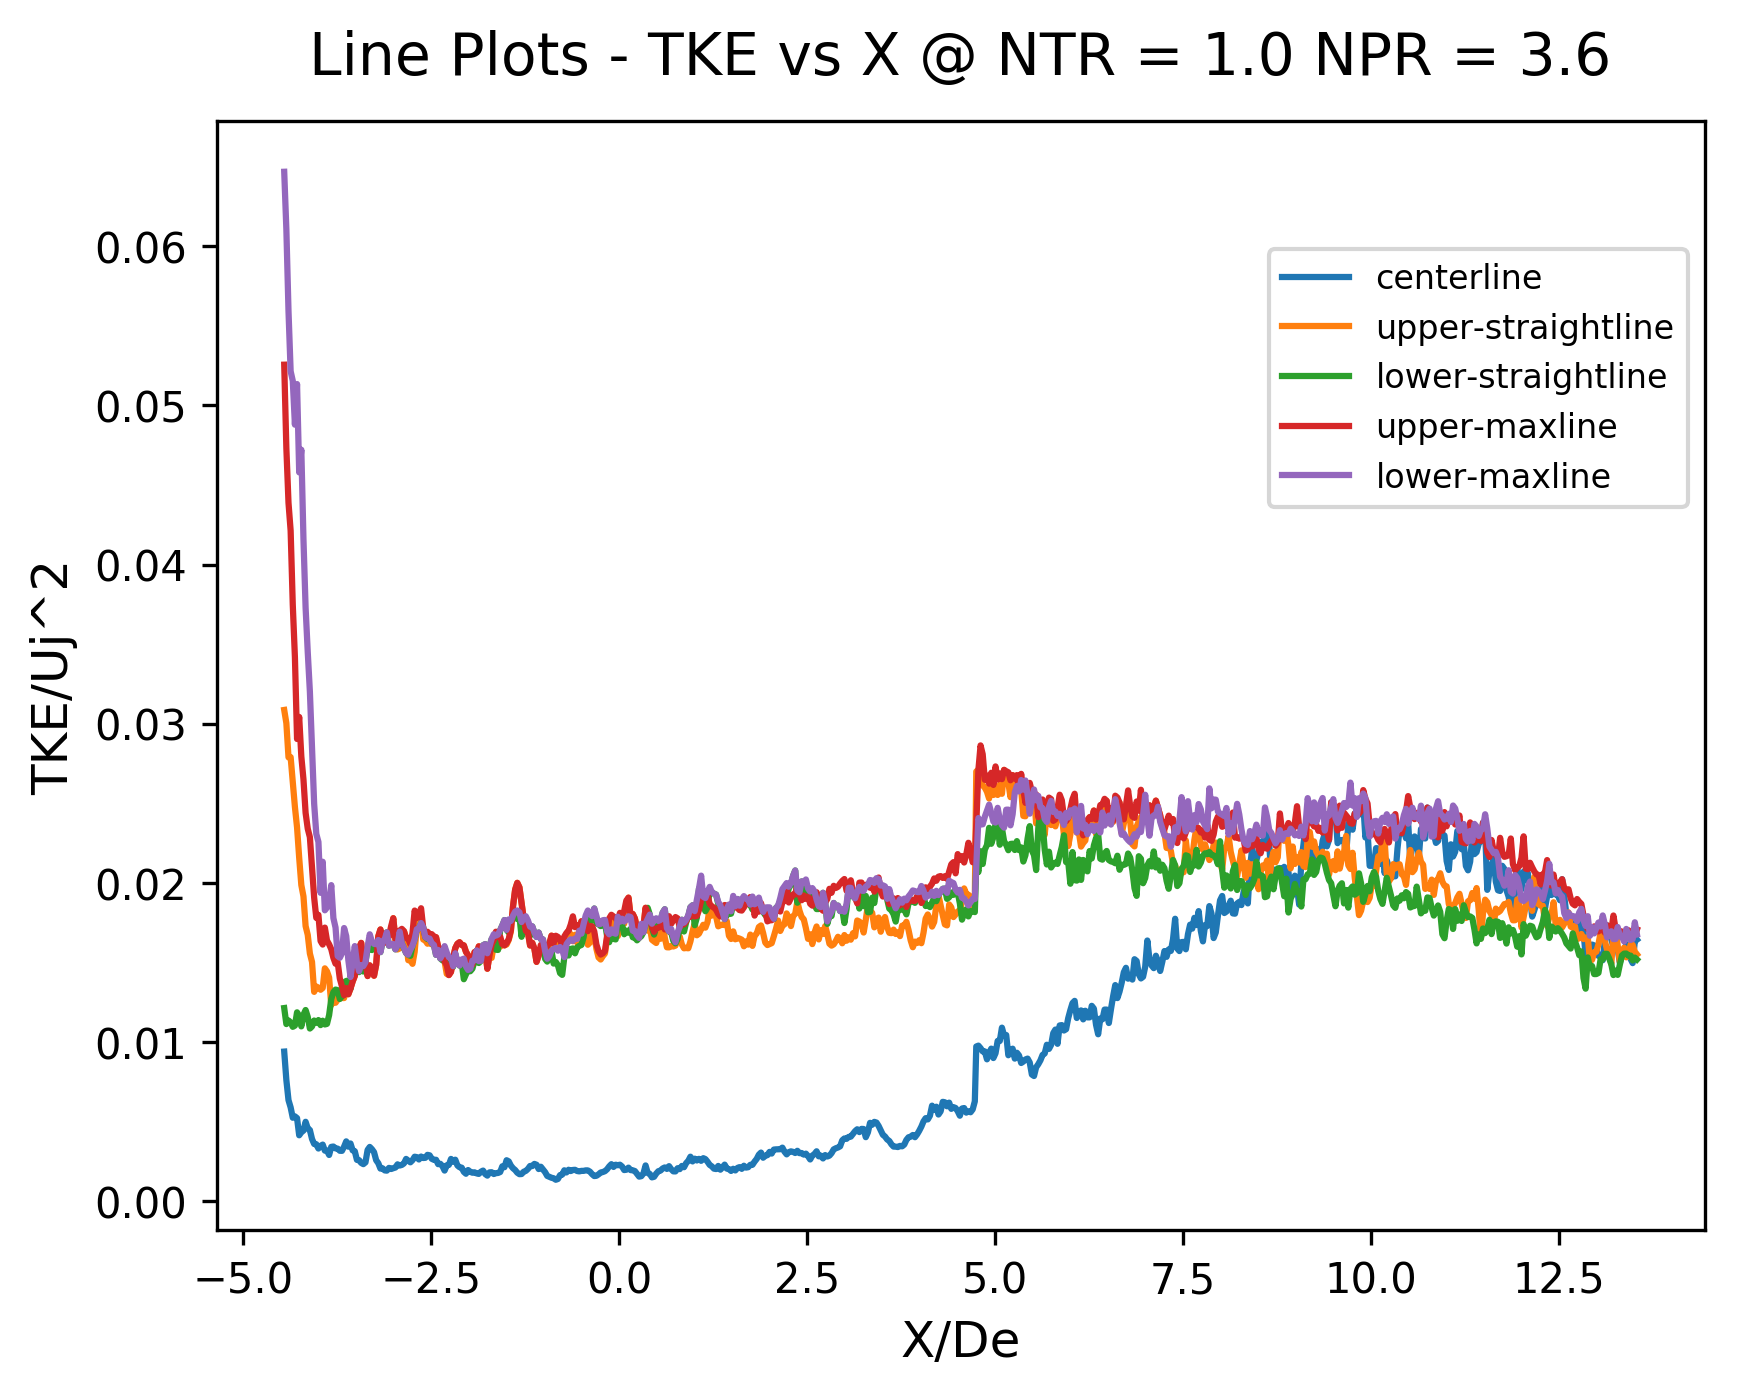
\includegraphics[width=2.5in]{images/LinePlots_TKE_NTR1p0_NPR3p6.png}
	\caption{NTR:1p0 NPR:3p6 without chevrons }
	\label{fig:setup1}
\end{subfigure}%
\begin{subfigure}{.5\textwidth}
	\centering
	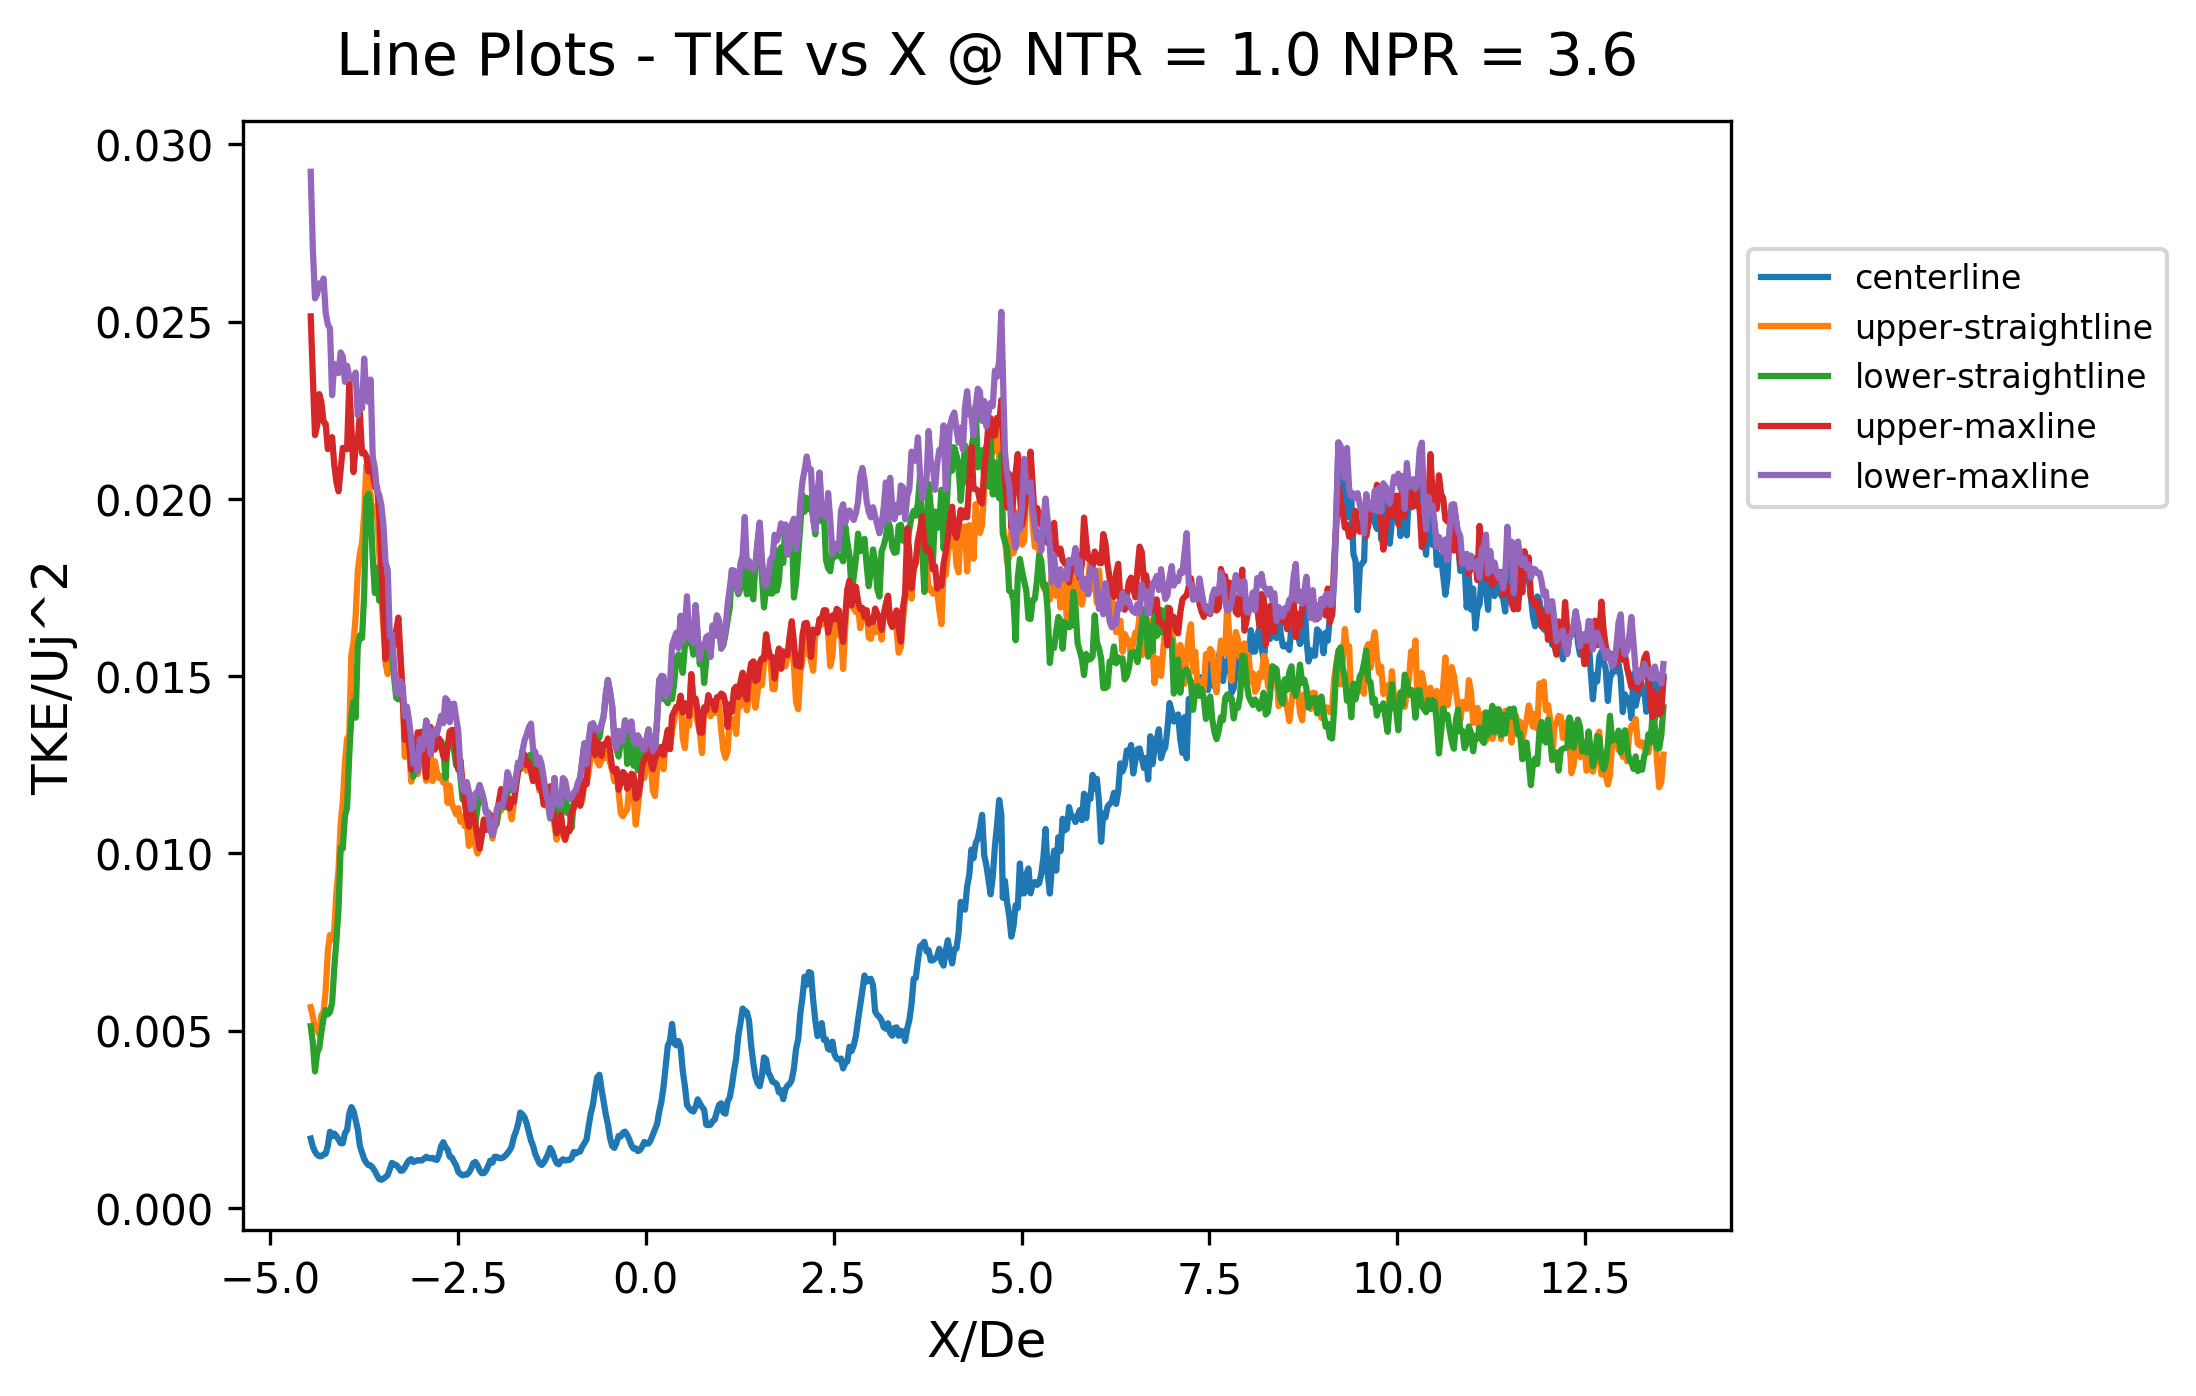
\includegraphics[width=3in]{images/LinePlots_TKE_NTR1p0_NPR3p6c.png}
	\caption{NTR:1p0 NPR:3p6 with chevrons}
	\label{fig:setup2}
\end{subfigure}
\begin{subfigure}{.5\textwidth}
	\centering
	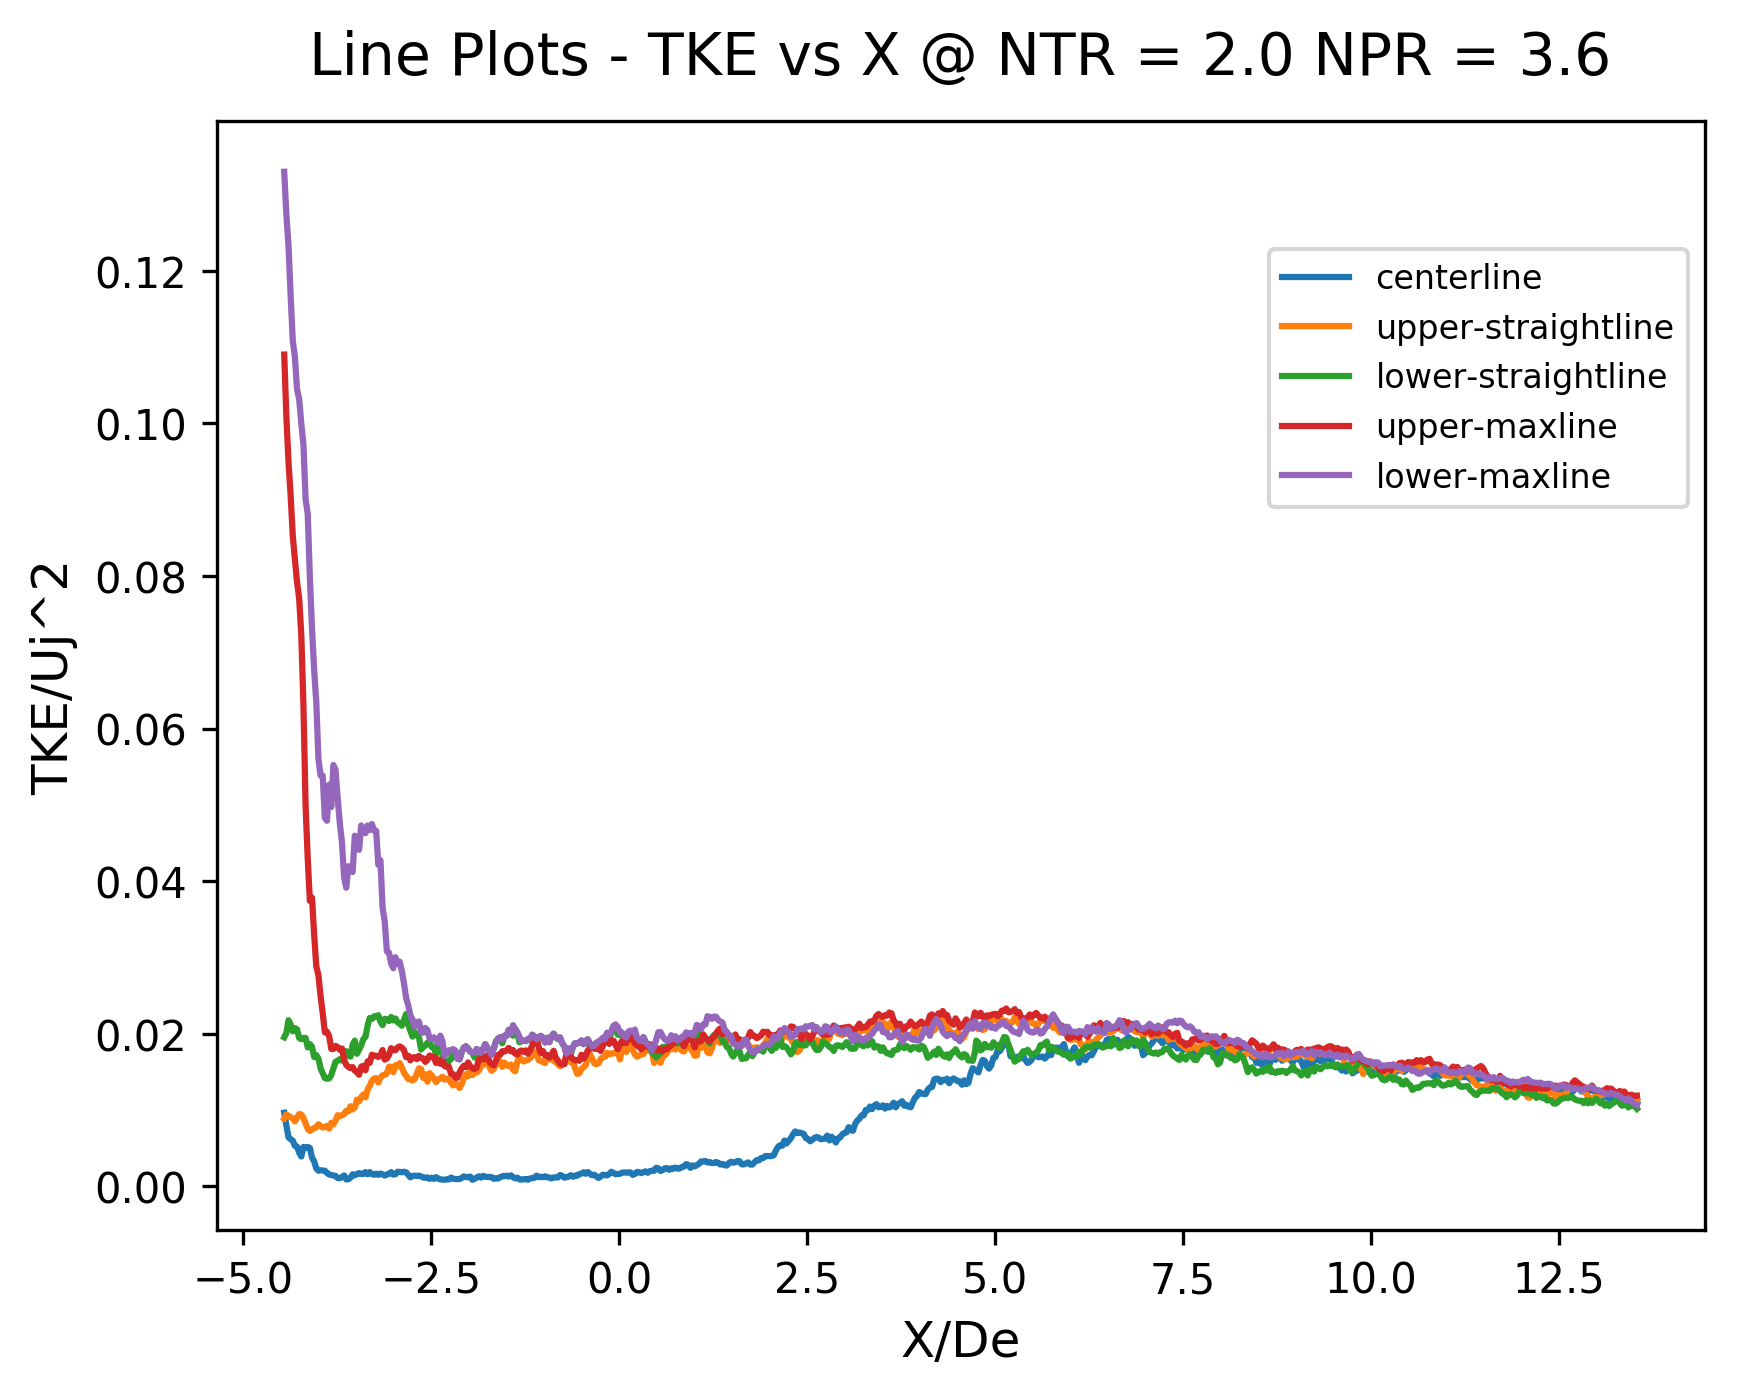
\includegraphics[width=2.5in]{images/LinePlots_TKE_NTR2p0_NPR3p6.png}
	\caption{NTR:2p0 NPR:3p6 without chevrons}
	\label{fig:setup1}
\end{subfigure}%
\begin{subfigure}{.5\textwidth}
	\centering
	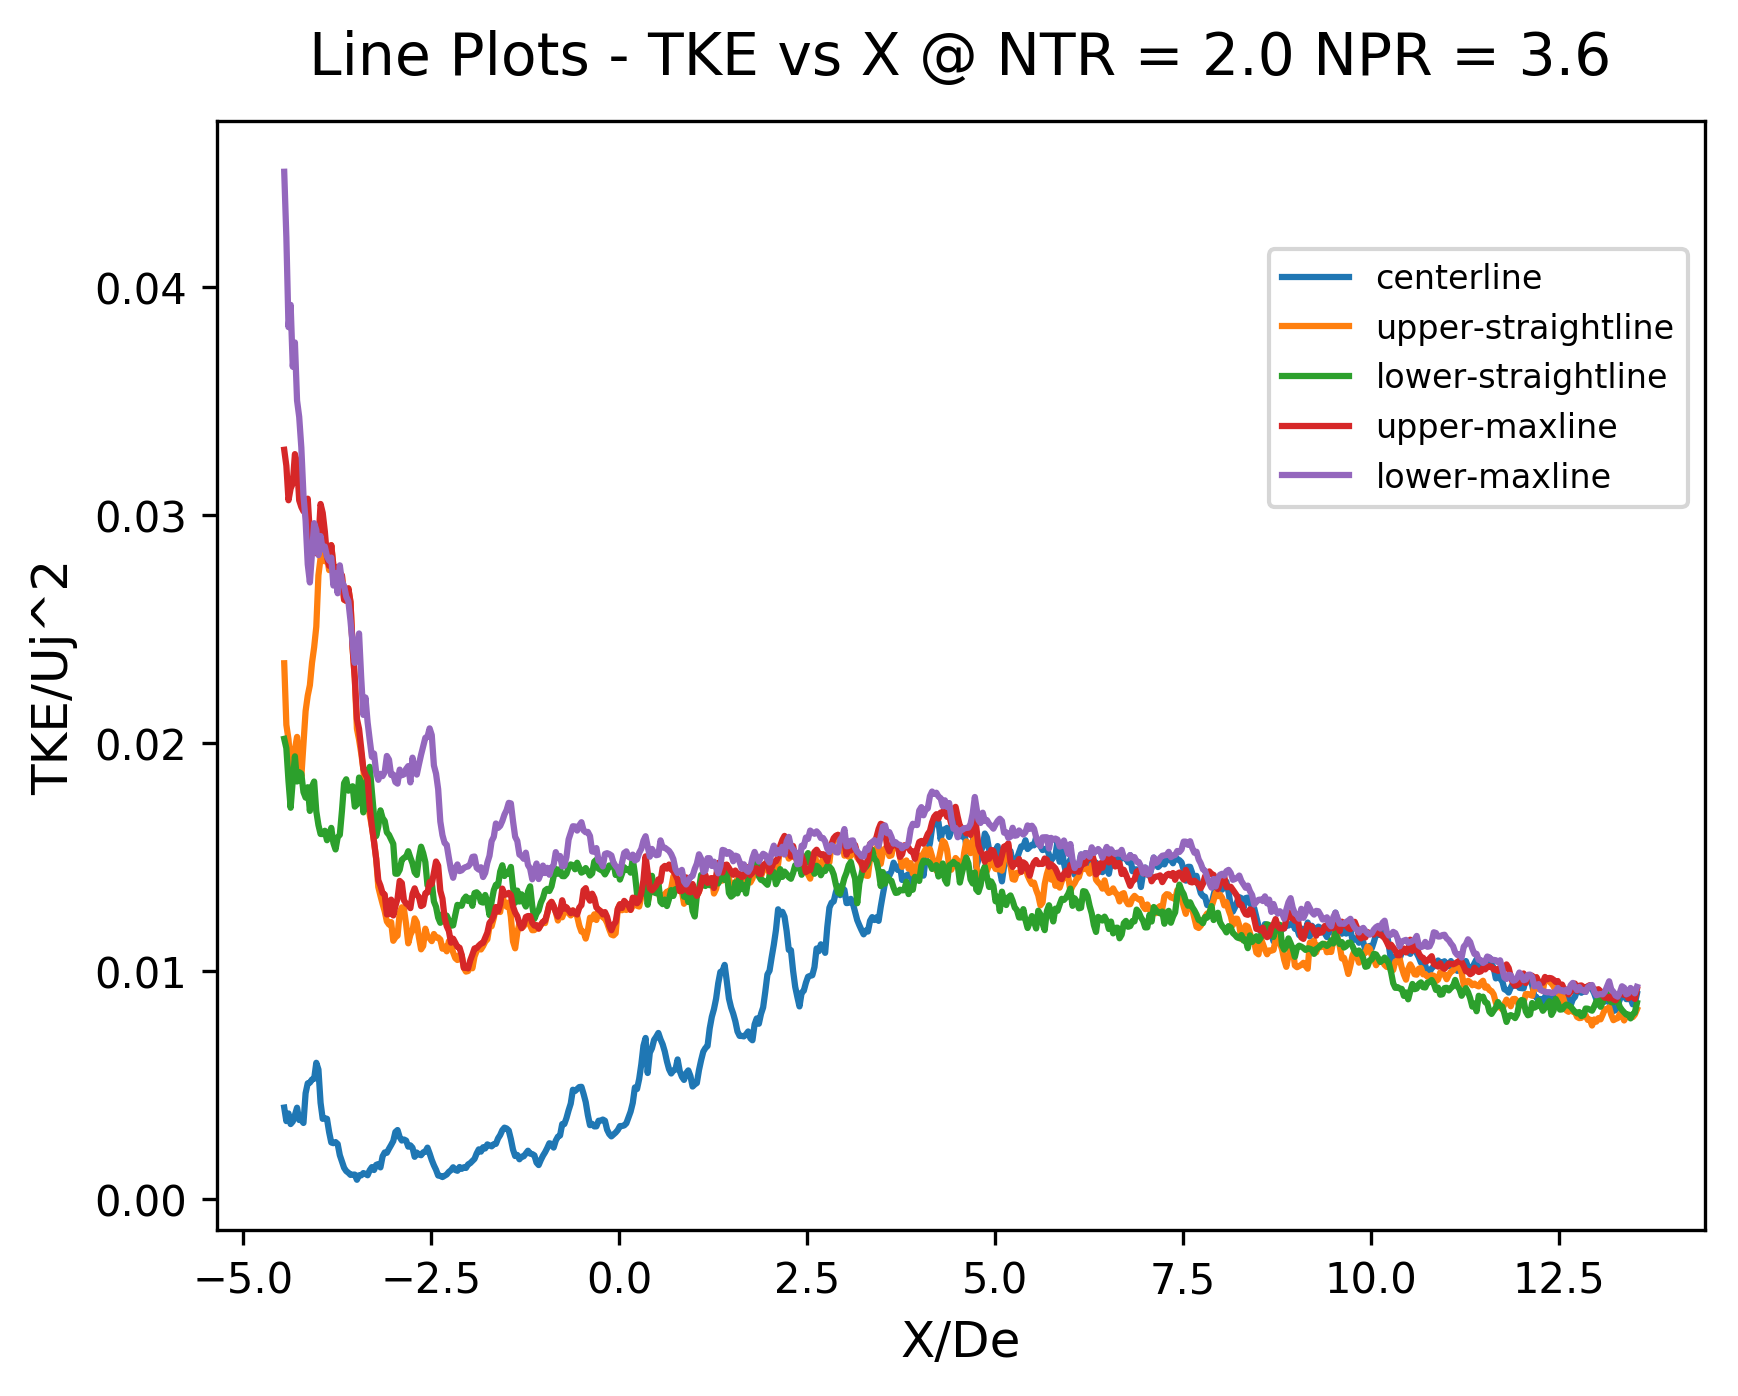
\includegraphics[width=2.5in]{images/LinePlots_TKE_NTR2p0_NPR3p6c.png}
	\caption{NTR:2p0 NPR:3p6 with chevrons}
	\label{fig:setup2}
\end{subfigure}
\begin{subfigure}{.5\textwidth}
	\centering
	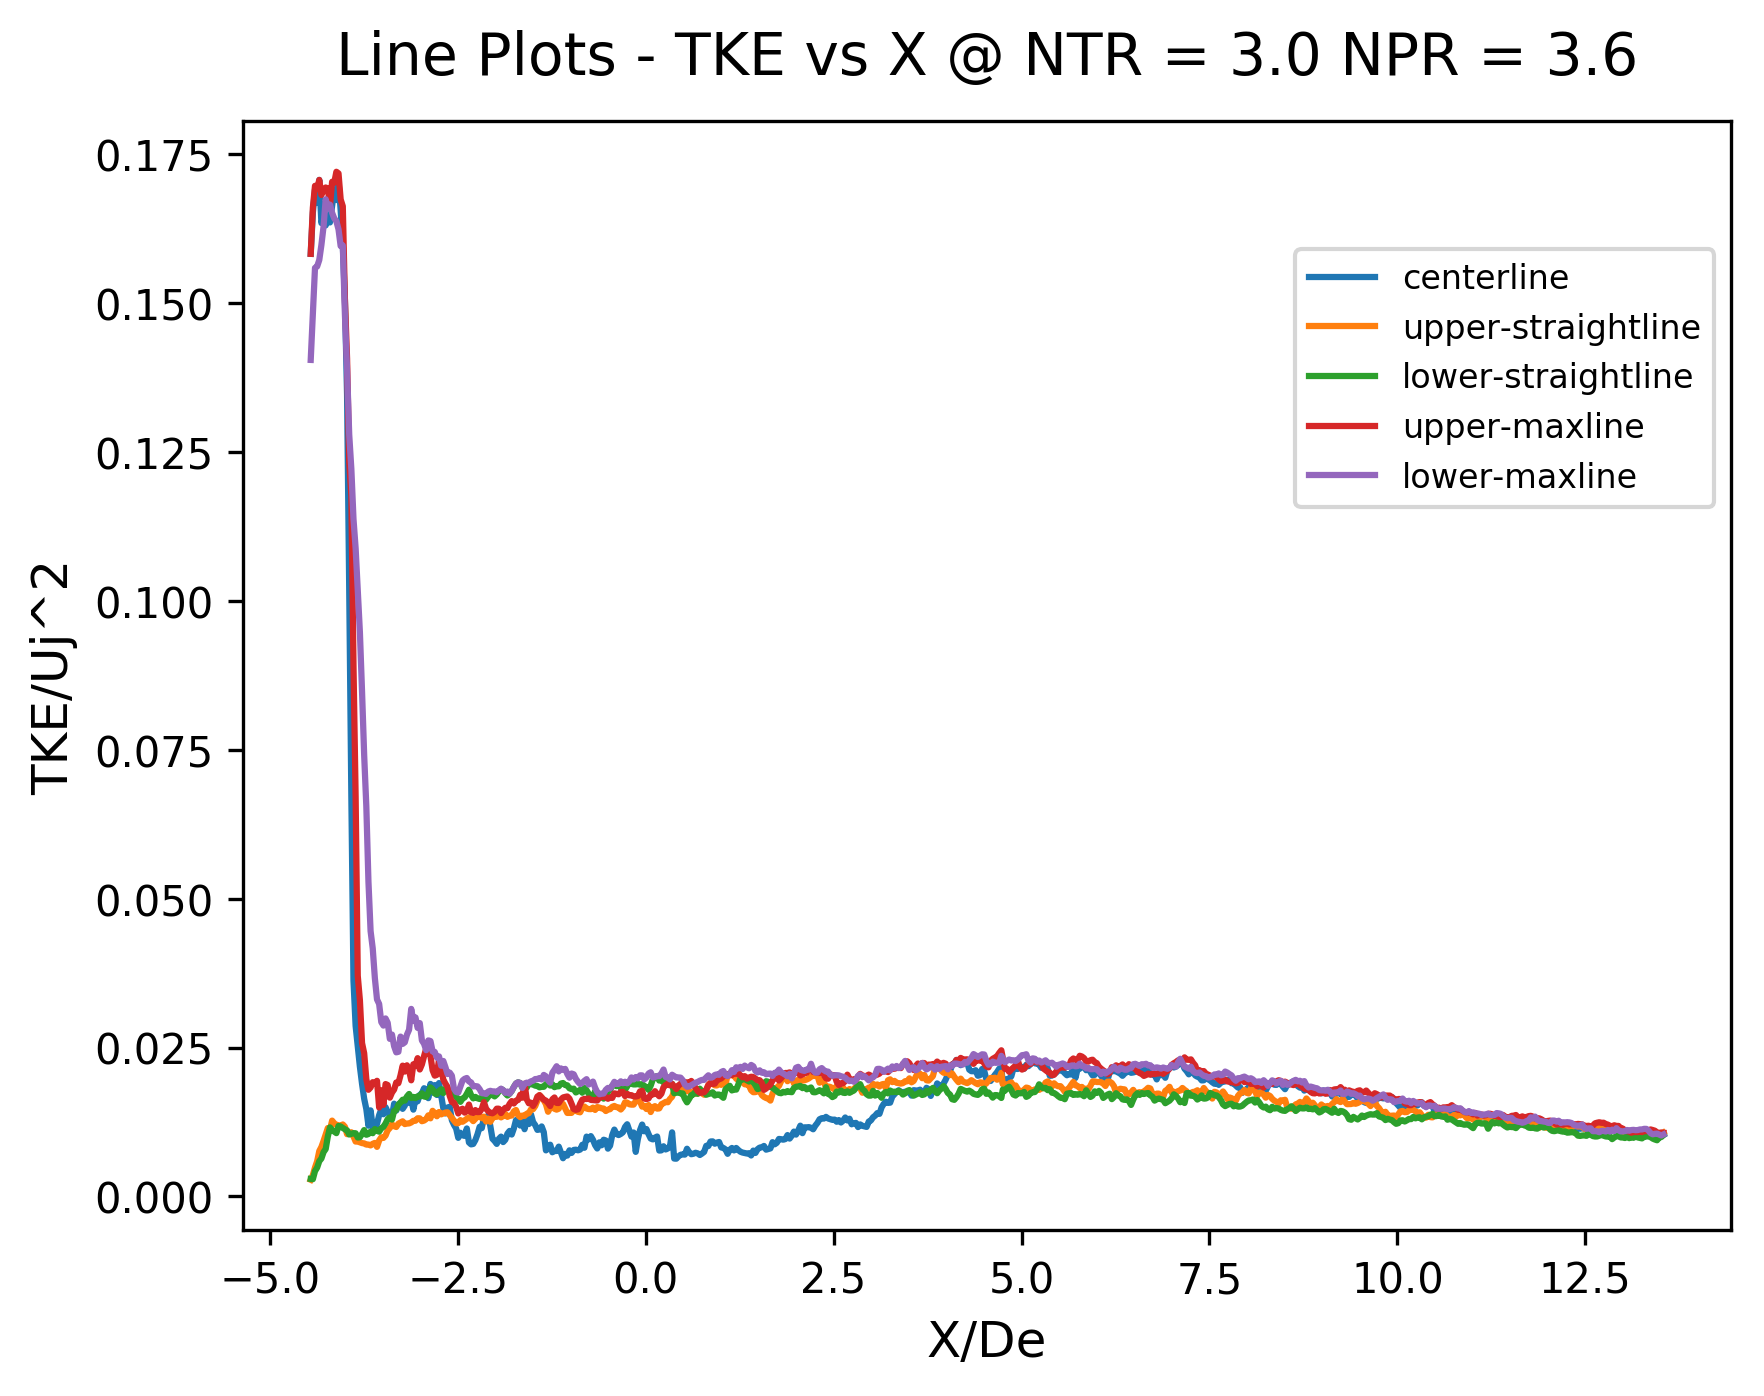
\includegraphics[width=2.5in]{images/LinePlots_TKE_NTR3p0_NPR3p6.png}
	\caption{NTR:3p0 NPR:3p6 without chevrons}
	\label{fig:setup1}
\end{subfigure}%
\begin{subfigure}{.5\textwidth}
	\centering
	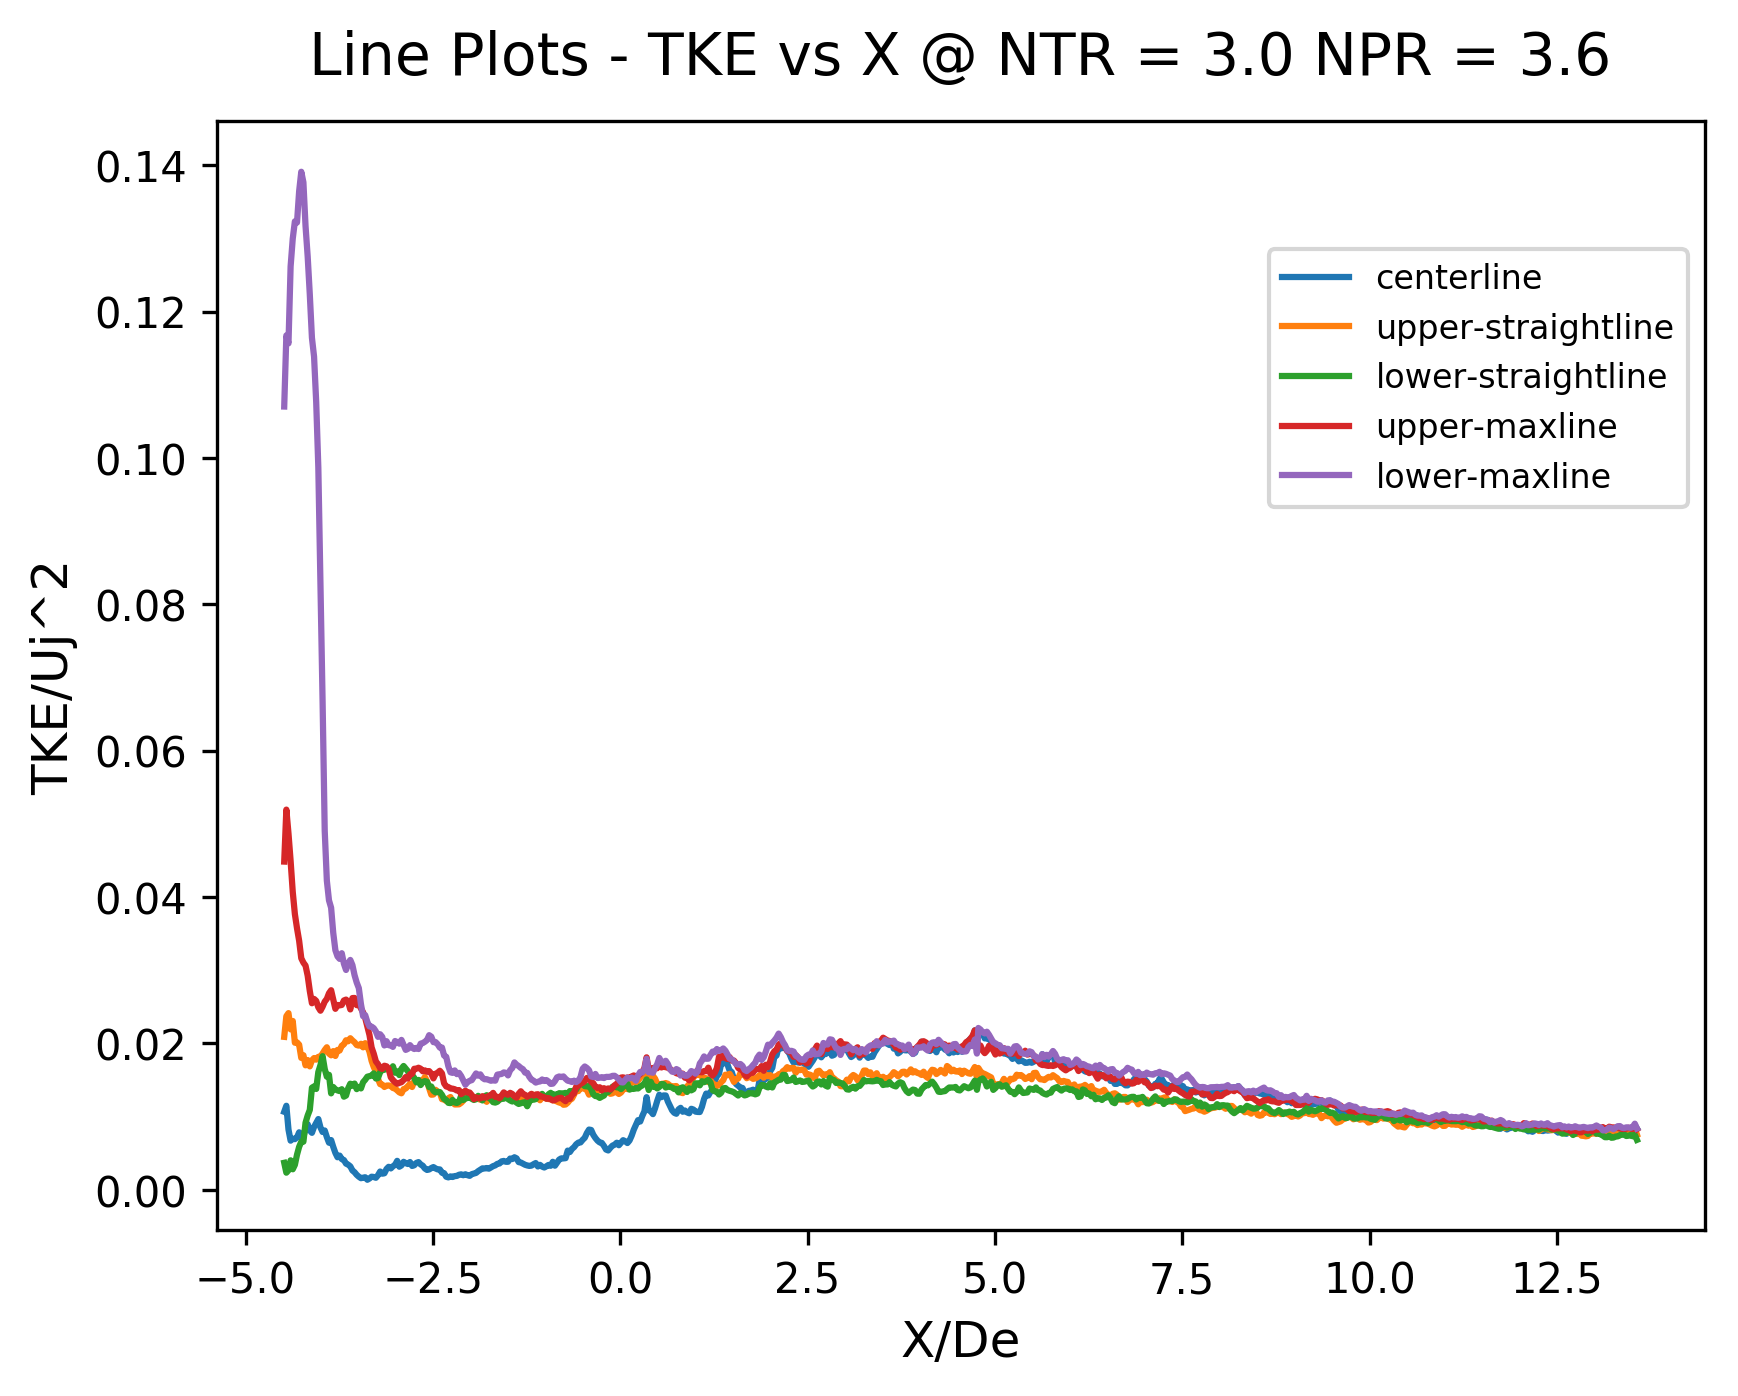
\includegraphics[width=2.5in]{images/LinePlots_TKE_NTR3p0_NPR3p6c.png}
	\caption{NTR:3p0 NPR:3p6 with chevrons}
	\label{fig:setup2}
\end{subfigure}
\caption{centreline plots for TKE with and without chevrons }
\label{fig:lineplotsTKE}
\end{figure}

\section{Summary}

Various visualization techniques, including FFT and spectogram, have been used to gather as much information as possible from velocity, TKE of steady PIV data. Shock cell lengths observed are compared with analytical values. Effect of pressure, temperature, chevron including conflicts and agreements with published data is discussed. 

%\end{document}